\documentclass[mathserif]{beamer}
\usepackage{beamerthemeshadow}
\usepackage{beamerthemesplit}
%\usetheme{shadow}
\usecolortheme{default}
\setbeamertemplate{footline}[frame number]
\useinnertheme[shadow=true]{rounded}
%\setbeamertemplate{footline}{\insertframenumber/\inserttotalframenumber}
%\useoutertheme{infolines}
%\setbeamertemplate{headline}{} % removes the headline that infolines inserts


%\usetheme{boxes}
%\usepackage{amsmass}
%\usepackage{amssymb,amsfonts,url}

\usepackage{algorithm}
\usepackage{algorithmic}

\usepackage{graphicx}
\graphicspath{{Problems/}}

\usepackage{caption}
\captionsetup[figure]{labelformat=simple}
\captionsetup[table]{labelformat=simple}


\usepackage{tikz}
\usetikzlibrary{shadows}
\usetikzlibrary{positioning}
\usepackage{verbatim}
\usepackage{pgfplots}
\usepackage{verbatim}
\usetikzlibrary{arrows,shapes}

\definecolor{darkblue}{rgb}{0.2,0.2,0.6}
\definecolor{darkred}{rgb}{0.6,0.1,0.1}
\definecolor{darkgreen}{rgb}{0.2,0.6,0.2}

\usetikzlibrary{shadings,shadows,shapes.arrows}

\usetikzlibrary{calc} 
\makeatletter 
\@namedef{color@3}{blue!20}
\@namedef{color@1}{green!70}   
%\@namedef{color@3}{yellow!50} 
\@namedef{color@2}{orange!90}  
%\@namedef{color@5}{magenta!70} 
%\@namedef{color@6}{yellow!70}    

\newcommand{\graphitemize}[2]{%
\begin{tikzpicture}[every node/.style={align=center}, scale=0.78]  
 \draw[fill=green!5, fill opacity=0.1, green, inner sep=0.05cm, outer sep=0.05cm] (5,0) arc(0:360:5);
 % \draw[fill=white, fill opacity=0.1, white, inner sep=0.05cm, outer sep=0.05cm] (4,0) arc(0:360:4);
%  \shade[ball color=gray!10!] (0,0) coordinate(Hp) circle (.9);
  \node[shape=circle,  minimum size=1.1cm,fill=red!60,font=\Large,outer sep =.15cm,inner sep=.2cm,drop  shadow={ashadow, color=red!60!black}](ce){#1};  
   % \shade[ball color=blue!20!] (0,0) coordinate($Algorithm$) circle (1.5cm);

\foreach \gritem [count=\xi] in {#2}  {\global\let\maxgritem\xi}  
\foreach \gritem [count=\xi] in {#2}
{% 
\pgfmathtruncatemacro{\angle}{90+360/\maxgritem*\xi}
\edef\col{\@nameuse{color@\xi}}
\node[shape=circle,
     ultra thick,
     draw=white,
     fill opacity=1,
     drop  shadow={ashadow, color=blue!60},
     fill=\col,outer sep=0.25cm,        
     minimum size=2cm] (satellite-\xi) at (\angle:5cm) {\gritem };
     \draw[line width=0.25cm,-latex, \col] (ce) -- (satellite-\xi);
     }%
% \draw[violet, fill=violet!10] (4,0) arc(0:360:4);
\end{tikzpicture}  
}%



\newcommand*{\tikzarrow}[2]{%
  \tikz[
    baseline=(A.base),             % Set baseline to the baseline of node content
    font=\footnotesize\sffamily    % Set fontsize of the node content
  ]
  \node[
    single arrow,                  % Shape of the node
    single arrow head extend=2pt,  % Actual width of arrow head
    draw,                          % Draw the node shape
    inner sep=2pt,                 % Separation between node content and node shape
    top color=white,               % Shading color on top of node
    bottom color=#1,               % Shading color on bottom of node
    drop shadow                    % Draw a shadow
  ] (A) {#2};%
}


\def\arrow{
  (10.05:1.1) -- (6.05:1) arc (6.05:120:1) [rounded corners=0.5] --
  (120:0.9) [rounded corners=1] -- (130:1.1) [rounded corners=0.5] --
  (120:1.3) [sharp corners] -- (120:1.2) arc (120:5.25:1.2)
  [rounded corners=1] -- (10.05:1.1) -- (6.05:1) -- cycle
}

\tikzset{
  ashadow/.style={opacity=.25, shadow xshift=0.07, shadow yshift=-0.07},
}

\def\arrows[#1]{         
  \begin{scope}[scale=#1]
    \draw[color=darkred, drop  shadow={ashadow, color=red!60!black}] \arrow;

    \draw[color=darkgreen, bottom color=green!90!black, top color=green!60,   drop shadow={ashadow, color=green!60!black}] [rotate=120] \arrow;

    \draw[color=darkblue, right color=blue, left color=blue!60,   drop shadow={ashadow, color=blue!60!black}] [rotate=240] \arrow;

    % to hide the green shadow
    \draw[color=darkred, left color=red, right color=red!60] \arrow;
  \end{scope}
}


\tikzstyle{vertex}=[circle,fill=black!25,draw,minimum size=20pt,inner sep=0pt]
\tikzstyle{smallvertex}=[circle,fill=black!25,draw,minimum size=10pt,inner sep=0pt]
\tikzstyle{selected vertex} = [vertex, draw,fill=red!24]
\tikzstyle{blue smallvertex} = [smallvertex, draw,fill=blue]
\tikzstyle{red smallvertex} = [smallvertex, draw,fill=red]
\tikzstyle{edge} = [draw,thick,->]
\tikzstyle{undirectededge} = [draw,thick]
\tikzstyle{weight} = [font=\small]
\tikzstyle{selected edge} = [draw,line width=5pt,-,red!50]
\tikzstyle{ignored edge} = [draw,line width=5pt,-,black!20]
\tikzstyle{squarednode}=[draw, fill=blue!20, thick, minimum size=5mm]
\tikzstyle{roundnode}=[circle, draw, fill=blue!20, thick, minimum size=5mm]



%\usepackage{CJK}
%\usepackage{pinyin}

%    \begin{figure}
%        \centering
%        \includegraphics[width=0.8\textwidth]{newGeneRep.eps}
%    \end{figure}

% \begin{figure}%
%   \begin{center}%
%     \begin{minipage}{0.70\textwidth}%
%      \includegraphics[width=1.0\textwidth]{comp25000.eps}%
%     \end{minipage}%
%     \begin{minipage}{0.30\textwidth}
%      \includegraphics[width=1.0\textwidth]{comparelabel.eps}%
%     \end{minipage}%
%   \end{center}
% \end{figure}

% \begin{table}
%   {\begin{tabular}{l|rrr}\hline
%       & \multicolumn{3}{c}{Actual number of DCJ operations}\\
%       \# genes &\# genes $\times 1$&\# genes $\times 2$&\# genes  $\times 3$ \\
% \hline
%      (a)~25,000 & 0.5\% ~~&  0.9\% ~~& 1.7\%~~\\
%       (b)~10,000 & 0.8\%~~ &  1.4\% ~~& 2.7\%~~\\
%      (c)~ 1,000 & 2.7\%~~ & 4.7\%~~ & 14.7\%~~\\ \hline
%     \end{tabular}} {}%
% \end{table}

% \begin{eqnarray}
% T(n) &=&  \sum_{i=1}^n C_i \\
%      &=&  \# PUSH + \#POP \\
%      &<& 2\times \#PUSH \\
%      &<& 2n \\
% \end{eqnarray}


\title{CS711008Z Algorithm Design and Analysis }
\subtitle{ Lecture 5. Basic algorithm design technique: {\sc Divide and Conquer} 
%	\footnote{The slides are prepared based on Chapter 2 and 28 of Introduction to algorithms, Chapter 5 of Algorithm design. Some slides are excerpted from the slides by Kevin Wayne with permission.} 
}
\author{Dongbo Bu \\
\ \ \ \ \ \ \ \ \ \ \ \ \ \ \ \ \ \ \ \ \ \ \ \ \ \ \ \ \ \ \ \ \ \ \ \ \ \ \ \ \ \ \ \ \ \ \ \ \ \ \ \ \ \ \ \ \ \ \ \ \ \ \ \ \ \ \ \ \ \ \ \ \ \ \ \ \ \ \ \ \ \ \ \ \ \ \ \ \ \ \ \ \ \ \ \ \ \ \ \  \\
{\small Institute of Computing Technology \\ Chinese Academy of Sciences, Beijing, China}}
\date{}


\begin{document}
%\begin{CJK}{UTF8}{cyberbit}

\frame{\titlepage}


\frame{
\frametitle{Outline}
\begin{itemize}
 \item The basic idea of {\sc Divide and Conquer} technique; 
 \item The first example: {\sc MergeSort} \\
	\begin{itemize}
		\item Correctness proof by using \textcolor{red}{{\bf loop invariant}}
		technique;
		\item Time complexity analysis of recursive algorithm.
	\end{itemize}
 \item Other examples:  {\sc CountingInversion}, {\sc ClosestPair}, {\sc Multiplication}, {\sc FFT}; 
 \item Combining with randomization: {\sc QuickSort}, {\sc QuickSelect}, {\sc BFPRT} and {\sc FloydRivest} algorithm for {\sc Selection} problem; 
 \item Remarks: 
\begin{enumerate}
 \item 
{\sc Divide and Conquer}  could serve to reduce the running time though \textcolor{red}{\bf the 
brute-force algorithm is already polynomial-time}, say the $O(n^2)$ brute-force algorithm versus $O(n \log n )$ divide and conquer algorithm for the {\sc ClosestPair} problem.
\item 
This technique is especially powerful when \textcolor{red}{\bf combined with randomization technique. } 
\end{enumerate}
\end{itemize}
}

\frame{
\frametitle{The general {\sc {\sc Divide and Conquer}} paradigm }
%\begin{figure}
% \includegraphics[width=1.5in] {L5-dc.eps}
%\end{figure}
\begin{itemize}
    \item 
Basic idea: Many problems are recursive in structure, i.e., to solve a given problem, they call themselves several times to deal with closely related \textcolor{blue}{\bf sub-problems}. These sub-problems have the same form to the original problem but a smaller size.\\
	\item 
Three steps of the {\sc {\sc Divide and Conquer}} paradigm: 

\begin{enumerate}
 \item \textcolor{blue}{\bf Divide}  a problem into a number of \textcolor{blue}{\bf independent sub-problems}; \\
%How to divide? \textcolor{red}{at middle-point; divide into two parts with odd- andeven- indices; enumerate all cases of dividing point; randomly choose one, etc.}
 \item \textcolor{blue}{\bf Conquer} the subproblems by solving them recursively; 
 \item \textcolor{blue}{\bf Combine} the solutions to the subproblems into the solution to the original problem. 
 %  \\Sometimes clever ideas are needed to combine. 	
\end{enumerate}
\end{itemize}

} 

\frame{
	\frametitle{Peng's saying}
	
	\begin{figure}
		\includegraphics[width=4in]{L5-Divide-and-conqueror-Peng.png}
	\end{figure}
}

\frame{
	\frametitle{{\sc Divide and Conquer} technique}
	\begin{itemize}
		\item To see whether the {\sc Divide and Conquer} technique applies on a given problem, we need to examine both \textcolor{red}{\bf  input} and \textcolor{red}{\bf output} of the problem description. 
		\begin{itemize}
			\item Examine the \textcolor{red}{\bf  input}  part to determine how to decompose the problem into subproblems of same structure but smaller size: It is relatively easy to decompose a problem into subproblems  if the input part is related to the following data structures:
			\begin{itemize}
				\item An \textcolor{red}{\bf array} with $n$ elements; 
				\item A \textcolor{red}{\bf matrix}; 
				\item A \textcolor{red}{\bf set} of $n$ elements;
				\item A \textcolor{red}{\bf tree}; 
				\item A \textcolor{red}{\bf directed acyclic graph};
				\item A \textcolor{red}{\bf general graph}.
			\end{itemize}
			\item Examine the \textcolor{red}{\bf output} part to determine how to construct the solution to the original problem using the solutions to its subproblems. 
		\end{itemize}

	\end{itemize}
}


\frame{
\begin{block}{}
{\sc Sort} problem: to sort an \textcolor{red}{\bf array} of $n$ integers
\end{block}
}

\frame{
\frametitle{}
{\sc Sort} problem
\begin{block}{}
 {\bf INPUT: } An array of $n$ integers, denoted as $A[0..n-1]$; \\
 {\bf OUTPUT: } The elements of $A$ in increasing order.
\end{block}

	\begin{figure}
		\includegraphics[width=2.5in]{L5-sort-example3.png}
	\end{figure}

\begin{itemize}
	\item An array can be divided into smaller ones based on \textcolor{red}{\bf indices} or \textcolor{red}{\bf values} of elements.  
\end{itemize}

}


\frame{
\frametitle{Divide strategy 1 based on indices of elements} 

\begin{itemize}
 \item \textcolor{red}{\bf Divide array $A[0..n-1]$ into a $n-1$-length array $A[0..n-2]$ and a single element}:  $A[0..n-2]$ has the same form to $A[0..n-1]$ but smaller size; thus, sorting $A[0..n-2]$ constructs a subproblem of the original problem. The {\sc Divide and Conquer} strategy might apply if we can sort $A[0..n-1]$ using the sorted $A[0..n-2]$.  

\begin{figure}
    
\begin{tikzpicture}[scale=1.0, auto,swap]
  
    \foreach \i/\name in { 0/A_0,1/A_1,2/\hdots,3/A_{n-2},4/A_{n-1} } {
         \draw[  black, thick ] (\i,0) rectangle (\i+1, 0.618);
         \node at (\i+0.5, 0.618/2) {$\name$};
    }
 
   \draw[very thick, blue] (4,-0.2) -- (4, 0.618+0.2);
   \draw[ -latex, blue, line width=3pt ] (4, -0.5) -- (4, -1.2 ); 


     \foreach \i/\name in { 0/A_0,1/A_1,2/\hdots,  3/A_{n-2}} {
         \draw[  black, thick ] (\i-0.3,0-2) rectangle (\i+1-0.3, 0.618-2);
         \node at (\i+0.5-0.3, 0.618/2-2) {$\name$};
     }
 
      \foreach \i/\name in { 4/A_{n-1} } {
         \draw[  black, thick ] (\i+0.3,0-2) rectangle (\i+1+0.3, 0.618-2);
         \node at (\i+0.5+0.3, 0.618/2-2) {$\name$};
    }
\end{tikzpicture}
\end{figure}

\end{itemize}
}





\frame{
\frametitle{Sort $A[0..n-1]$ using the sorted $A[0..n-2]$} 

%\begin{figure}
% \includegraphics[width=1.3in] {L5-incremental.eps}
%\end{figure}

\begin{itemize}
 \item 
Basic idea: To sort $A[0..n-1]$, it suffices to put $A[n-1]$ in its correct position among the sorted $A[0..n-2]$, which can be achieved through comparing $A[n-1]$  with the elements in $A[0..n-2]$. 
\end{itemize} 

%\begin{figure}
%   
%\begin{tikzpicture}[scale=0.9, auto,swap]
% 
%\def\dy{-2.5}; 
%  \foreach \i/\name in { 0/A_0,1/A_1 } {
%         \draw[  green, thick ] (\i,0 + \dy) rectangle (\i+1, 0.618 + \dy);
%         \node at (\i+0.5, 0.618/2 + \dy) {$\name$};
% }
%   \foreach \i/\name in { 0/A_0 } {
%         \draw[  red, thick ] (\i,0 + \dy) rectangle (\i+1, 0.618 + \dy);
%         \node at (\i+0.5, 0.618/2 + \dy) {$\name$};
% }
% 
% 
%%   \def\dy{-2.5};
%%    \foreach \i/\name in { 0/A_0,1/A_1,2/A_{2}} {
%%          \draw[ green, thick ] (\i,0 + \dy) rectangle (\i+1, 0.618 + \dy);
%%         \node at (\i+0.5, 0.618/2 + \dy) {$\name$};
%% }
%%    \foreach \i/\name in { 0/A_0,1/A_1} {
%%          \draw[ red, thick ] (\i,0 + \dy) rectangle (\i+1, 0.618 + \dy);
%%         \node at (\i+0.5, 0.618/2 + \dy) {$\name$};
%% }
%
% \node[] at (3, -1.5) {$\dots\dots$}; 
%  
%  \def\dy{0};
%    \foreach \i/\name in { 0/A_0,1/A_1,2/\hdots,3/A_{n-3},4/A_{n-2},5/A_{n-1} } {
%          \draw[ green, thick ] (\i,0 + \dy) rectangle (\i+1, 0.618 + \dy);
%         \node at (\i+0.5, 0.618/2 + \dy) {$\name$};
% }
%  \foreach \i/\name in { 0/A_0,1/A_1,2/\hdots,3/A_{n-3},4/A_{n-2} } {
%          \draw[ red, thick ] (\i,0 + \dy) rectangle (\i+1, 0.618 + \dy);
%         \node at (\i+0.5, 0.618/2 + \dy) {$\name$};
% }
% 
%   \def\dy{-1};
%    \foreach \i/\name in { 0/A_0,1/A_1,2/\hdots,3/A_{n-3},4/A_{n-2} } {
%          \draw[ green, thick ] (\i,0 + \dy) rectangle (\i+1, 0.618 + \dy);
%         \node at (\i+0.5, 0.618/2 + \dy) {$\name$};
% }
%  \foreach \i/\name in { 0/A_0,1/A_1,2/\hdots,3/A_{n-3} } {
%          \draw[ red, thick ] (\i,0 + \dy) rectangle (\i+1, 0.618 + \dy);
%         \node at (\i+0.5, 0.618/2 + \dy) {$\name$};
% }
%
%
%     
%\end{tikzpicture}
%
%
%
%\end{figure}
%
%} 
% 
% 
%\frame{
%\frametitle{{\sc InsertionSort} algorithm }
{\sc InsertionSort}( $A$, $k$ ) 
\begin{algorithmic}[1]
\IF{$k\leq 1$}
	\RETURN;
\ENDIF
\STATE { {\sc InsertionSort}($A, k-1$);}
\STATE $key = A[k];$ 
\STATE $i = k - 1;$
\WHILE{ $ i \geq 0$ and $A[i] > key $}
	\STATE $A[i+1] = A[i];$ 
	\STATE $i--;$
\ENDWHILE
\STATE $A[i+1] = key;$
\end{algorithmic}
%{\sc InsertionSort}( $A$, $n$ ) 
%\begin{algorithmic}[1]
%\FOR{$j=0$ to $n-1$} 
%\STATE $key = A[j];$ 
%\STATE $i = j - 1;$
%\WHILE{ $ i \geq 0$ and $A[i] > key $}
%\STATE $A[i+1] = A[i];$ 
%\STATE $i--;$
%\ENDWHILE
%\STATE $A[i+1] = key;$
%\ENDFOR
%\end{algorithmic}


%\begin{figure}
%    
%\begin{tikzpicture}[scale=0.9, auto,swap]
% 
%\def\dy{0}; 
%  \foreach \i/\name in { 0/A_0,1/A_1 } {
%         \draw[  green, thick ] (\i,0 + \dy) rectangle (\i+1, 0.618 + \dy);
%         \node at (\i+0.5, 0.618/2 + \dy) {$\name$};
% }
%   \foreach \i/\name in { 0/A_0 } {
%         \draw[  red, thick ] (\i,0 + \dy) rectangle (\i+1, 0.618 + \dy);
%         \node at (\i+0.5, 0.618/2 + \dy) {$\name$};
% }
% 
% 
%   \def\dy{-1};
%    \foreach \i/\name in { 0/A_0,1/A_1,2/A_{2}} {
%          \draw[ green, thick ] (\i,0 + \dy) rectangle (\i+1, 0.618 + \dy);
%         \node at (\i+0.5, 0.618/2 + \dy) {$\name$};
% }
%    \foreach \i/\name in { 0/A_0,1/A_1} {
%          \draw[ red, thick ] (\i,0 + \dy) rectangle (\i+1, 0.618 + \dy);
%         \node at (\i+0.5, 0.618/2 + \dy) {$\name$};
% }
%
% \node[] at (3, -1.5) {$\dots\dots$}; 
%  
%  \def\dy{-2.5};
%    \foreach \i/\name in { 0/A_0,1/A_1,2/\hdots,3/A_{\lceil\frac{n}{2}\rceil},4/\hdots,5/A_{n-1} } {
%          \draw[ green, thick ] (\i,0 + \dy) rectangle (\i+1, 0.618 + \dy);
%         \node at (\i+0.5, 0.618/2 + \dy) {$\name$};
% }
%  \foreach \i/\name in { 0/A_0,1/A_1,2/\hdots,3/A_{\lceil\frac{n}{2}\rceil},4/\hdots } {
%          \draw[ red, thick ] (\i,0 + \dy) rectangle (\i+1, 0.618 + \dy);
%         \node at (\i+0.5, 0.618/2 + \dy) {$\name$};
% }
%
%     
%\end{tikzpicture}
%\end{figure}
%
%
%%\begin{figure}
%% \includegraphics[width=1.3in] {L5-incremental.eps}
%%\end{figure}
%
%(a demo)
} 


\frame{
\frametitle{An example }


\begin{figure}
    
\begin{tikzpicture}[scale=1., auto,swap]
 
%level 1
  \foreach \i/\name in { 2/4,3/3,4/2, 5/1 } {
         \draw[  fill=white, thick ] (\i*0.5,0) rectangle (\i*0.5+0.5, 0.5);
         \node at (\i*0.5+0.25, 0.5/2) {$\name$};
 }
\pause
 
%level 2
	\def\f{0.25};
   \foreach \i/\name in { 1/4,2/3,3/2 } {
         \draw[  fill=white, thick ] (\i*0.5-1 -\f,0-1) rectangle (\i*0.5-1+0.5-\f, 0.5-1);
         \node at (\i*0.5+0.25-1-\f, 0.5/2-1) {$\name$};
 }
 
    \foreach \i/\name in { 6/1 } {
         \draw[  fill=white, thick ] (\i*0.5+1-\f,0-1) rectangle (\i*0.5+1+0.5-\f, 0.5-1);
         \node at (\i*0.5+0.25+1-\f, 0.5/2-1) {$\name$};
 }
 
 % line 1-2 
 \foreach \source/\dest in {{( 4*0.5 , 0)/( 2*0.5 - 1, -0.5)}, {( 4*0.5 , 0)/( 6*0.5 + 1, -0.5)}} 
 	\path[draw=red, ->, thick]  \source  --  \dest;

 \node[red, ultra thick] at (-3, -1.5) {Divide}; 
 
  
\pause  
  %level 3
     \foreach \i/\name in { 0/4,1/3 } {
         \draw[  fill=white, thick ] (\i*0.5-1-0.5,0-2) rectangle (\i*0.5-1+0.5-0.5, 0.5-2);
         \node at (\i*0.5+0.25-1-0.5, 0.5/2-2) {$\name$};
 }
 
      \foreach \i/\name in { 3/2 } {
         \draw[  fill=white, thick ] (\i*0.5-1+0.5-\f,0-2) rectangle (\i*0.5-1+0.5+0.5-\f, 0.5-2);
         \node at (\i*0.5+0.25-1+0.5-\f, 0.5/2-2) {$\name$};
 }
 

%line 2-3
  \foreach \source/\dest in {{( 2*0.5 - 1, -1)/( 1*0.5 - 1 -0.5, -1.5)}, {( 2*0.5 - 1, -1)/( 3*0.5 - 1 +0.5, -1.5)}%,{( 6*0.5 + 1, -1)/( 5*0.5 + 1 - 0.5, -1.5)},{( 6*0.5 + 1, -1)/( 7*0.5 + 1 + 0.5, -1.5)}
  } 
 	\path[draw=red, ->, thick]  \source  --  \dest;
  
  
\pause
 %level 4
      \foreach \i/\name in { 0/4 } {
         \draw[  fill=white, thick ] (\i*0.5-1-0.5 -0.25,0-3) rectangle (\i*0.5-1+0.5-0.5 -0.25, 0.5-3);
         \node at (\i*0.5+0.25-1-0.5 -0.25, 0.5/2-3) {$\name$};
 }
 
       \foreach \i/\name in { 1/3 } {
         \draw[  fill=white, thick ] (\i*0.5-1-0.5 +0.25,0-3) rectangle (\i*0.5-1+0.5-0.5 +0.25, 0.5-3);
         \node at (\i*0.5+0.25-1-0.5 + 0.25, 0.5/2-3) {$\name$};
 }
 
  
 % line 3-4
    \foreach \source/\dest in {{( 1*0.5 - 1 -0.5, -2)/( 1*0.5 - 1 -0.5 - 0.5, -2.5)}, {( 1*0.5 - 1 -0.5, -2)/( 1*0.5 - 1 -0.5 + 0.5, -2.5)}%, {( 3*0.5 - 1 +0.5, -2)/( 3*0.5 - 1 +0.5 + 0.5, -2.5)},{( 3*0.5 - 1 +0.5, -2)/( 3*0.5 - 1 +0.5 - 0.5, -2.5)}, {( 5*0.5 + 1 - 0.5, -2)/( 5*0.5 + 1 - 0.5 + 0.5, -2.5)},{( 5*0.5 + 1 - 0.5, -2)/( 5*0.5 + 1 - 0.5 - 0.5, -2.5)}, {( 7*0.5 + 1 + 0.5, -2)/( 7*0.5 + 1 + 0.5 + 0.5, -2.5)},{( 7*0.5 + 1 + 0.5, -2)/( 7*0.5 + 1 + 0.5 - 0.5, -2.5)}
    } 
 	\path[draw=red, ->, thick]  \source  --  \dest;
	
	
\pause
%level -3
	\def\f{0.25}
     \foreach \i/\name in { 0/3,1/4 } {
         \draw[  fill=blue!20, thick ] (\i*0.5-1-0.5,0-4) rectangle (\i*0.5-1+0.5-0.5, 0.5-4);
         \node at (\i*0.5+0.25-1-0.5, 0.5/2-4) {$\name$};
 }
 
 
 
% line  4 to -3
	\def\d{1.5}
	\def\e{0.5}
    \foreach \source/\dest in {{( 1*0.5 - 1 -0.5, -2 - \d)/( 1*0.5 - 1 -0.5 - 0.5, -2.5-\e)},{( 1*0.5 - 1 -0.5, -2- \d)/( 1*0.5 - 1 -0.5 + 0.5, -2.5- \e)}} 
 	\path[draw=blue, ->, thick]  \dest  --  \source;

 \node[blue, ultra thick] at (-3, -4.5) {Combine}; 

\pause
      \foreach \i/\name in { 3/2 } {
         \draw[  fill=blue!20, thick ] (\i*0.5-1+0.5-\f,0-4) rectangle (\i*0.5-1+0.5+0.5-\f, 0.5-4);
         \node at (\i*0.5+0.25-1+0.5-\f, 0.5/2-4) {$\name$};
 }


\pause
%level -2
	\def\f{0.25}
   \foreach \i/\name in { 1/2,2/3,3/4 } {
         \draw[  fill=blue!20, thick ] (\i*0.5-1 - \f,0-5) rectangle (\i*0.5-1+0.5 - \f, 0.5-5);
         \node at (\i*0.5+0.25-1 - \f, 0.5/2-5) {$\name$};
 }
 


%line -3 to -2
	\def\d{3.5}
	\def\e{2.5}
 
  \foreach \source/\dest in {{( 2*0.5 - 1, -1 - \d)/( 1*0.5 - 1 -0.5, -1.5 - \e)}, {( 2*0.5 - 1, -1 - \d)/( 3*0.5 - 1 +0.5, -1.5 - \e)}} 
 	\path[draw=blue, ->, thick]  \dest  --  \source;

\pause
  	\def\f{0.25}
    \foreach \i/\name in { 6/1} {
         \draw[  fill=blue!20, thick ] (\i*0.5+1-\f,0-5) rectangle (\i*0.5+1+0.5-\f, 0.5-5);
         \node at (\i*0.5+0.25+1-\f, 0.5/2-5) {$\name$};
 }

\pause
%level -1
  \foreach \i/\name in { 2/1,3/2,4/3, 5/4} {
         \draw[  fill=blue!20, thick ] (\i*0.5,0-6) rectangle (\i*0.5+0.5, 0.5-6);
         \node at (\i*0.5+0.25, 0.5/2-6) {$\name$};
 }
 % line -2 to -1
  	\def\d{5.5}
	\def\e{4.5} 
 \foreach \source/\dest in {{( 4*0.5 , 0 - \d)/( 2*0.5 - 1, -0.5 - \e)}, {( 4*0.5 , 0 - \d)/( 6*0.5 + 1, -0.5 - \e)}} 
 	\path[draw=blue, ->, thick]    \dest -- \source;

  
\end{tikzpicture}



\end{figure}

}

\frame{
\frametitle{Analysis of {\sc InsertionSort} algorithm }

\begin{itemize}

\item Worst case: elements in $A[0..n-1]$ are in decreasing order. 

\item 
Time complexity: $T(n) = T(n-1) + O(n) = 
O(n^2)$.  The subproblems decrease \textcolor{red}{\bf slowly in size} (linearly here, reducing by only one element each time); thus the sum of linear steps yields quadratic overall time. 

\end{itemize}

\begin{figure}
\begin{tikzpicture}[scale=0.9, auto,swap]
  
  	\def\d{0.5};
	
 	\def\dy{3};
	\def\dx{-3};
    \foreach \i/\num/\name in { 0/8/s8,1/7/s7,2/6/s6,3/5/s5,4/4/s4,5/3/s3, 6/2/s2, 7/1/s1} {
         \draw[  thick ] (\i*\d + \dx,0+\dy) rectangle (\i*\d+\d + \dx, \d + \dy);
         \node (\name) at (\i*\d+\d/2 + \dx, \d/2 + \dy) {$\num$};
    }


 	\draw[-,blue,thick] (s8.north) to[out=30,in=180-30] (s7.north);


 	\def\dy{1};
	\def\dx{-3};
    \foreach \i/\num/\name in { 0/7/s7,1/8/s8,2/6/s6,3/5/s5,4/4/s4,5/3/s3, 6/2/s2, 7/1/s1} {
         \draw[  thick ] (\i*\d + \dx,0+\dy) rectangle (\i*\d+\d + \dx, \d + \dy);
         \node (\name) at (\i*\d+\d/2 + \dx, \d/2 + \dy) {$\num$};
    }
    
    

 	\draw[-,blue,thick] (s8.north) to[out=30,in=180-30] (s7.north);
 	\draw[-,blue,thick] (s8.north) to[out=30,in=180-30] (s6.north);
	
 	\draw[-,blue,thick] (s7.north) to[out=35,in=180-35] (s6.north);


	\node at (-3 + 4*\d, 0) {$\vdots$};

 	\def\dy{-2.5};
	\def\dx{-3};
    \foreach \i/\num/\name in { 0/1/s1,1/2/s2,2/3/s3,3/4/s4,4/5/s5,5/6/s6, 6/7/s7, 7/8/s8} {
         \draw[  thick ] (\i*\d + \dx,0+\dy) rectangle (\i*\d+\d + \dx, \d + \dy);
         \node (\name) at (\i*\d+\d/2 + \dx, \d/2 + \dy) {$\num$};
    }
    
    \node at (-3 + 4*\d, -3) {{\sc InsertSort}: 28 ops};


 	\draw[-,blue,thick] (s8.north) to[out=180-30,in=30] (s7.north);
 	\draw[-,blue,thick] (s8.north) to[out=180-35,in=35] (s6.north);
 	\draw[-,blue,thick] (s8.north) to[out=180-40,in=40] (s5.north);
 	\draw[-,blue,thick] (s8.north) to[out=180-45,in=45] (s4.north);
 	\draw[-,blue,thick] (s8.north) to[out=180-50,in=50] (s3.north);
 	\draw[-,blue,thick] (s8.north) to[out=180-55,in=55] (s2.north);
 	\draw[-,blue,thick] (s8.north) to[out=180-60,in=60] (s1.north);
	
	\draw[-,blue,thick] (s7.north) to[out=180-30,in=30] (s6.north);
 	\draw[-,blue,thick] (s7.north) to[out=180-35,in=35] (s5.north);
 	\draw[-,blue,thick] (s7.north) to[out=180-40,in=40] (s4.north);
 	\draw[-,blue,thick] (s7.north) to[out=180-45,in=45] (s3.north);
 	\draw[-,blue,thick] (s7.north) to[out=180-50,in=50] (s2.north);
 	\draw[-,blue,thick] (s7.north) to[out=180-55,in=55] (s1.north);

	\draw[-,blue,thick] (s6.north) to[out=180-30,in=30] (s5.north);
 	\draw[-,blue,thick] (s6.north) to[out=180-35,in=35] (s4.north);
 	\draw[-,blue,thick] (s6.north) to[out=180-40,in=40] (s3.north);
 	\draw[-,blue,thick] (s6.north) to[out=180-45,in=45] (s1.north);
 	\draw[-,blue,thick] (s6.north) to[out=180-50,in=50] (s1.north);

	\draw[-,blue,thick] (s5.north) to[out=180-30,in=30] (s4.north);
 	\draw[-,blue,thick] (s5.north) to[out=180-35,in=35] (s3.north);
 	\draw[-,blue,thick] (s5.north) to[out=180-40,in=40] (s2.north);
 	\draw[-,blue,thick] (s5.north) to[out=180-45,in=45] (s1.north);

	\draw[-,blue,thick] (s4.north) to[out=180-30,in=30] (s3.north);
 	\draw[-,blue,thick] (s4.north) to[out=180-35,in=35] (s2.north);
 	\draw[-,blue,thick] (s4.north) to[out=180-40,in=40] (s1.north);

	\draw[-,blue,thick] (s3.north) to[out=180-30,in=30] (s2.north);
 	\draw[-,blue,thick] (s3.north) to[out=180-35,in=35] (s1.north);

	\draw[-,blue,thick] (s2.north) to[out=180-30,in=30] (s1.north);


\end{tikzpicture}
\end{figure}



}


\frame{
\frametitle{Divide strategy 2 based on indices of elements}
%\begin{figure} 
%  \includegraphics[width=3in]{L5-incremental-dc1.png}
%\end{figure}

\begin{itemize}


 \item \textcolor{red}{\bf Divide the array $A[0..n-1]$ into two arrays $A[0..{\lceil\frac{n}{2}\rceil}-1]$ and $A[{\lceil\frac{n}{2}\rceil}..n-1]$}: Both $A[0..{\lceil\frac{n}{2}\rceil}-1]$ and $A[{\lceil\frac{n}{2}\rceil}..n-1]$ have same form to $A[0..n-1]$ but smaller size; thus, sorting $A[0..{\lceil\frac{n}{2}\rceil}-1]$ and $A[{\lceil\frac{n}{2}\rceil}..n-1]$ construct two subproblem of the original problem. The {\sc Divide and Conquer} technique might apply if we can sort $A[0..n-1]$ using the sorted  $A[0..{\lceil\frac{n}{2}\rceil}-1]$ and the sorted $A[{\lceil\frac{n}{2}\rceil}..n-1]$. 


\begin{figure}
    
\begin{tikzpicture}[scale=0.9, auto,swap]
  
    \foreach \i/\name in { 0/A_0,1/A_1,2/\hdots,3/A_{\lceil\frac{n}{2}\rceil},4/\hdots,5/A_{n-1} } {
         \draw[  black, thick ] (\i,0) rectangle (\i+1, 0.618);
         \node at (\i+0.5, 0.618/2) {$\name$};
 }
 
   \draw[very thick, blue] (3,-0.2) -- (3,0.618+0.2);
   \draw[ -latex, blue, line width=3pt ] (3, -0.5) -- (3, -1.2 ); 


     \foreach \i/\name in { 0/A_0,1/A_1,2/\hdots } {
         \draw[  black, thick ] (\i-0.3,0-2) rectangle (\i+1-0.3, 0.618-2);
         \node at (\i+0.5-0.3, 0.618/2-2) {$\name$};
 }
 
      \foreach \i/\name in { 3/A_{\lceil\frac{n}{2}\rceil},4/\hdots,5/A_{n-1} } {
         \draw[  black, thick ] (\i+0.3,0-2) rectangle (\i+1+0.3, 0.618-2);
         \node at (\i+0.5+0.3, 0.618/2-2) {$\name$};
 }
\end{tikzpicture}
\end{figure}


%\begin{figure} 
%  \includegraphics[width=3in]{L5-incremental-dc2.png}
%\end{figure}

\end{itemize}

}

%\frame{
%\frametitle{Trial 2: the second divide strategy ({\sc MergeSort} algorithm [J. von Neumann, 1945, 1948]) } 
%
%\begin{figure}
% \includegraphics[width=1.7in] {L5-von-Neumann.jpg}
% \caption{ von Neumann in 1940s }
%\end{figure}
%
%}
%
%\frame{
%\frametitle{{\sc MergeSort} algorithm [J. von Neumann, 1945, 1948]} 
%
%\begin{itemize}
%\item Key observation: the problem can be decomposed into two \textcolor{red}{\bf independent
%sub-problems.}
%
%%\begin{figure}
%% \includegraphics[width=1.7in] {L5-dc.eps}
%%\end{figure}
%
%\begin{figure}
%    
%\begin{tikzpicture}[scale=0.9, auto,swap]
%  
%    \foreach \i/\name in { 0/A_0,1/A_1,2/\hdots,3/A_{\lceil\frac{n}{2}\rceil},4/\hdots,5/A_{n-1} } {
%         \draw[  green, thick ] (\i,0) rectangle (\i+1, 0.618);
%         \node at (\i+0.5, 0.618/2) {$\name$};
% }
% 
%   \draw[very thick, blue] (3,-0.2) -- (3,0.618+0.2);
%   \draw[ -latex, blue, line width=3pt ] (3, -0.5) -- (3, -1.2 ); 
%
%
%     \foreach \i/\name in { 0/A_0,1/A_1,2/\hdots } {
%         \draw[  green, thick ] (\i-0.3,0-2) rectangle (\i+1-0.3, 0.618-2);
%         \node at (\i+0.5-0.3, 0.618/2-2) {$\name$};
% }
% 
%      \foreach \i/\name in { 3/A_{\lceil\frac{n}{2}\rceil},4/\hdots,5/A_{n-1} } {
%         \draw[  green, thick ] (\i+0.3,0-2) rectangle (\i+1+0.3, 0.618-2);
%         \node at (\i+0.5+0.3, 0.618/2-2) {$\name$};
% }
%\end{tikzpicture}
%\end{figure}
%
%
%
%\begin{enumerate}
% \item \textcolor{blue}{\bf Divide} divide the $n$-element sequence into two subsequences; each has $\tfrac{n}{2}$ elements; \\
% \item \textcolor{blue}{\bf Conquer} sort the subsequences recursively by calling {\sc MergeSort} itself; 
% \item \textcolor{blue}{\bf Combine} merge the two sorted subsequences to yield the answer to the original problem; 	
%\end{enumerate}
%
%\end{itemize}
%
%} 

\frame{
\frametitle{{\sc MergeSort} algorithm [J. von Neumann, 1945, 1948]} 

%\begin{figure}
% \includegraphics[width=1.7in] {L5-dc.eps}
%\end{figure}

\begin{figure}
    
\begin{tikzpicture}[scale=0.9, auto,swap]
  
    \foreach \i/\name in { 0/A_0,1/A_1,2/\hdots,3/A_{\lceil\frac{n}{2}\rceil},4/\hdots,5/A_{n-1} } {
         \draw[  black, thick ] (\i,0) rectangle (\i+1, 0.618);
         \node at (\i+0.5, 0.618/2) {$\name$};
 }
 
   \draw[very thick, blue] (3,-0.2) -- (3,0.618+0.2);
   \draw[ -latex, blue, line width=3pt ] (3, -0.5) -- (3, -1.2 ); 


     \foreach \i/\name in { 0/A_0,1/A_1,2/\hdots } {
         \draw[  black, thick ] (\i-0.3,0-2) rectangle (\i+1-0.3, 0.618-2);
         \node at (\i+0.5-0.3, 0.618/2-2) {$\name$};
 }
 
      \foreach \i/\name in { 3/A_{\lceil\frac{n}{2}\rceil},4/\hdots,5/A_{n-1} } {
         \draw[  black, thick ] (\i+0.3,0-2) rectangle (\i+1+0.3, 0.618-2);
         \node at (\i+0.5+0.3, 0.618/2-2) {$\name$};
 }
\end{tikzpicture}
\end{figure}

{\sc MergeSort}$( A, l, r )$
\begin{algorithmic}[1] 
\STATE//Sort elements in $A[l..r]$ 
\IF{ $ l < r$ }
	\STATE $m = ( l + r )/ 2; $ //$m$ denotes the middle point
	\STATE {\sc MergeSort}($A, l, m$ ); 
	\STATE {\sc MergeSort}($A,m+1, r$); 
	\STATE {\sc Merge}($A, l, m, r$); //Combining the sorted arrays 
\ENDIF
\end{algorithmic}

\begin{itemize}
	\item Sort the entire array: {\sc MergeSort}($A, 0, n-1$)
\end{itemize}


}

%\frame{
%\frametitle{An example }
%
%
%\begin{figure}
%    
%\begin{tikzpicture}[scale=1., auto,swap]
% 
%  \foreach \i/\name in { 0/2,1/4,2/5,3/7,4/1, 5/2, 6/3, 7/6 } {
%         \draw[  fill=blue!20, thick ] (\i*0.5,0) rectangle (\i*0.5+0.5, 0.5);
%         \node at (\i*0.5+0.25, 0.5/2) {$\name$};
% }
% 
% %level 2
%  
%   \foreach \i/\name in { 0/2,1/4,2/5,3/7 } {
%         \draw[  fill=blue!20, thick ] (\i*0.5-1,0-1) rectangle (\i*0.5-1+0.5, 0.5-1);
%         \node at (\i*0.5+0.25-1, 0.5/2-1) {$\name$};
% }
% 
%    \foreach \i/\name in { 4/1, 5/2, 6/3, 7/6 } {
%         \draw[  fill=blue!20, thick ] (\i*0.5+1,0-1) rectangle (\i*0.5+1+0.5, 0.5-1);
%         \node at (\i*0.5+0.25+1, 0.5/2-1) {$\name$};
% }
%  
%  %level 3
%     \foreach \i/\name in { 0/2,1/4 } {
%         \draw[  fill=blue!20, thick ] (\i*0.5-1-0.5,0-2) rectangle (\i*0.5-1+0.5-0.5, 0.5-2);
%         \node at (\i*0.5+0.25-1-0.5, 0.5/2-2) {$\name$};
% }
% 
%      \foreach \i/\name in { 2/5,3/7 } {
%         \draw[  fill=blue!20, thick ] (\i*0.5-1+0.5,0-2) rectangle (\i*0.5-1+0.5+0.5, 0.5-2);
%         \node at (\i*0.5+0.25-1+0.5, 0.5/2-2) {$\name$};
% }
% 
%     \foreach \i/\name in { 4/1, 5/2 } {
%         \draw[  fill=blue!20, thick ] (\i*0.5+1-0.5,0-2) rectangle (\i*0.5+1+0.5-0.5, 0.5-2);
%         \node at (\i*0.5+0.25+1-0.5, 0.5/2-2) {$\name$};
% }
% 
%      \foreach \i/\name in { 6/3, 7/6 } {
%         \draw[  fill=blue!20, thick ] (\i*0.5+1+0.5,0-2) rectangle (\i*0.5+1+0.5+0.5, 0.5-2);
%         \node at (\i*0.5+0.25+1+0.5, 0.5/2-2) {$\name$};
% }
% 
% %level 4
%      \foreach \i/\name in { 0/2 } {
%         \draw[  fill=blue!20, thick ] (\i*0.5-1-0.5 -0.25,0-3) rectangle (\i*0.5-1+0.5-0.5 -0.25, 0.5-3);
%         \node at (\i*0.5+0.25-1-0.5 -0.25, 0.5/2-3) {$\name$};
% }
% 
%       \foreach \i/\name in { 1/4 } {
%         \draw[  fill=blue!20, thick ] (\i*0.5-1-0.5 +0.25,0-3) rectangle (\i*0.5-1+0.5-0.5 +0.25, 0.5-3);
%         \node at (\i*0.5+0.25-1-0.5 + 0.25, 0.5/2-3) {$\name$};
% }
% 
%       \foreach \i/\name in { 2/5 } {
%         \draw[  fill=blue!20, thick ] (\i*0.5 - 1 + 0.5 - 0.25,0-3) rectangle (\i*0.5 - 1 + 0.5 + 0.5 - 0.25, 0.5-3);
%         \node at (\i*0.5+0.25-1 + 0.5 - 0.25, 0.5/2-3) {$\name$};
% }
% 
%        \foreach \i/\name in { 3/7 } {
%         \draw[  fill=blue!20, thick ] (\i*0.5 - 1 + 0.5 + 0.25,0-3) rectangle (\i*0.5 - 1 + 0.5 + 0.5 + 0.25, 0.5-3);
%         \node at (\i*0.5+0.25-1 + 0.5 + 0.25, 0.5/2-3) {$\name$};
% }
%
%
%     \foreach \i/\name in { 4/1 } {
%         \draw[  fill=blue!20, thick ] (\i*0.5+1-0.5 - 0.25 ,0-3) rectangle (\i*0.5+1+0.5-0.5 - 0.25, 0.5-3);
%         \node at (\i*0.5+0.25+1-0.5 -0.25, 0.5/2-3) {$\name$};
% }
% 
%      \foreach \i/\name in {  5/2 } {
%         \draw[  fill=blue!20, thick ] (\i*0.5+1-0.5 + 0.25 ,0-3) rectangle (\i*0.5+1+0.5-0.5+ 0.25, 0.5-3);
%         \node at (\i*0.5+0.25+1-0.5+ 0.25, 0.5/2-3) {$\name$};
% }
% 
%      \foreach \i/\name in { 6/3 } {
%         \draw[  fill=blue!20, thick ] (\i*0.5+1+0.5 - 0.25,0-3) rectangle (\i*0.5+1+0.5+0.5 - 0.25, 0.5-3);
%         \node at (\i*0.5+0.25+1+0.5 - 0.25, 0.5/2-3) {$\name$};
% }
% 
%      \foreach \i/\name in { 7/6 } {
%         \draw[  fill=blue!20, thick ] (\i*0.5+1+0.5 + 0.25,0-3) rectangle (\i*0.5+1+0.5+0.5 + 0.25, 0.5-3);
%         \node at (\i*0.5+0.25+1+0.5 + 0.25, 0.5/2-3) {$\name$};
% }
% 
% % lines 
% \foreach \source/\dest in {{( 4*0.5 , 0)/( 2*0.5 - 1, -0.5)}, {( 4*0.5 , 0)/( 6*0.5 + 1, -0.5)}} 
% 	\path[draw=red, ->, thick]  \source  --  \dest;
% 
%  \foreach \source/\dest in {{( 2*0.5 - 1, -1)/( 1*0.5 - 1 -0.5, -1.5)}, {( 2*0.5 - 1, -1)/( 3*0.5 - 1 +0.5, -1.5)},{( 6*0.5 + 1, -1)/( 5*0.5 + 1 - 0.5, -1.5)},{( 6*0.5 + 1, -1)/( 7*0.5 + 1 + 0.5, -1.5)}} 
% 	\path[draw=red, ->, thick]  \source  --  \dest;
%  
%    \foreach \source/\dest in {{( 1*0.5 - 1 -0.5, -2)/( 1*0.5 - 1 -0.5 - 0.5, -2.5)}, {( 1*0.5 - 1 -0.5, -2)/( 1*0.5 - 1 -0.5 + 0.5, -2.5)}, {( 3*0.5 - 1 +0.5, -2)/( 3*0.5 - 1 +0.5 + 0.5, -2.5)},{( 3*0.5 - 1 +0.5, -2)/( 3*0.5 - 1 +0.5 - 0.5, -2.5)}, {( 5*0.5 + 1 - 0.5, -2)/( 5*0.5 + 1 - 0.5 + 0.5, -2.5)},{( 5*0.5 + 1 - 0.5, -2)/( 5*0.5 + 1 - 0.5 - 0.5, -2.5)}, {( 7*0.5 + 1 + 0.5, -2)/( 7*0.5 + 1 + 0.5 + 0.5, -2.5)},{( 7*0.5 + 1 + 0.5, -2)/( 7*0.5 + 1 + 0.5 - 0.5, -2.5)}} 
% 	\path[draw=red, ->, thick]  \source  --  \dest;
%	
%  
%\end{tikzpicture}
%
%
%
%\end{figure}
%
%}
%
%
%\frame{
%\frametitle{An example }
%
%
%\begin{figure}
%    
%\begin{tikzpicture}[scale=1., auto,swap]
% 
%  \foreach \i/\name in { 0/8,1/7,2/6,3/5,4/4, 5/3, 6/2, 7/1 } {
%         \draw[  fill=blue!20, thick ] (\i*0.5,0) rectangle (\i*0.5+0.5, 0.5);
%         \node at (\i*0.5+0.25, 0.5/2) {$\name$};
% }
% 
% %level 2
%  
%   \foreach \i/\name in { 0/8,1/7,2/6,3/5 } {
%         \draw[  fill=blue!20, thick ] (\i*0.5-1,0-1) rectangle (\i*0.5-1+0.5, 0.5-1);
%         \node at (\i*0.5+0.25-1, 0.5/2-1) {$\name$};
% }
% 
%    \foreach \i/\name in { 4/4, 5/3, 6/2, 7/1 } {
%         \draw[  fill=blue!20, thick ] (\i*0.5+1,0-1) rectangle (\i*0.5+1+0.5, 0.5-1);
%         \node at (\i*0.5+0.25+1, 0.5/2-1) {$\name$};
% }
%  
%  %level 3
%     \foreach \i/\name in { 0/8,1/7 } {
%         \draw[  fill=blue!20, thick ] (\i*0.5-1-0.5,0-2) rectangle (\i*0.5-1+0.5-0.5, 0.5-2);
%         \node at (\i*0.5+0.25-1-0.5, 0.5/2-2) {$\name$};
% }
% 
%      \foreach \i/\name in { 2/6,3/5 } {
%         \draw[  fill=blue!20, thick ] (\i*0.5-1+0.5,0-2) rectangle (\i*0.5-1+0.5+0.5, 0.5-2);
%         \node at (\i*0.5+0.25-1+0.5, 0.5/2-2) {$\name$};
% }
% 
%     \foreach \i/\name in { 4/4, 5/3 } {
%         \draw[  fill=blue!20, thick ] (\i*0.5+1-0.5,0-2) rectangle (\i*0.5+1+0.5-0.5, 0.5-2);
%         \node at (\i*0.5+0.25+1-0.5, 0.5/2-2) {$\name$};
% }
% 
%      \foreach \i/\name in { 6/2, 7/1 } {
%         \draw[  fill=blue!20, thick ] (\i*0.5+1+0.5,0-2) rectangle (\i*0.5+1+0.5+0.5, 0.5-2);
%         \node at (\i*0.5+0.25+1+0.5, 0.5/2-2) {$\name$};
% }
% 
% %level 4
%      \foreach \i/\name in { 0/8 } {
%         \draw[  fill=blue!20, thick ] (\i*0.5-1-0.5 -0.25,0-3) rectangle (\i*0.5-1+0.5-0.5 -0.25, 0.5-3);
%         \node at (\i*0.5+0.25-1-0.5 -0.25, 0.5/2-3) {$\name$};
% }
% 
%       \foreach \i/\name in { 1/7 } {
%         \draw[  fill=blue!20, thick ] (\i*0.5-1-0.5 +0.25,0-3) rectangle (\i*0.5-1+0.5-0.5 +0.25, 0.5-3);
%         \node at (\i*0.5+0.25-1-0.5 + 0.25, 0.5/2-3) {$\name$};
% }
% 
%       \foreach \i/\name in { 2/6 } {
%         \draw[  fill=blue!20, thick ] (\i*0.5 - 1 + 0.5 - 0.25,0-3) rectangle (\i*0.5 - 1 + 0.5 + 0.5 - 0.25, 0.5-3);
%         \node at (\i*0.5+0.25-1 + 0.5 - 0.25, 0.5/2-3) {$\name$};
% }
% 
%        \foreach \i/\name in { 3/5 } {
%         \draw[  fill=blue!20, thick ] (\i*0.5 - 1 + 0.5 + 0.25,0-3) rectangle (\i*0.5 - 1 + 0.5 + 0.5 + 0.25, 0.5-3);
%         \node at (\i*0.5+0.25-1 + 0.5 + 0.25, 0.5/2-3) {$\name$};
% }
%
%
%     \foreach \i/\name in { 4/4 } {
%         \draw[  fill=blue!20, thick ] (\i*0.5+1-0.5 - 0.25 ,0-3) rectangle (\i*0.5+1+0.5-0.5 - 0.25, 0.5-3);
%         \node at (\i*0.5+0.25+1-0.5 -0.25, 0.5/2-3) {$\name$};
% }
% 
%      \foreach \i/\name in {  5/3 } {
%         \draw[  fill=blue!20, thick ] (\i*0.5+1-0.5 + 0.25 ,0-3) rectangle (\i*0.5+1+0.5-0.5+ 0.25, 0.5-3);
%         \node at (\i*0.5+0.25+1-0.5+ 0.25, 0.5/2-3) {$\name$};
% }
% 
%      \foreach \i/\name in { 6/2 } {
%         \draw[  fill=blue!20, thick ] (\i*0.5+1+0.5 - 0.25,0-3) rectangle (\i*0.5+1+0.5+0.5 - 0.25, 0.5-3);
%         \node at (\i*0.5+0.25+1+0.5 - 0.25, 0.5/2-3) {$\name$};
% }
% 
%      \foreach \i/\name in { 7/1 } {
%         \draw[  fill=blue!20, thick ] (\i*0.5+1+0.5 + 0.25,0-3) rectangle (\i*0.5+1+0.5+0.5 + 0.25, 0.5-3);
%         \node at (\i*0.5+0.25+1+0.5 + 0.25, 0.5/2-3) {$\name$};
% }
% 
% % lines 
% \foreach \source/\dest in {{( 4*0.5 , 0)/( 2*0.5 - 1, -0.5)}, {( 4*0.5 , 0)/( 6*0.5 + 1, -0.5)}} 
% 	\path[draw=red, ->, thick]  \source  --  \dest;
% 
%  \foreach \source/\dest in {{( 2*0.5 - 1, -1)/( 1*0.5 - 1 -0.5, -1.5)}, {( 2*0.5 - 1, -1)/( 3*0.5 - 1 +0.5, -1.5)},{( 6*0.5 + 1, -1)/( 5*0.5 + 1 - 0.5, -1.5)},{( 6*0.5 + 1, -1)/( 7*0.5 + 1 + 0.5, -1.5)}} 
% 	\path[draw=red, ->, thick]  \source  --  \dest;
%  
%    \foreach \source/\dest in {{( 1*0.5 - 1 -0.5, -2)/( 1*0.5 - 1 -0.5 - 0.5, -2.5)}, {( 1*0.5 - 1 -0.5, -2)/( 1*0.5 - 1 -0.5 + 0.5, -2.5)}, {( 3*0.5 - 1 +0.5, -2)/( 3*0.5 - 1 +0.5 + 0.5, -2.5)},{( 3*0.5 - 1 +0.5, -2)/( 3*0.5 - 1 +0.5 - 0.5, -2.5)}, {( 5*0.5 + 1 - 0.5, -2)/( 5*0.5 + 1 - 0.5 + 0.5, -2.5)},{( 5*0.5 + 1 - 0.5, -2)/( 5*0.5 + 1 - 0.5 - 0.5, -2.5)}, {( 7*0.5 + 1 + 0.5, -2)/( 7*0.5 + 1 + 0.5 + 0.5, -2.5)},{( 7*0.5 + 1 + 0.5, -2)/( 7*0.5 + 1 + 0.5 - 0.5, -2.5)}} 
% 	\path[draw=red, ->, thick]  \source  --  \dest;
%	
%  
%\end{tikzpicture}
%
%
%
%\end{figure}
%
%}



\frame{
\frametitle{An example }


\begin{figure}
    
\begin{tikzpicture}[scale=1., auto,swap]
 
%level 1
  \foreach \i/\name in { 0/8,1/7,2/6,3/5,4/4, 5/3, 6/2, 7/1 } {
         \draw[  fill=white, thick ] (\i*0.5,0) rectangle (\i*0.5+0.5, 0.5);
         \node at (\i*0.5+0.25, 0.5/2) {$\name$};
 }
\pause
 
%level 2
   \foreach \i/\name in { 0/8,1/7,2/6,3/5 } {
         \draw[  fill=white, thick ] (\i*0.5-1,0-1) rectangle (\i*0.5-1+0.5, 0.5-1);
         \node at (\i*0.5+0.25-1, 0.5/2-1) {$\name$};
 }
 
    \foreach \i/\name in { 4/4, 5/3, 6/2, 7/1 } {
         \draw[  fill=white, thick ] (\i*0.5+1,0-1) rectangle (\i*0.5+1+0.5, 0.5-1);
         \node at (\i*0.5+0.25+1, 0.5/2-1) {$\name$};
 }
 
 % line 1-2 
 \foreach \source/\dest in {{( 4*0.5 , 0)/( 2*0.5 - 1, -0.5)}, {( 4*0.5 , 0)/( 6*0.5 + 1, -0.5)}} 
 	\path[draw=red, ->, thick]  \source  --  \dest;

 \node[red, ultra thick] at (-3, -1.5) {Divide}; 
 
  
\pause  
  %level 3
     \foreach \i/\name in { 0/8,1/7 } {
         \draw[  fill=white, thick ] (\i*0.5-1-0.5,0-2) rectangle (\i*0.5-1+0.5-0.5, 0.5-2);
         \node at (\i*0.5+0.25-1-0.5, 0.5/2-2) {$\name$};
 }
 
      \foreach \i/\name in { 2/6,3/5 } {
         \draw[  fill=white, thick ] (\i*0.5-1+0.5,0-2) rectangle (\i*0.5-1+0.5+0.5, 0.5-2);
         \node at (\i*0.5+0.25-1+0.5, 0.5/2-2) {$\name$};
 }
 
     \foreach \i/\name in { 4/4, 5/3 } {
         \draw[  fill=white, thick ] (\i*0.5+1-0.5,0-2) rectangle (\i*0.5+1+0.5-0.5, 0.5-2);
         \node at (\i*0.5+0.25+1-0.5, 0.5/2-2) {$\name$};
 }
 
      \foreach \i/\name in { 6/2, 7/1 } {
         \draw[  fill=white, thick ] (\i*0.5+1+0.5,0-2) rectangle (\i*0.5+1+0.5+0.5, 0.5-2);
         \node at (\i*0.5+0.25+1+0.5, 0.5/2-2) {$\name$};
 }
%line 2-3
  \foreach \source/\dest in {{( 2*0.5 - 1, -1)/( 1*0.5 - 1 -0.5, -1.5)}, {( 2*0.5 - 1, -1)/( 3*0.5 - 1 +0.5, -1.5)},{( 6*0.5 + 1, -1)/( 5*0.5 + 1 - 0.5, -1.5)},{( 6*0.5 + 1, -1)/( 7*0.5 + 1 + 0.5, -1.5)}} 
 	\path[draw=red, ->, thick]  \source  --  \dest;
  
\pause
 %level 4
      \foreach \i/\name in { 0/8 } {
         \draw[  fill=white, thick ] (\i*0.5-1-0.5 -0.25,0-3) rectangle (\i*0.5-1+0.5-0.5 -0.25, 0.5-3);
         \node at (\i*0.5+0.25-1-0.5 -0.25, 0.5/2-3) {$\name$};
 }
 
       \foreach \i/\name in { 1/7 } {
         \draw[  fill=white, thick ] (\i*0.5-1-0.5 +0.25,0-3) rectangle (\i*0.5-1+0.5-0.5 +0.25, 0.5-3);
         \node at (\i*0.5+0.25-1-0.5 + 0.25, 0.5/2-3) {$\name$};
 }
 
       \foreach \i/\name in { 2/6 } {
         \draw[  fill=white, thick ] (\i*0.5 - 1 + 0.5 - 0.25,0-3) rectangle (\i*0.5 - 1 + 0.5 + 0.5 - 0.25, 0.5-3);
         \node at (\i*0.5+0.25-1 + 0.5 - 0.25, 0.5/2-3) {$\name$};
 }
 
        \foreach \i/\name in { 3/5 } {
         \draw[  fill=white, thick ] (\i*0.5 - 1 + 0.5 + 0.25,0-3) rectangle (\i*0.5 - 1 + 0.5 + 0.5 + 0.25, 0.5-3);
         \node at (\i*0.5+0.25-1 + 0.5 + 0.25, 0.5/2-3) {$\name$};
 }


     \foreach \i/\name in { 4/4 } {
         \draw[  fill=white, thick ] (\i*0.5+1-0.5 - 0.25 ,0-3) rectangle (\i*0.5+1+0.5-0.5 - 0.25, 0.5-3);
         \node at (\i*0.5+0.25+1-0.5 -0.25, 0.5/2-3) {$\name$};
 }
 
      \foreach \i/\name in {  5/3 } {
         \draw[  fill=white, thick ] (\i*0.5+1-0.5 + 0.25 ,0-3) rectangle (\i*0.5+1+0.5-0.5+ 0.25, 0.5-3);
         \node at (\i*0.5+0.25+1-0.5+ 0.25, 0.5/2-3) {$\name$};
 }
 
      \foreach \i/\name in { 6/2 } {
         \draw[  fill=white, thick ] (\i*0.5+1+0.5 - 0.25,0-3) rectangle (\i*0.5+1+0.5+0.5 - 0.25, 0.5-3);
         \node at (\i*0.5+0.25+1+0.5 - 0.25, 0.5/2-3) {$\name$};
 }
 
      \foreach \i/\name in { 7/1 } {
         \draw[  fill=white, thick ] (\i*0.5+1+0.5 + 0.25,0-3) rectangle (\i*0.5+1+0.5+0.5 + 0.25, 0.5-3);
         \node at (\i*0.5+0.25+1+0.5 + 0.25, 0.5/2-3) {$\name$};
 }
 
 % line 3-4
    \foreach \source/\dest in {{( 1*0.5 - 1 -0.5, -2)/( 1*0.5 - 1 -0.5 - 0.5, -2.5)}, {( 1*0.5 - 1 -0.5, -2)/( 1*0.5 - 1 -0.5 + 0.5, -2.5)}, {( 3*0.5 - 1 +0.5, -2)/( 3*0.5 - 1 +0.5 + 0.5, -2.5)},{( 3*0.5 - 1 +0.5, -2)/( 3*0.5 - 1 +0.5 - 0.5, -2.5)}, {( 5*0.5 + 1 - 0.5, -2)/( 5*0.5 + 1 - 0.5 + 0.5, -2.5)},{( 5*0.5 + 1 - 0.5, -2)/( 5*0.5 + 1 - 0.5 - 0.5, -2.5)}, {( 7*0.5 + 1 + 0.5, -2)/( 7*0.5 + 1 + 0.5 + 0.5, -2.5)},{( 7*0.5 + 1 + 0.5, -2)/( 7*0.5 + 1 + 0.5 - 0.5, -2.5)}} 
 	\path[draw=red, ->, thick]  \source  --  \dest;
	
\pause
%level -3
     \foreach \i/\name in { 0/7,1/8 } {
         \draw[  fill=blue!20, thick ] (\i*0.5-1-0.5,0-4) rectangle (\i*0.5-1+0.5-0.5, 0.5-4);
         \node at (\i*0.5+0.25-1-0.5, 0.5/2-4) {$\name$};
 }
 
      \foreach \i/\name in { 2/5,3/6 } {
         \draw[  fill=blue!20, thick ] (\i*0.5-1+0.5,0-4) rectangle (\i*0.5-1+0.5+0.5, 0.5-4);
         \node at (\i*0.5+0.25-1+0.5, 0.5/2-4) {$\name$};
 }
 
     \foreach \i/\name in { 4/3, 5/4 } {
         \draw[  fill=blue!20, thick ] (\i*0.5+1-0.5,0-4) rectangle (\i*0.5+1+0.5-0.5, 0.5-4);
         \node at (\i*0.5+0.25+1-0.5, 0.5/2-4) {$\name$};
 }
 
      \foreach \i/\name in { 6/1, 7/2 } {
         \draw[  fill=blue!20, thick ] (\i*0.5+1+0.5,0-4) rectangle (\i*0.5+1+0.5+0.5, 0.5-4);
         \node at (\i*0.5+0.25+1+0.5, 0.5/2-4) {$\name$};
 }
 
% line  4 to -3
	\def\d{1.5}
	\def\e{0.5}
    \foreach \source/\dest in {{( 1*0.5 - 1 -0.5, -2 - \d)/( 1*0.5 - 1 -0.5 - 0.5, -2.5-\e)}, {( 1*0.5 - 1 -0.5, -2 - \d)/( 1*0.5 - 1 -0.5 + 0.5, -2.5 - \e)}, {( 3*0.5 - 1 +0.5, -2 - \d)/( 3*0.5 - 1 +0.5 + 0.5, -2.5 - \e)},{( 3*0.5 - 1 +0.5, -2 - \d)/( 3*0.5 - 1 +0.5 - 0.5, -2.5 - \e)}, {( 5*0.5 + 1 - 0.5, -2 - \d)/( 5*0.5 + 1 - 0.5 + 0.5, -2.5 - \e)},{( 5*0.5 + 1 - 0.5, -2 - \d)/( 5*0.5 + 1 - 0.5 - 0.5, -2.5 - \e)}, {( 7*0.5 + 1 + 0.5, -2 - \d)/( 7*0.5 + 1 + 0.5 + 0.5, -2.5 - \e)},{( 7*0.5 + 1 + 0.5, -2 - \d)/( 7*0.5 + 1 + 0.5 - 0.5, -2.5 - \e)}} 
 	\path[draw=blue, ->, thick]  \dest  --  \source;

 \node[blue, ultra thick] at (-3, -4.5) {Combine}; 


\pause
%level -2
   \foreach \i/\name in { 0/5,1/6,2/7,3/8 } {
         \draw[  fill=blue!20, thick ] (\i*0.5-1,0-5) rectangle (\i*0.5-1+0.5, 0.5-5);
         \node at (\i*0.5+0.25-1, 0.5/2-5) {$\name$};
 }
 
    \foreach \i/\name in { 4/1, 5/2, 6/3, 7/4 } {
         \draw[  fill=blue!20, thick ] (\i*0.5+1,0-5) rectangle (\i*0.5+1+0.5, 0.5-5);
         \node at (\i*0.5+0.25+1, 0.5/2-5) {$\name$};
 }

%line -3 to -2
	\def\d{3.5}
	\def\e{2.5}
 
  \foreach \source/\dest in {{( 2*0.5 - 1, -1 - \d)/( 1*0.5 - 1 -0.5, -1.5 - \e)}, {( 2*0.5 - 1, -1 - \d)/( 3*0.5 - 1 +0.5, -1.5 - \e)},{( 6*0.5 + 1, -1 - \d)/( 5*0.5 + 1 - 0.5, -1.5 - \e)},{( 6*0.5 + 1, -1 - \d)/( 7*0.5 + 1 + 0.5, -1.5 - \e)}} 
 	\path[draw=blue, ->, thick]  \dest  --  \source;

\pause
%level 1
  \foreach \i/\name in { 0/1,1/2,2/3,3/4,4/5, 5/6, 6/7, 7/8 } {
         \draw[  fill=blue!20, thick ] (\i*0.5,0-6) rectangle (\i*0.5+0.5, 0.5-6);
         \node at (\i*0.5+0.25, 0.5/2-6) {$\name$};
 }
 % line 1-2
 	\def\d{5.5}
	\def\e{4.5} 
 \foreach \source/\dest in {{( 4*0.5 , 0 - \d)/( 2*0.5 - 1, -0.5 - \e)}, {( 4*0.5 , 0 - \d)/( 6*0.5 + 1, -0.5 - \e)}} 
 	\path[draw=blue, ->, thick]    \dest -- \source;

  
\end{tikzpicture}



\end{figure}

}



\frame{
\frametitle{{\sc MergeSort} algorithm:  how to combine?}
{\sc Merge} $( A, l, m, r )$
\begin{footnotesize}
\begin{algorithmic}[1]
\STATE //Merge $A[l..m]$  (denoted as $L$) and $A[m+1..r]$ (denoted as $R$). 
\STATE $i=0;$ $j=0;$
\FOR { $k = l $ to $r$ }
\IF{ $L[i] < R[j]$ }
\STATE $A[k] = L[i];$
\STATE $i++;$
	\IF{all elements in $L$ have been copied}
		\STATE{Copy the remainder elements from $R$ into $A$;} 
		\STATE break;
	\ENDIF
\ELSE
\STATE $A[k] = R[j];$
\STATE $j++;$
	\IF{all elements in $R$ have been copied}
		\STATE{Copy the remainder elements from $L$ into $A$;} 
		\STATE break;
	\ENDIF
\ENDIF
\ENDFOR
\end{algorithmic}
\end{footnotesize}
}


\frame{
	\frametitle{ {\sc Merge} algorithm} 

\begin{figure}
    
\begin{tikzpicture}[scale=0.9, auto,swap]
 
   \foreach \i/\name in { 0/,1/,2/,3/A_k } {
         \node[red] at (\i*0.5+0.25, 0.5/2 + 0.5) {$\name$};
 }

  \foreach \i/\name in { 0/1,1/2,2/3} {
         \draw[  fill=blue!20, thick ] (\i*0.5,0) rectangle (\i*0.5+0.5, 0.5);
         \node at (\i*0.5+0.25, 0.5/2) {$\name$};
 }
 
 
  \foreach \i/\name in { 3/, 4/, 5/, 6/, 7/ } {
         \draw[   thick ] (\i*0.5,0) rectangle (\i*0.5+0.5, 0.5);
         \node[red] at (\i*0.5+0.25, 0.5/2) {$\name$};
 }
 

 %level 2

     \foreach \i/\name in { 0/5,1/6,2/7,3/8 } {
         \draw[   thick ] (\i*0.5-1,0-1) rectangle (\i*0.5-1+0.5, 0.5-1);
        \node[black] at (\i*0.5+0.25-1, 0.5/2-1) {$\name$};
 }

%     \foreach \i/\name in { 0/5 } {
%         \draw[  fill=blue!20, thick ] (\i*0.5-1,0-1) rectangle (\i*0.5-1+0.5, 0.5-1);
%        \node[black] at (\i*0.5+0.25-1, 0.5/2-1) {$\name$};
% }
     \foreach \i/\name in { 0/L_i,1/,2/, 3/ } {
        \node[red] at (\i*0.5+0.25-1, 0.5/2-1-0.5) {$\name$};
 }





    \foreach \i/\name in { 4/1, 5/2, 6/3, 7/4} {
         \draw[  thick ] (\i*0.5+1,0-1) rectangle (\i*0.5+1+0.5, 0.5-1);
         \node[black] at (\i*0.5+0.25+1, 0.5/2-1) {$\name$};
 }

 
 
    \foreach \i/\name in { 4/1, 5/2, 6/3} {
         \draw[  fill=blue!20, thick ] (\i*0.5+1,0-1) rectangle (\i*0.5+1+0.5, 0.5-1);
         \node[black] at (\i*0.5+0.25+1, 0.5/2-1) {$\name$};
 }

    \foreach \i/\name in { 4/, 5/, 6/, 7/R_j} {
          \node[red] at (\i*0.5+0.25+1, 0.5/2-1-0.5) {$\name$};
 }


 % lines 
 \foreach \source/\dest in {{( 4*0.5 + 0.25 - 0.5, 0)/( 2*0.5 + 0.25 -1 -1, -0.5)}, {( 4*0.5 + 0.25 - 0.5, 0)/( 6*0.5 + 0.25 + 1.5, -0.5)}} 
 	\path[draw=red, <-, thick]  \source  --  \dest;
 
%\node[blue] at (2, 0.5/2-1.5) {$L$ denotes the sorted $A[l..m]$\qquad $R$ denotes the sorted $A[m+1..r]$};
%\node[blue] at (2, 0.75) { $A[0..k-1]$ is sorted};
    
\end{tikzpicture}
\end{figure}

%\begin{figure}
% \includegraphics[width=3in] {L5-merge-algo.eps}
%\end{figure}

(see a demo)
}

\frame{
\begin{block}{}
Correctness of {\sc MergeSort} algorithm 
\end{block} 
}

\frame{
\frametitle{Correctness of {\bf Merge} procedure: {\bf loop-invariant} technique [R. W. Floyd, 1967]}
\textcolor{red}{\bf Loop invariant}: (similar to \textcolor{red}{\bf mathematical induction} proof technique)
\begin{enumerate}
  \item At the start of each iteration of the {\bf for} loop, $A[l..k-1]$
contains the $k-l$ smallest elements of $L[1..n_1+1]$ and $R[1..n_2+1]$, in
sorted order. 
  \item $L[i]$ and $R[j]$ are the smallest elements of their array that have not been copied to $A$. 
\end{enumerate}
\begin{proof}

\begin{itemize}
 \item Initialization: $k=l$. Loop invariant holds since $A[l..k-1]$ is empty. 
 \item Maintenance: Suppose $L[i] < R[j]$, and $A[l..k-1]$ holds the $k-l$
smallest elements. After copying $L[i]$ into $A[k]$, $A[l..k]$ will hold the
$k-l+1$ smallest elements. 
\end{itemize}
\end{proof}
}

\frame{
\frametitle{Correctness of {\bf Merge} procedure: {\bf loop-invariant} technique [R. W. Floyd, 1967]}

\begin{itemize}
\item Since the loop invariant holds initially, and is maintained during the {\bf for} loop, thus it should hold when the algorithm terminates. 

 \item Termination: At termination, $k=r+1$. By loop invariant, $A[l..k-1]$,
i.e. $A[l..r]$ must contain $r-l+1$ smallest elements, in sorted order. 
\end{itemize}
}

\frame{
\begin{block}{}
Time-complexity of {\sc MergeSort} algorithm 
\end{block} 
}

\frame{
\frametitle{Time-complexity of {\sc Merge}  algorithm}
{\sc Merge} $( A, l, m, r )$
\begin{footnotesize}
\begin{algorithmic}[1]
\STATE //Merge $A[l..m]$  (denoted as $L$) and $A[m+1..r]$ (denoted as $R$). 
\STATE $i=0;$ $j=0;$
\FOR { $k = l $ to $r$ }
\IF{ $L[i] < R[j]$ }
\STATE $A[k] = L[i];$
\STATE $i++;$
	\IF{all elements in $L$ have been copied}
		\STATE{Copy the remainder elements from $R$ into $A$;} 
		\STATE break;
	\ENDIF
\ELSE
	\STATE $A[k] = R[j];$
	\STATE $j++;$
	\IF{all elements in $R$ have been copied}
		\STATE{Copy the remainder elements from $L$ into $A$;} 
		\STATE{break;}
	\ENDIF
\ENDIF
\ENDFOR
\end{algorithmic}
\end{footnotesize}
Time complexity: $O(n)$. 
}


\frame{
\frametitle{Time-complexity  of {\sc MergeSort} algorithm}

\begin{itemize}
\item 
Let $T(n)$ denote the running time of {\sc MergeSort} on an array of size $n$. As comparison of elements dominates the algorithm, we use the number of comparisons as $T(n)$. 

\begin{figure}
    
\begin{tikzpicture}[scale=1., auto,swap]
 
  \foreach \i/\name in { 0/8,1/7,2/6,3/5,4/4, 5/3, 6/2, 7/1 } {
         \draw[  fill=white, thick ] (\i*0.5,0) rectangle (\i*0.5+0.5, 0.5);
         \node at (\i*0.5+0.25, 0.5/2) {$\name$};
 }
 
 \node[blue] at (8*0.5 + 0.5, 0.5/2) {$T(n)$};
  \node[blue] at (8*0.5 + 2.7, 0.5/2) {{\sc Merge: }$O(n)$};
 \node[blue] at (4*0.5-0.55 , 0.5/2-1) {$T(\frac{n}{2})$};
 \node[blue] at (8*0.5 + 1.5, 0.5/2-1) {$T(\frac{n}{2})$};
 
 %level 2
  
   \foreach \i/\name in { 0/8,1/7,2/6,3/5 } {
         \draw[  fill=white, thick ] (\i*0.5-1,0-1) rectangle (\i*0.5-1+0.5, 0.5-1);
         \node at (\i*0.5+0.25-1, 0.5/2-1) {$\name$};
 }
 
    \foreach \i/\name in { 4/4, 5/3, 6/2, 7/1 } {
         \draw[  fill=white, thick ] (\i*0.5+1,0-1) rectangle (\i*0.5+1+0.5, 0.5-1);
         \node at (\i*0.5+0.25+1, 0.5/2-1) {$\name$};
 }
  
  
 % lines 
 \foreach \source/\dest in {{( 4*0.5 , 0)/( 2*0.5 - 1, -0.5)}, {( 4*0.5 , 0)/( 6*0.5 + 1, -0.5)}} 
 	\path[draw=red, ->, thick]  \source  --  \dest;
 
	
  
\end{tikzpicture}

\end{figure}
%
%\begin{figure}
% \includegraphics[width=3.2in] {L5-mergesort-example-analysis0.eps}
%\end{figure}
%

\item We have the following recursion: 
\begin{equation}
 T(n) = \begin{cases}
         1 & \text{if } n \leq 2 \\ T(\tfrac{n}{2}) + T(\tfrac{n}{2}) + O(n)  & \text{otherwise}
        \end{cases}
\end{equation}
\item Note that the subproblems decrease \textcolor{red}{\bf exponentially in size}, which is much faster than the linearly decrease in {\sc InsertSort}.   
\end{itemize} 


}

\frame{
\frametitle{Analysis of recursion} 

\begin{itemize}
\item 
Ways to analyse a recursion: 

\begin{enumerate}
 \item \textcolor{blue}{\bf Unrolling the recurrence:} unrolling a few levels to find a pattern, and then sum over all levels; 
	
 \item \textcolor{blue} {\bf Guess and substitution:}  guess the solution, substitute it into the
 recurrence relation, and check whether it works.

\item \textcolor{blue}{\bf Master theorem} 
 
\end{enumerate}
\end{itemize}
}


\frame{
\frametitle{Analysis technique 1: Unrolling the recurrence  }
\begin{itemize}
\item 
We have $T(n) = 2T(\tfrac{n}{2}) + O(n)  \leq 2T(\tfrac{n}{2}) + cn $ for a constant $c$. Let
unrolling a few levels to find a pattern, and then sum over all levels. 

\begin{figure}
    
\begin{tikzpicture}[scale=1., auto,swap]
 %l1
 \node[ ] (l1) at (0,0) {$T(n)$};
 
 
 %l2
 \node[ ] (l21) at (-1,-1.5) {$T(\frac{n}{2})$};
 \node[ ] (l22) at (1,-1.5) {$T(\frac{n}{2})$};
  
 %lines
 \path[draw, red, ->, thick] (l1.south) -- (l21.north); 
  \path[draw,  red,->, thick] (l1.south) -- (l22.north);
   
      
      %cn
      \node[ ] (l1) at (2.5,0) {$\hdots cn$};  

      
\end{tikzpicture}
\end{figure}

\end{itemize}

%\begin{figure}
% \includegraphics[width=1.8in] {L5-unrolling-tree1.eps}
%\end{figure}
}


\frame{
\frametitle{Analysis technique 1: Unrolling the recurrence  }
\begin{itemize}
\item 
We have $T(n) = 2T(\tfrac{n}{2}) + O(n)  \leq 2T(\tfrac{n}{2}) + cn $ for a constant $c$. Let
unrolling a few levels to find a pattern, and then sum over all levels. 

\begin{figure}
    
\begin{tikzpicture}[scale=1., auto,swap]
 %l1
 \node[ ] (l1) at (0,0) {$T(n)$};
 
 
 %l2
 \node[ ] (l21) at (-1,-1.5) {$T(\frac{n}{2})$};
 \node[ ] (l22) at (1,-1.5) {$T(\frac{n}{2})$};
 %l3
 \node[ ] (l31) at (-1 - 0.5,-3) {$T(\frac{n}{4})$};
 \node[ ] (l32) at (-1 + 0.5,-3) {$T(\frac{n}{4})$};
 
  \node[ ] (l33) at (1 - 0.5,-3) {$T(\frac{n}{4})$};
 \node[ ] (l34) at (1 + 0.5,-3) {$T(\frac{n}{4})$};
 
 %lines
 \path[draw,  red,->, thick] (l1.south) -- (l21.north); 
  \path[draw,  red,->, thick] (l1.south) -- (l22.north);
   
 \path[draw,  red,->, thick] (l21.south) -- (l31.north); 
 \path[draw,  red,->, thick] (l21.south) -- (l32.north); 

 \path[draw,  red,->, thick] (l22.south) -- (l33.north); 
 \path[draw,  red,->, thick] (l22.south) -- (l34.north); 
      
      %cn
      \node[ ] (l1) at (2.5,0) {$\hdots cn$};  
      \node[ ] (l1) at (2.5,-1.5) {$\hdots cn$}; 
       

      
\end{tikzpicture}
\end{figure}


%\begin{figure}
% \includegraphics[width=2.3in] {L5-unrolling-tree2.eps}
%\end{figure}
\end{itemize}
}


\frame{
\frametitle{Analysis technique 1: Unrolling the recurrence  }
\begin{itemize}
\item 
We have $T(n) = 2T(\tfrac{n}{2}) + O(n)  \leq 2T(\tfrac{n}{2}) + cn $ for a constant $c$. Let
unrolling a few levels to find a pattern, and then sum over all levels. 

\begin{figure}
    
\begin{tikzpicture}[scale=1., auto,swap]
 %l1
 \node[ ] (l1) at (0,0) {$T(n)$};
 
 
 %l2
 \node[ ] (l21) at (-1,-1.5) {$T(\frac{n}{2})$};
 \node[ ] (l22) at (1,-1.5) {$T(\frac{n}{2})$};
 %l3
 \node[ ] (l31) at (-1 - 0.5,-3) {$T(\frac{n}{4})$};
 \node[ ] (l32) at (-1 + 0.5,-3) {$T(\frac{n}{4})$};
 
  \node[ ] (l33) at (1 - 0.5,-3) {$T(\frac{n}{4})$};
 \node[ ] (l34) at (1 + 0.5,-3) {$T(\frac{n}{4})$};
 
 %lines
 \path[draw,  red,->, thick] (l1.south) -- (l21.north); 
  \path[draw, red,->, thick] (l1.south) -- (l22.north);
   
 \path[draw,  red,->, thick] (l21.south) -- (l31.north); 
 \path[draw,  red,->, thick] (l21.south) -- (l32.north); 

 \path[draw,  red,->, thick] (l22.south) -- (l33.north); 
 \path[draw, red, ->, thick] (l22.south) -- (l34.north); 
      
      %cn
      \node[ ] (l1) at (2.5,0) {$\hdots cn$};  
      \node[ ] (l1) at (2.5,-1.5) {$\hdots cn$}; 
      \node[ ] (l1) at (2.5,-3) {$\hdots cn$}; 
  \node[ ] (l1) at (2.5,-4) {$\hdots O(n)$}; 
  
     \node[ ] (l1) at (0,-3.5) {$\hdots \hdots \hdots \hdots $}; 

     \node[ ] (l1) at (0,-4) {$1\ \ 1\ \ 1\ \ 1\ \ \ \ 1\ \ 1\ \ 1\ \ 1$}; 
              \node[ red ] (l1) at (0,-4.4) {$n$ leaves}; 

              
              \pause
      %boxes
      \draw[ blue, very thick ]  (2.35, 0.25) rectangle (3.22, -4.3);
 %     \draw[ red, very thick ] (-2, -4.2) rectangle (2, -3.8);

%total      
 %        \node[ red ] (l1) at (0,-4.4) {$\tfrac{n}{2}$ leaves}; 
          \node[ blue ] (l1) at (4.35,-2) {\bf $\log_2 n$ layers}; 
	\node[blue] at (3.5, -4.7) {\bf Total: $O(n\log n)$ };

      
\end{tikzpicture}
\end{figure}


%\begin{figure}
% \includegraphics[width=3.5in] {L5-unrolling-tree3.eps}
%\end{figure}

\end{itemize}
}


\frame{
\frametitle{Analysis technique 2: Guess and substitution}
\begin{itemize}
 \item 
Guess and substitution:  guess a solution, substitute it into the recurrence relation, and justify that it works. 
\item 
Guess: $T(n) \leq cn \log_2 n$.  
\item 
Verification:  

\begin{itemize}
 \item Case $n = 2$: $T(2) = 1 \leq cn \log_2 n$; 
 \item Case $n > 2$: Suppose $T(m) \leq cm \log_2 m$ holds for all $m\leq n$. We have \\ 
\begin{eqnarray}
T(n) &=&  2T(\tfrac{n}{2}) + cn \nonumber\\
     &\leq&  2c \tfrac{n}{2} \log_2(\tfrac{n}{2}) + cn \nonumber\\
     &=&  2c \tfrac{n}{2} \log_2 n - 2c \tfrac{n}{2} + cn \nonumber \\
     &=& cn \log_2 n \nonumber
\end{eqnarray}
\end{itemize}
\end{itemize}
}

\frame{
\frametitle{Analysis technique 2: a weaker version }
\begin{itemize}
 \item 
Guess and substitution: one guesses the overall form of the solution without pinning down the constants and parameters. 
\item 
A weaker guess: $T(n)=O(n\log n)$. Rewritten as $T(n) \leq k n \log_b n$, where \textcolor{red}{\bf $k,b$ will be determined later.}
\end{itemize}

\begin{eqnarray}
T(n) &\leq&  2 T(\tfrac{n}{2}) + cn  \nonumber \\
     &\leq&  2k \tfrac{n}{2} \log_b(\tfrac{n}{2}) + cn  \quad \text{(set $b=2$ for simplification)} \nonumber\\
     &=&  2k \tfrac{n}{2}  \log_2 n - 2k \tfrac{n}{2}  + cn \nonumber  \\
     &=& kn \log_2 n - kn + cn \quad \text{(set $k=c$ for simplification)}
     \nonumber \\ &=& c n \log_2 n  \quad \nonumber  
\end{eqnarray} 
}

\frame{ 
\frametitle{Master theorem} 
\begin{Theorem}
 Let $T(n)$ be defined by $T(n)=aT(\frac{n}{b}) + O(n^d)$ for $a > 1$, $b>1$ and $d > 0$, then $T(n)$ can be bounded by: 
\begin{enumerate}
 \item If $d < \log_b a $, then $T(n)=O(n^{\log_b a })$;
 \item If $d = \log_b a $, then $T(n)=O(n^{\log_b a } \log n )$;
 \item If $d > \log_b a $, then $T(n)=O( n^d )$. 
 %Here, $\epsilon$ denotes a small, positive number. 
\end{enumerate}
\end{Theorem}

}

\frame{
\begin{itemize}
 \item 
Intuition: the ratio of cost between neighbouring layers is $\tfrac{a}{b^d}$. 
\end{itemize}

	\begin{proof}
		\begin{eqnarray}
		T(n) &=& a T(\tfrac{n}{b}) + O( n^{d} )\nonumber \\
		&\leq& a T(\tfrac{n}{b}) + c n^{d} \nonumber \\ 
		          &\leq& a ( a T(\tfrac{n}{b^{2}}) + c (\tfrac{n}{b})^{d} ) +   c n^{d} \nonumber\\ 
		          &\leq& \dots\dots  \nonumber\\ 
       		          &\leq& c n^{d} ( 1 + \tfrac{a}{b^{d}} + (\tfrac{a}{b^{d}})^{2} + \hdots + (\tfrac{a}{b^{d}})^{\log_{b}{n}-1} ) + a^{\log_b n} \nonumber\\ 
		          &=&\begin{cases}
		          		O(n^{\log_b a }) & \text{if } d < \log_b a  \\ 
		          		O(n^{\log_b a } \log n ) & \text{if } d = \log_b a  \\ 
		          		O( n^d ) & \text{if } d > \log_b a  \\ 
		          \end{cases}\nonumber
   		\end{eqnarray}
	Here $c>0$ represents a constant. 
	\end{proof}

}
\frame{
\frametitle{Master theorem: examples} 
\begin{itemize}
 \item 
Example 1: $T(n) = 3 T(\frac{n}{2}) + O(n)$ 

\ \\
$T(n) = O(n^{\log_2 3}) = O(n^{1.585})$


\ \\

\item 
Example 2: $T(n) = 2 T(\frac{n}{2}) + O(n^2)$

\ \\
$T(n)= O(n^2)$ 
%\sum_{j=0}^{\log n} \frac{cn^2}{2^j}  = cn^2 \sum_{j=0}^{\log n} \frac{1}{2^j} = 2cn^2$

%(Note: not $O(n^2 \log n)$ )


%\ \\
%\item 
%Example 3: $T(n) \leq T(\frac{n}{4}) + T(\frac{3n}{4}) + cn$
\end{itemize}
}

\frame{
\frametitle{Question: from $O(n^2)$ to $O(n\log n)$, what did we save?}
%$T(n) \leq 2T(\tfrac{n}{2}) + cn = O(n\log n)$
%\begin{figure}
% \includegraphics[width=4in] {L5-sort-save.eps}
%\end{figure}
%\begin{figure}
% \includegraphics[width=4.5in] {L5-unrolling-tree.eps}
%\end{figure}

\begin{figure}
  \begin{minipage}{0.45\textwidth} 
  \includegraphics[height=2.7in] {L5-insertsort-left.png}
 \end{minipage}
  \begin{minipage}{0.45\textwidth} 
 \includegraphics[height=2.75in] {L5-mergesort-right.png}
 \end{minipage}
\end{figure}


}




\frame{
\begin{block}{}
{\sc CountingInversion}: to count inversions in an \textcolor{red}{array} of $n$ integers
\end{block}

}

\frame{
\frametitle{{\sc CountingInversion} problem}
Practical problems: 
\begin{enumerate}
\item  To identify two users with similar preference, i.e.
ranking books, movies, etc. \\

%\item In case of \textcolor{blue}{\bf meta search engine}, each engine produces a ranked pages for a given query. Comparison of the rankings help identify consensus or similar interests. \\
\end{enumerate} 

\begin{block}{ {\sc CountingInversion} problem}
{\bf INPUT: }  An array $A[0..n-1]$ with $n$ distinct numbers; 

{\bf OUTPUT: }  the number of \textcolor{blue}{\bf inversions}. A pair of indices $i$ and $j$ constitutes an inversion if  $i<j$ but $A[i] > A[j]$.
\end{block}

\begin{figure}
 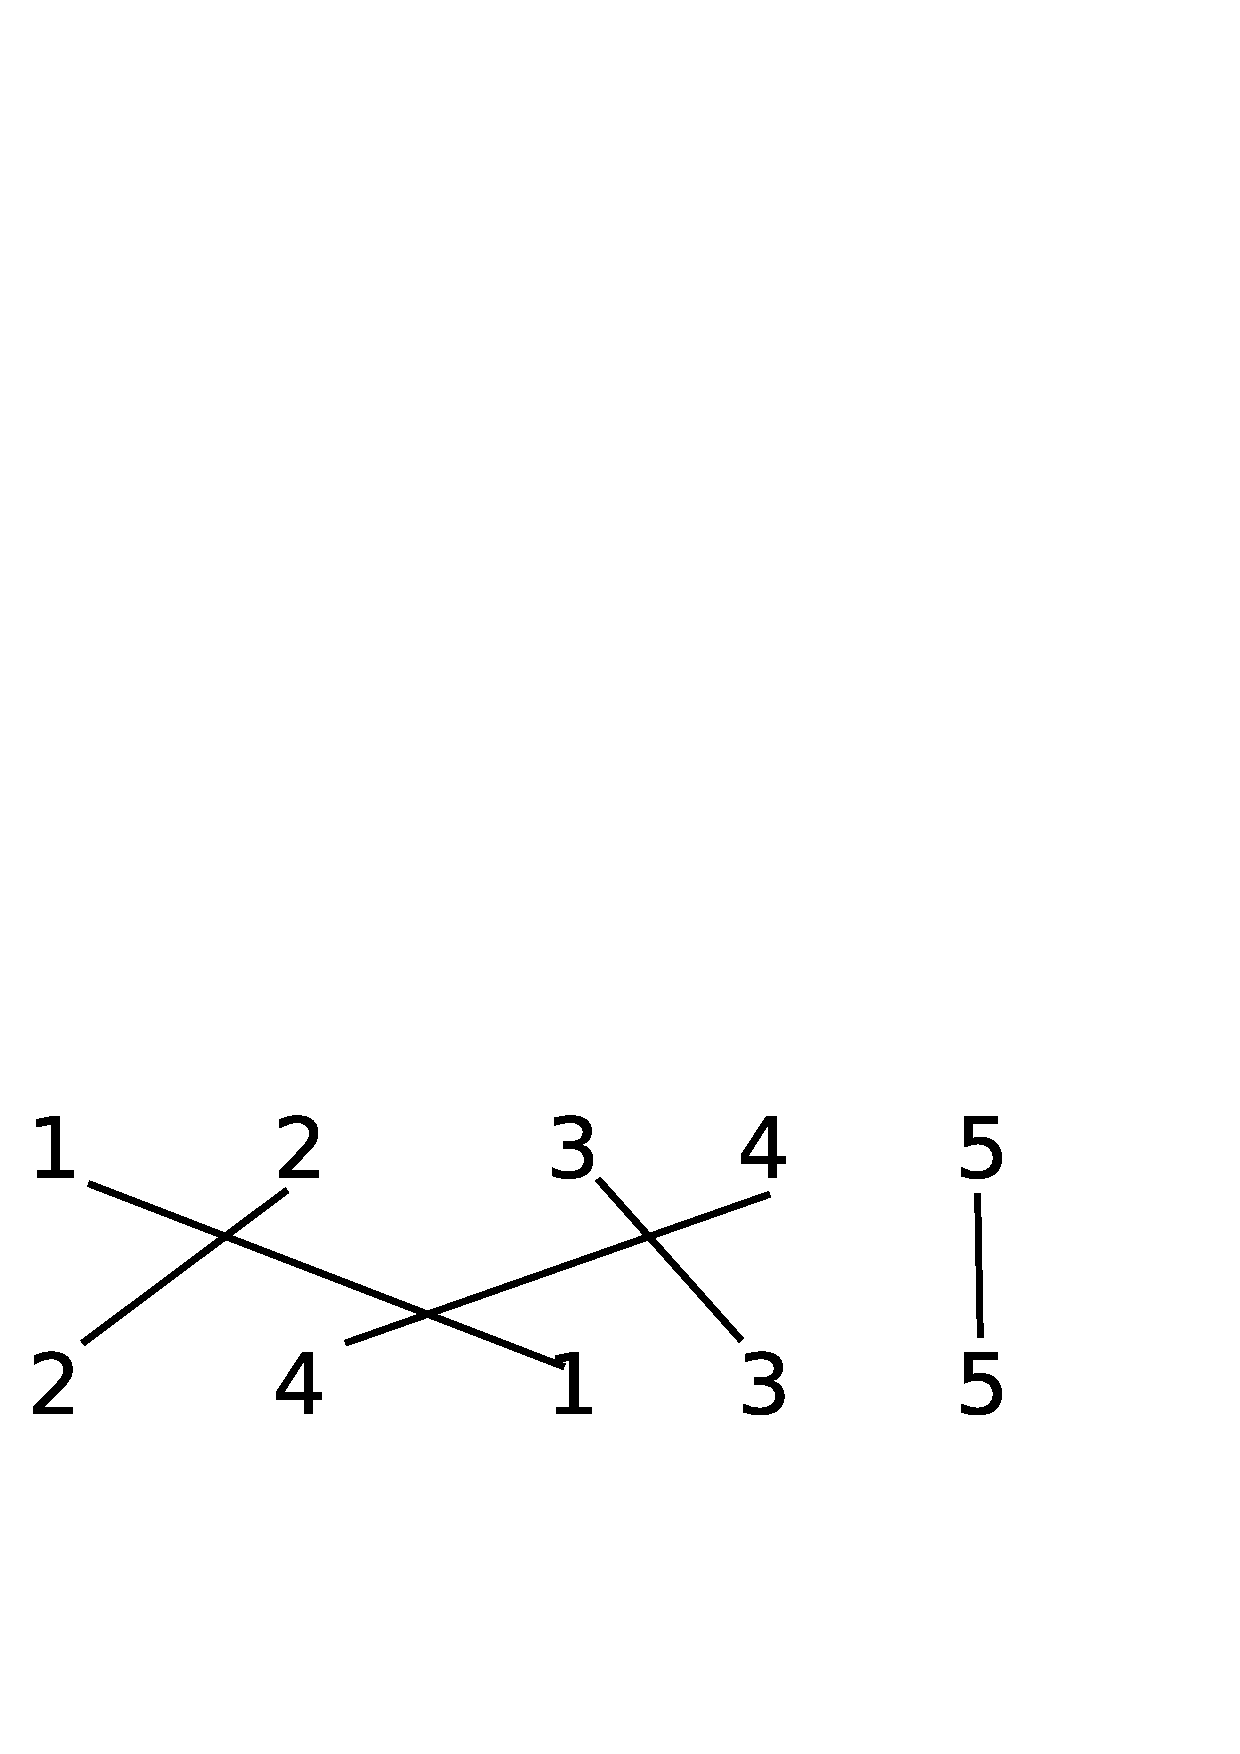
\includegraphics[width=2in] {L5-counting-inversion.png}
\end{figure}

}

\frame{
	\frametitle{Application 1: Genome comparison} 
\begin{figure}
 \includegraphics[width=3in] {L5-genome-comparison.png}
 \caption{Sequence comparison of the 5' flanking regions of mouse, rat and human ER$\beta$. } 
\end{figure}
{\small Reference: In vivo function of the 5' flanking region of mouse estrogen receptor $\beta$ gene, The Journal of Steroid Biochemistry and Molecular Biology Volume 105, Issues 1-5, June-July 2007, pages 57-62. }
} 

\frame{
	\frametitle{Application 2: A measure of bivariate association}
	\begin{itemize}
		\item Motivation: how to measure the association between two genes when given expression levels across $n$ time points? 
		\item Existing measures: 
			\begin{itemize}
				\item Linear relationship: Pearson's CC (most widely used, but sensitive to outliers)
				\item Monotonic relationship: Spearman, Kendall's correlation
				\item General statistical dependence: Renyi correlation, mutual information, maximal information coefficient
			\end{itemize}

		\item A novel measure:
			 \begin{center} 
			 $W_1 = \sum_{i=1}^{n-k+1} (I_i^+ + I_{i}^{-})$ 
			\end{center}
						Here,  $I_i^+$ is 1 if $X_{[i,..,i+k-1]}$ and $Y_{[i,..,i+k-1]}$ has the same order and $0$ otherwise, while $I_i^-$ is 1 if $X_{[i,..,i+k-1]}$ and $-Y_{[i,..,i+k-1]}$ has the same order and $0$ otherwise. 
		\item Advantage: 
			the association may exist across a subset of samples. For example, 
			\begin{center} 
$	X:\ 1\ 3\ 4\ 2\ 5$\\

$	Y:\ 1\ 4\ 5\ 2\ 3$
\end{center}
		
	$W_1 = 2$ when $k=3$. Much better than Pearson CC, et al. 
	\end{itemize}
	
	\begin{tiny}
		Ref: R. Wang, M. Waterman, H. Huang, PNAS, 2014
	\end{tiny}

}
 
\frame{
\frametitle{{\sc CountingInversion} problem}
\begin{itemize}
 \item 
 Solution: index pairs. The possible solution space has a size of $O(n^{2})$. 
\item Brute-force: $O(n^2)$ (Examining all index pairs $(i, j)$). \\
\item Can we design a better algorithm? 

 \end{itemize} 
} 

\frame{
\frametitle{{\sc CountingInversion} problem}
\begin{itemize}
\item 
{\sc Divide and Conquer} technique: 
\begin{enumerate}
 \item \textcolor{blue}{\bf Divide:} Divide $A$ into two arrays $A[0..{\lceil\frac{n}{2}\rceil}-1]$ and $A[{\lceil\frac{n}{2}\rceil}..n-1]$; thus counting inversions within $A[0..{\lceil\frac{n}{2}\rceil}-1]$ and $A[{\lceil\frac{n}{2}\rceil}..n-1]$ constitutes two subproblems. 
 \item \textcolor{blue}{\bf Conquer:} Counting inversions  within each half by calling {\sc CountingInversion} itself. 
% \item \textcolor{blue}{\bf Combine:} how to count inversion ($a_i$,$a_j$), when \textcolor{red}{ $a_i$ and $a_j$ are in different half?} \\
%       We will get a $O(n\log n)$ algorithm if we can perform {\bf combine} step in $O(n)$ time. 
\end{enumerate}
\end{itemize}

\begin{figure}
    
\begin{tikzpicture}[scale=1., auto,swap]
 
  \foreach \i/\name in { 0/5,1/2,2/3,3/1,4/7, 5/8, 6/6, 7/4 } {
         \draw[  fill=white, thick ] (\i*0.5,0) rectangle (\i*0.5+0.5, 0.5);
         \node at (\i*0.5+0.25, 0.5/2) {$\name$};
 }
 

 %level 2
  
   \foreach \i/\name\n in { 0/5/s2,1/2/s5,2/3/s5,3/1/s1 } {
         \draw[  fill=white, thick ] (\i*0.5-1,0-1) rectangle (\i*0.5-1+0.5, 0.5-1);
         \node (\n) at (\i*0.5+0.25-1, 0.5/2-1) {$\name$};
 }
 
    \foreach \i/\name/\n in { 4/7/s7, 5/8/s4, 6/6/s6, 7/4/s8 } {
         \draw[  fill=white, thick ] (\i*0.5+1,0-1) rectangle (\i*0.5+1+0.5, 0.5-1);
         \node (\n) at (\i*0.5+0.25+1, 0.5/2-1) {$\name$};
 }
 
  
 % lines 
 \foreach \source/\dest in {{( 4*0.5 , 0)/( 2*0.5 - 1, -0.5)}, {( 4*0.5 , 0)/( 6*0.5 + 1, -0.5)}} 
 	\path[draw=red, ->, thick]  \source  --  \dest;
 
	
  
\end{tikzpicture}

\end{figure}


%\begin{figure}
% 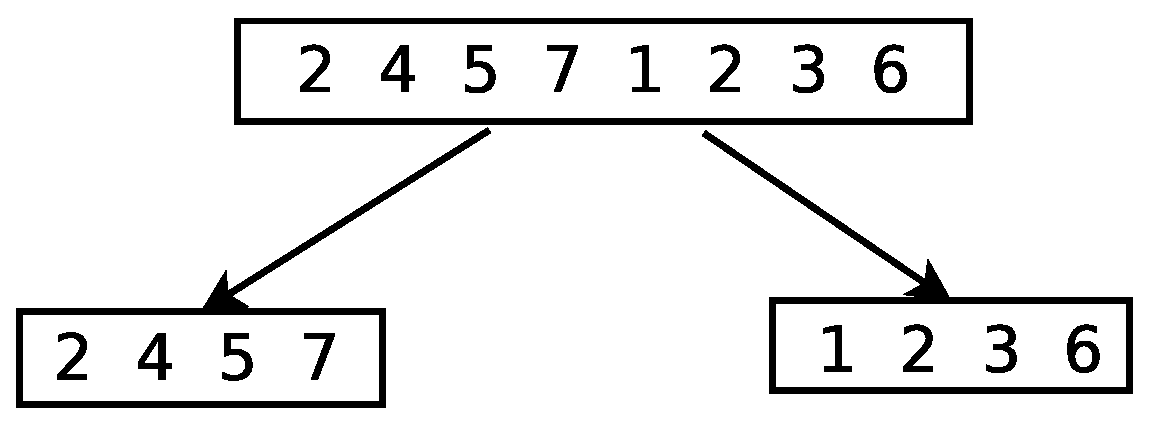
\includegraphics[width=2in] {L5-counting-inversion-example.eps}
%\end{figure}
}


\frame{
\frametitle{Combine strategy 1}

\begin{itemize}
    \item 
\textcolor{blue}{\bf Combine:} How to count the inversions ($i$,$j$) with $A[i]$ and $A[j]$ from different halves? \\
\item If the two halves $A[0..{\lceil\frac{n}{2}\rceil}-1]$ and $A[{\lceil\frac{n}{2}\rceil}..n-1]$ have no special structure, we have to examine all possible index pairs $i\in [0, {\lceil\frac{n}{2}\rceil}-1]$, $j\in [{\lceil\frac{n}{2}\rceil}, n-1]$ to count such inversions, which costs $\frac{n^2}{4}$ time. 
\item Thus, $T(n) = 2T(\frac{n}{2})  + \frac{n^2}{4} = O(n^2)$. 


\end{itemize}

\begin{figure}
    
\begin{tikzpicture}[scale=1., auto,swap]
 
  \foreach \i/\name in { 0/5,1/2,2/3,3/1,4/7, 5/8, 6/6, 7/4 } {
         \draw[  fill=white, thick ] (\i*0.5,0) rectangle (\i*0.5+0.5, 0.5);
         \node at (\i*0.5+0.25, 0.5/2) {$\name$};
 }

 %level 2
  
   \foreach \i/\name/\n in { 0/5/s2,1/2/s5,2/3/s3,3/1/s1} {
         \draw[  fill=white, thick ] (\i*0.5-1,0-1) rectangle (\i*0.5-1+0.5, 0.5-1);
         \node (\n) at (\i*0.5+0.25-1, 0.5/2-1) {$\name$};
 }
 
    \foreach \i/\name/\n in { 4/7/s7, 5/8/s4, 6/6/s6, 7/4/s8} {
         \draw[  fill=white, thick ] (\i*0.5+1,0-1) rectangle (\i*0.5+1+0.5, 0.5-1);
         \node (\n) at (\i*0.5+0.25+1, 0.5/2-1) {$\name$};
 }
 
  
 % lines 
 \foreach \source/\dest in {{( 4*0.5 , 0)/( 2*0.5 - 1, -0.5)}, {( 4*0.5 , 0)/( 6*0.5 + 1, -0.5)}} 
 	\path[draw=red, ->, thick]  \source  --  \dest;
 
\draw[green, dashed, thick] (s1.south) to [out=-30, in=180+30] (s7.south);
\draw[green, dashed, thick] (s1.south) to [out=-35, in=180+35] (s4.south);
\draw[green, dashed, thick] (s1.south) to [out=-40, in=180+40] (s6.south);
\draw[green, dashed, thick] (s1.south) to [out=-45, in=180+45] (s8.south);

\draw[green, dashed, thick] (s3.south) to [out=-35, in=180+35] (s7.south);
\draw[green, dashed, thick] (s3.south) to [out=-40, in=180+40] (s4.south);
\draw[green, dashed, thick] (s3.south) to [out=-45, in=180+45] (s6.south);
\draw[green, dashed, thick] (s3.south) to [out=-50, in=180+50] (s8.south);

\draw[green, dashed, thick] (s5.south) to [out=-40, in=180+40] (s7.south);
\draw[green, dashed, thick] (s5.south) to [out=-45, in=180+45] (s4.south);
\draw[green, dashed, thick] (s5.south) to [out=-50, in=180+50] (s6.south);
\draw[green, dashed, thick] (s5.south) to [out=-55, in=180+55] (s8.south);

\draw[green, dashed, thick] (s2.south) to [out=-45, in=180+45] (s7.south);
\draw[green, dashed, thick] (s2.south) to [out=-50, in=180+50] (s4.south);
\draw[green, dashed, thick] (s2.south) to [out=-55, in=180+55] (s6.south);
\draw[green, dashed, thick] (s2.south) to [out=-60, in=180+60] (s8.south);



\end{tikzpicture}

\end{figure}


}

\frame{
\frametitle{Combine strategy 2 }
\begin{itemize}
    \item 
\textcolor{blue}{\bf Combine:} How to count the inversions ($i$,$j$) with $A[i]$ and $A[j]$ from different halves? \\
%\item If the two halves $A[0..{\lceil\frac{n}{2}\rceil}-1]$ and $A[{\lceil\frac{n}{2}\rceil}..n-1]$ have no special structure, we have to examine all possible index pairs $i\in [0, {\lceil\frac{n}{2}\rceil}-1]$, $j\in [{\lceil\frac{n}{2}\rceil}, n-1]$ to count such inversions, which costs $\frac{n^2}{4}$ time.   Thus, $T(n) = 2T(\frac{n}{2})  + \frac{n^2}{4} = O(n^2)$. 

\item If the two halves are unstructured, it would be inefficient to count inversions. Thus,  we need to introduce some structures into $A[0..{\lceil\frac{n}{2}\rceil}-1]$ and $A[{\lceil\frac{n}{2}\rceil}..n-1]$. 
\item Note that it is relatively easy to count such inversions if \textcolor{red}{\bf elements in both halves  are in increasing order}.
\end{itemize}

\begin{figure}
    
\begin{tikzpicture}[scale=1., auto,swap]
 
  \foreach \i/\name in { 0/5,1/2,2/3,3/1,4/7, 5/8, 6/6, 7/4 } {
         \draw[  fill=white, thick ] (\i*0.5,0) rectangle (\i*0.5+0.5, 0.5);
         \node at (\i*0.5+0.25, 0.5/2) {$\name$};
 }

 %level 2
  
   \foreach \i/\name/\n in { 0/1/s1,1/2/s2,2/3/s3,3/5/s5} {
         \draw[  fill=white, thick ] (\i*0.5-1,0-1) rectangle (\i*0.5-1+0.5, 0.5-1);
         \node (\n) at (\i*0.5+0.25-1, 0.5/2-1) {$\name$};
 }
 
    \foreach \i/\name/\n in { 4/4/s4, 5/6/s6, 6/7/s7, 7/8/s8} {
         \draw[  fill=white, thick ] (\i*0.5+1,0-1) rectangle (\i*0.5+1+0.5, 0.5-1);
         \node (\n) at (\i*0.5+0.25+1, 0.5/2-1) {$\name$};
 }
 
  
 % lines 
 \foreach \source/\dest in {{( 4*0.5 , 0)/( 2*0.5 - 1, -0.5)}, {( 4*0.5 , 0)/( 6*0.5 + 1, -0.5)}} 
 	\path[draw=red, ->, thick]  \source  --  \dest;
 
\draw[green, dashed, thick] (s5.south) to [out=-30, in=180+30] (s4.south);
\draw[green, dashed, thick] (s3.south) to [out=-35, in=180+35] (s4.south);
\draw[green, dashed, thick] (s2.south) to [out=-40, in=180+40] (s4.south);
\draw[green, dashed, thick] (s1.south) to [out=-45, in=180+45] (s4.south);

\draw[green, dashed, thick] (s5.south) to [out=-35, in=180+35] (s6.south);


\end{tikzpicture}

\end{figure}

(See a demo)
%
%\begin{figure}
%    
%\begin{tikzpicture}[scale=1., auto,swap]
% 
%  \foreach \i/\name in { 0/,1/,2/,3/ } {
%         \draw[  fill=blue!20, thick ] (\i*0.5,0) rectangle (\i*0.5+0.5, 0.5);
%         \node at (\i*0.5+0.25, 0.5/2) {$\name$};
% }
% 
%  \foreach \i/\name in { 4/A_k, 5/, 6/, 7/ } {
%         \draw[   thick ] (\i*0.5,0) rectangle (\i*0.5+0.5, 0.5);
%         \node[red] at (\i*0.5+0.25, 0.5/2) {$\name$};
% }
% 
%
% %level 2
%  
%   \foreach \i/\name in { 0/,1/,2/L_i,3/ } {
%         \draw[  fill=blue!20, thick ] (\i*0.5-1,0-1) rectangle (\i*0.5-1+0.5, 0.5-1);
%         \node[red] at (\i*0.5+0.25-1, 0.5/2-1) {$\name$};
% }
% 
%    \foreach \i/\name in { 4/, 5/, 6/R_j, 7/} {
%         \draw[  fill=blue!20, thick ] (\i*0.5+1,0-1) rectangle (\i*0.5+1+0.5, 0.5-1);
%         \node[red] at (\i*0.5+0.25+1, 0.5/2-1) {$\name$};
% }
%  
%
% % lines 
% \foreach \source/\dest in {{( 4*0.5 , 0)/( 2*0.5 - 1, -0.5)}, {( 4*0.5 , 0)/( 6*0.5 + 1, -0.5)}} 
% 	\path[draw=red, <-, thick]  \source  --  \dest;
% 
%\node[blue] at (-0, 0.5/2-1.5) {sorted $A[l..m]$, called $L$};
%\node[blue] at (4.7, 0.5/2-1.5) {sorted $A[m+1..r]$, called $R$};
%\node[blue] at (2, 0.75) { $A[0..k-1]$ is sorted};
%    
%\end{tikzpicture}
%\end{figure}


%\begin{figure}
% \includegraphics[width=3in] {L5-merge-algo.eps}
%\end{figure}
}

\frame{
\frametitle{{\sc Sort-and-Count} algorithm }

\begin{small} 
{\sc Sort-and-Count}$(A)$
\begin{algorithmic}[1]
\STATE Divide $A$ into two sub-sequences $L$ and $R$;
\STATE $(RC_L, L)$ = {\sc Sort-and-Count}$(L)$;
\STATE $(RC_R, R)$ = {\sc Sort-and-Count}$(R)$;
\STATE $(C, A)$ = {\sc Merge-and-Count}$(L,R)$;
\RETURN{$ (RC=RC_L+RC_R+C, A);$}
\end{algorithmic}
\end{small} 
Time complexity: $T(n)=2T(\tfrac{n}{2}) + O(n) = O(n\log n)$. 
} 

\frame{
	\frametitle{ {\sc Merge-and-Count} algorithm} 
\begin{small} 

{\sc Merge-and-Count} $(L,R)$
\begin{algorithmic}[1]
\STATE $RC = 0;$ $ i=0; $ $j=0;$
\FOR{ $k=0$ to $\|L\|+\|R\|-1$ }
	\IF { $L[i] > R[j] $}
		\STATE $A[k] = R[j];$
		\STATE $j++;$
		\STATE \textcolor{red}{\bf $RC += (\|L\| - i);$}
		\IF{all elements in $R$ have been copied}
			\STATE{Copy the remainder elements from $L$ into $A$;}
			\STATE{break;}
		\ENDIF
	\ELSE 
		\STATE $A[k] = L[i];$
		\STATE $i++;$
		\IF{all elements in $L$ have been copied}
			\STATE{Copy the remainder elements from $R$ into $A$;}
			\STATE{break;}
		\ENDIF
	\ENDIF
\ENDFOR
\RETURN{($RC$, $A$); }
\end{algorithmic}

\end{small} 
}


%\frame{
%	\frametitle{Another view point} 
%	
%	\begin{itemize}
%		\item A sorted array has an inversion number of $0$.
%		\item Thus, we can treat the sorting process as a process to decrease inversion number to $0$.  
%		\item Suppose we can record the decrement of inversion number during the sorting process, the sum will be the inversion number. 
%	\end{itemize}
%
%
%}


\frame{
\begin{block}{}
{\sc QuickSort} algorithm: divide based on \textcolor{red}{\bf value of elements}  
\end{block}
}

\frame{
\frametitle{{\sc QuickSort} algorithm [C. A. R. Hoare, 1962] } 
\begin{figure}
 \includegraphics[width=1.7in] {L5-Hoare.jpg}
 \caption{Sir Charles Antony Richard Hoare, 2011}
\end{figure}

}

\frame{
\frametitle{{\sc QuickSort}: divide based on value of a randomly-selected element} 

\begin{footnotesize}
{\sc QuickSort}$(A)$ 
\begin{algorithmic}[1]
\STATE{$S_{-}=\{\}; S_{+}=\{\};$}
\STATE Choose a pivot $A[j]$ \textcolor{red}{\bf uniformly at random};
\FOR { $i=0 $ to $n-1$ }
	\STATE Put $A[i]$ in $S_{-}$ if $A[i] < A[j]$;
	\STATE Put $A[i]$ in $S_{+}$ if $A[i] \geq A[j]$;
\ENDFOR
\STATE {\sc QuickSort}$(S_{+});$
\STATE {\sc QuickSort}$(S_{-});$
\STATE Output $S_{-}$, then $A[j]$, then $S_{+}$; 
\end{algorithmic}
\end{footnotesize}

\begin{itemize}
    \item 
The randomization operation makes this algorithm \textcolor{red}{\bf simple} (relative to {\sc MergeSort} algorithm) but \textcolor{red}{\bf efficient}. 
\item However, the randomization also makes it difficult to analyze time-complexity: When dividing based on indices, it is easy to divide into two halves with equal size; in contrast, we divide based on value of a randomly-selected pivot and thus we cannot guarantee that each sub-problem has  exactly $\frac{n}{2}$ elements. 
\end{itemize}
}

\frame{
\frametitle{ Various cases of the execution of {\sc QuickSort} algorithm}



\begin{itemize}
 \item 
\textcolor{blue}{\bf Worst case:} selecting the smallest/largest element at each iteration. The subproblems decrease \textcolor{red}{\bf linearly} in size. 


\begin{center}
$T(n) = T(n-1) + O(n) = O(n^2)$
\end{center}

\ \\
\item 
\textcolor{blue}{\bf Best case:} select the median exactly at each iteration. The subproblems decrease \textcolor{red}{\bf exponentially} in size. 

\begin{center}
$T(n) = 2T(\tfrac{n}{2}) + O(n) = O(n \log n)$
\end{center}

\ \\
\item 
\textcolor{blue}{\bf Most cases:} instead of selecting the median exactly, we can select a \textcolor{red}{\bf nearly-central pivot} with high probability. 
We claim that the expected running time  is still 
\begin{center}
$T(n) = O(n \log n)$.
\end{center}

%$T(n) \leq T(n/4) + T(3/4 n) + cn \Rightarrow T(n) = O(n \log n)$. \\


\end{itemize}
}

\frame{
\frametitle{Analysis}

\begin{itemize}
\item Let $X$ denote the number of comparisons performed in line 4 and 5. After expanding all recursive calls, it is obvious that the running time of {\sc QuickSort} is $O( n + X)$. Our objective is to calculate $E[X]$. 
\item For simplicity, we represent each element using its
index in the sorted array, denoted as $\tilde{A}$. We have two key observations:  

	\item \textcolor{blue}{\bf Observation 1:} Any two elements $\tilde{A}[i]$ and $\tilde{A}[j]$ are compared at most once. 

%\begin{figure}
%  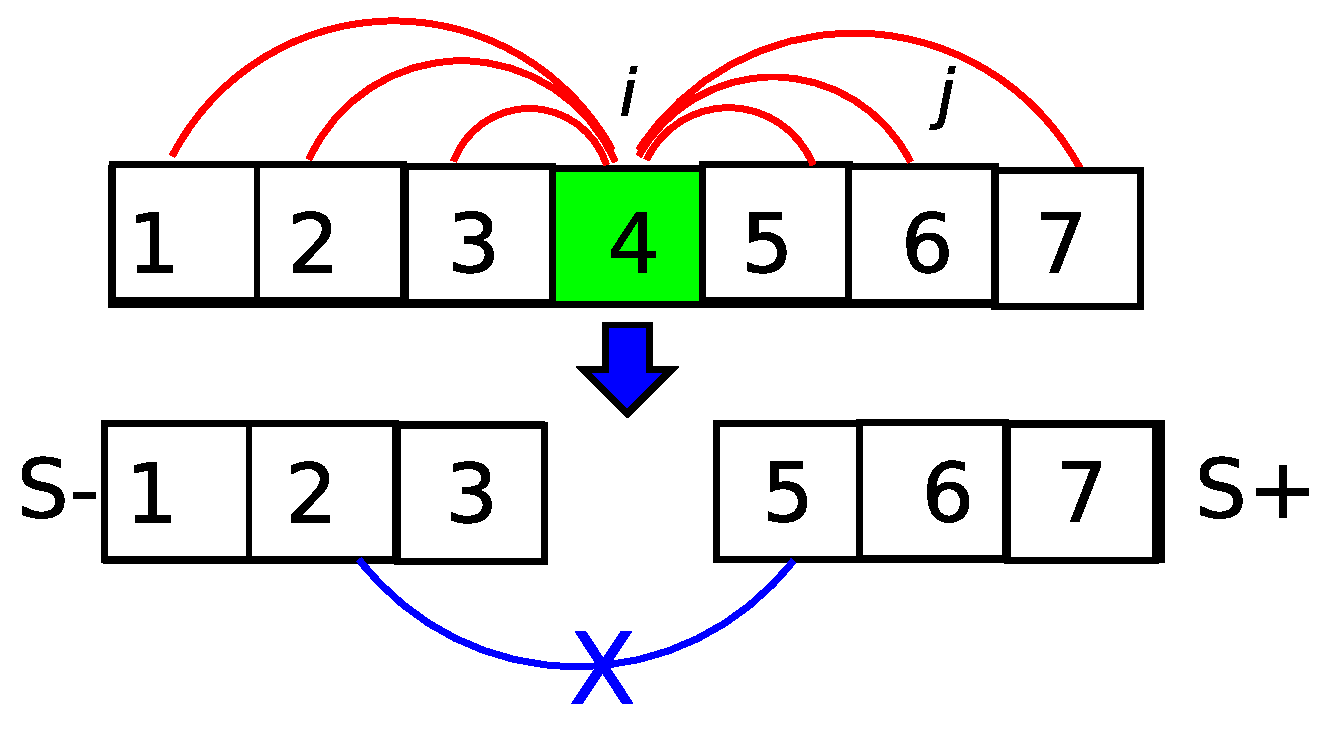
\includegraphics[width=1.8in]{L5-randomizedquicksort.eps}
%\end{figure}
\end{itemize} 

\begin{figure}
\begin{tikzpicture}[scale=1., auto,swap]
 
  \foreach \i/\name in { 0/1,1/2,2/3,3/4,4/5, 5/6, 6/7} {
         \draw[  fill=white, thick ]  (\i*0.5,0) rectangle (\i*0.5+0.5, 0.5);
         \node (U\name) at (\i*0.5+0.25, 0.5/2 ) {$\name$};
 }

 
   \foreach \i/\name in { 3/4} {
         \draw[  fill=green, thick ]  (\i*0.5,0) rectangle (\i*0.5+0.5, 0.5);
         \node (U\name) at (\i*0.5+0.25, 0.5/2 ) {$\name$};
 }
 
 %level 2
  
   \foreach \i/\name in { 0/1,1/2,2/3 } {
         \draw[  fill=white, thick ]  (\i*0.5 ,0-1.5) rectangle (\i*0.5 +0.5, 0.5-1.5);
         \node (B\name) at (\i*0.5+0.25 , 0.5/2-1.5) {$\name$};
 }
 
    \foreach \i/\name in { 4/5, 5/6, 6/7 } {
         \draw[  fill=white, thick ]   (\i*0.5  ,0-1.5) rectangle (\i*0.5 +0.5, 0.5-1.5);
         \node (B\name) at (\i*0.5+0.25 , 0.5/2-1.5) {$\name$};
 }
 %arrow
 \draw[blue, -latex, line width=3pt] (4*0.5-0.25, -0.2) -- (4*0.5-0.25, -0.9);
  %arc
  \draw[red, thick] (U4.north) to [out=60,in=180-60] (U5.north);
  \draw[red, thick] (U4.north) to [out=70,in=180-70] (U6.north);
  \draw[red, thick] (U4.north) to [out=80,in=180-80] (U7.north);	
  
    \draw[red, thick] (U4.north) to [out=180-60,in=60] (U3.north);
  \draw[red, thick] (U4.north) to [out=180-70,in=70] (U2.north);
  \draw[red, thick] (U4.north) to [out=180-80,in=80] (U1.north);	
  
    \draw[blue, thick] (B2.south) to [out=-80,in=260] (B6.south);	
    
   %no comparison 
   \node[red, thick] at (4*0.5-0.25, -2.1) {\bf X};
    \node[red, thick] at (4*0.5-0.25, 1) {$i$};
      \node[red, thick] at (7*0.5-0.25, 1) {$j$};

     \node[ thick] at (-0.6, -1.25) {$S_{-}$};
     \node[ thick] at (7*0.5 + 0.4, -1.25) {$S_{+}$};
     \node[ thick] at (-0.6, 0.25 ) {$\tilde{A}$};

\end{tikzpicture}

\end{figure}


} 

\frame{
\frametitle{Analysis cont'd}

\begin{figure}
    
\begin{tikzpicture}[scale=0.78, auto,swap]
 
  \foreach \i/\name in { 0/1,1/2,2/3,3/4,4/5, 5/6, 6/7} {
         \draw[  fill=white, thick ]  (\i*0.5,0) rectangle (\i*0.5+0.5, 0.5);
         \node (U\name) at (\i*0.5+0.25, 0.5/2 ) {$\name$};
 }

 
   \foreach \i/\name in { 3/4} {
         \draw[  fill=green, thick ]  (\i*0.5,0) rectangle (\i*0.5+0.5, 0.5);
         \node (U\name) at (\i*0.5+0.25, 0.5/2 ) {$\name$};
 }
 
 %level 2
  
   \foreach \i/\name in { 0/1,1/2,2/3 } {
         \draw[  fill=white, thick ]  (\i*0.5 ,0-1.5) rectangle (\i*0.5 +0.5, 0.5-1.5);
         \node (B\name) at (\i*0.5+0.25 , 0.5/2-1.5) {$\name$};
 }
 
    \foreach \i/\name in { 4/5, 5/6, 6/7 } {
         \draw[  fill=white, thick ]   (\i*0.5  ,0-1.5) rectangle (\i*0.5 +0.5, 0.5-1.5);
         \node (B\name) at (\i*0.5+0.25 , 0.5/2-1.5) {$\name$};
 }
 %arrow
 \draw[blue, -latex, line width=3pt] (4*0.5-0.25, -0.2) -- (4*0.5-0.25, -0.9);
  %arc
  \draw[red, thick] (U4.north) to [out=60,in=180-60] (U5.north);
  \draw[red, thick] (U4.north) to [out=70,in=180-70] (U6.north);
  \draw[red, thick] (U4.north) to [out=80,in=180-80] (U7.north);	
  
    \draw[red, thick] (U4.north) to [out=180-60,in=60] (U3.north);
  \draw[red, thick] (U4.north) to [out=180-70,in=70] (U2.north);
  \draw[red, thick] (U4.north) to [out=180-80,in=80] (U1.north);	
  
    \draw[blue, thick] (B2.south) to [out=-80,in=260] (B6.south);	
    
   %no comparison 
   \node[red, thick] at (4*0.5-0.25, -2.1) {\bf X};
    \node[red, thick] at (4*0.5-0.25, 1) {$i$};
      \node[red, thick] at (7*0.5-0.25, 1) {$j$};

     \node[ thick] at (-0.6, -1.25) {$S_{-}$};
     \node[ thick] at (7*0.5 + 0.4, -1.25) {$S_{+}$};
     \node[ thick] at (-0.6, 0.25 ) {$\tilde{A}$};

\end{tikzpicture}

\end{figure}



%\begin{figure}
%  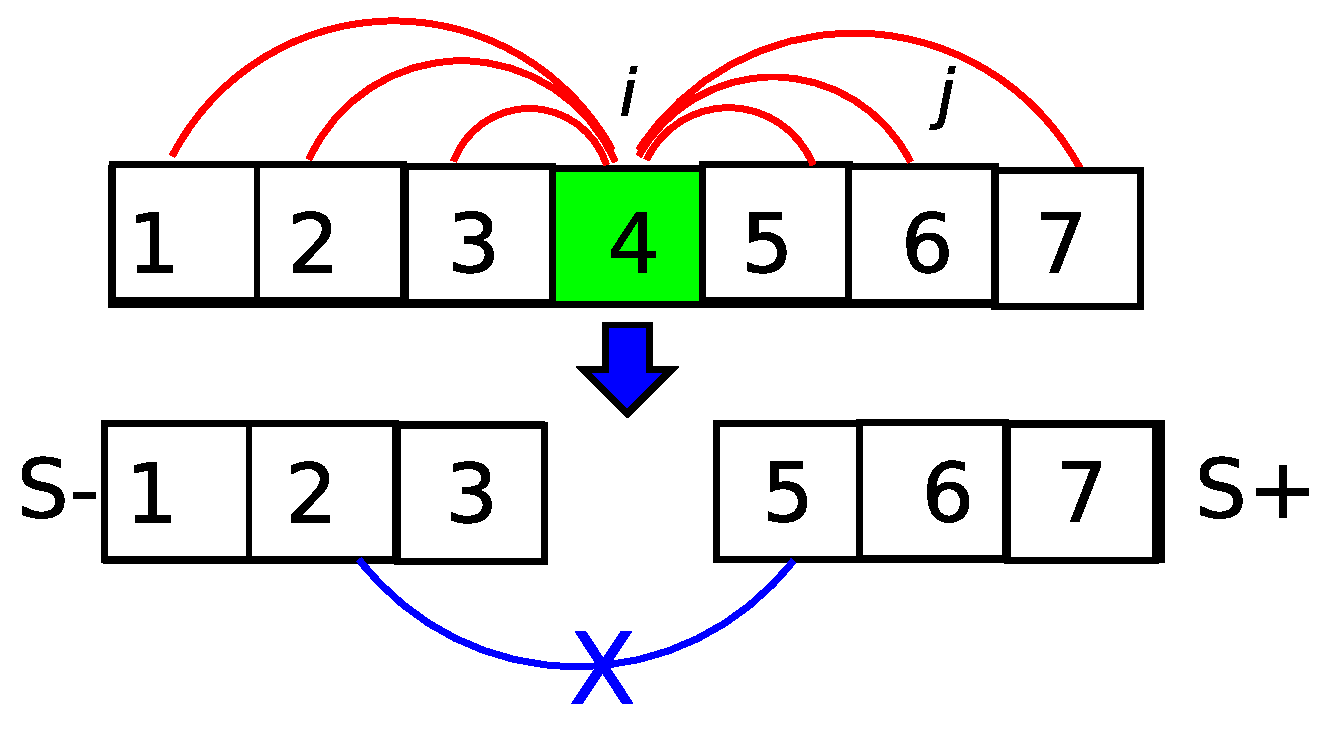
\includegraphics[width=1.8in]{L5-randomizedquicksort.eps}
%\end{figure}

\begin{itemize}

      \item Define index variable $X_{ij} = \begin{cases} 
      1 & \text{ if } \tilde{A}[i] \text{ is compared with } \tilde{A}[j] \nonumber \\
      0 & \text{ otherwise } \nonumber
      \end{cases} $
      \item Thus  $X = \sum\nolimits_{i=0}^{n-1}\sum\nolimits_{j=i+1}^{n-1} X_{ij}$. 
      \begin{eqnarray}
      E[ X ] & = &  E [\sum\nolimits_{i=0}^{n-1}\sum\nolimits_{j=i+1}^{n-1} X_{ij} ] \nonumber \\
              & = &   \sum\nolimits_{i=0}^{n-1}\sum\nolimits_{j=i+1}^{n-1} E[ X_{ij} ] \nonumber \\
              & = &   \sum\nolimits_{i=0}^{n-1}\sum\nolimits_{j=i+1}^{n-1} \Pr( \tilde{A}[i]  \text{ is compared with } \tilde{A}[j] )  \nonumber 
      \end{eqnarray} 

\end{itemize} 
}

\frame{
\frametitle{Analysis  cont'd}

\begin{itemize}
\item \textcolor{blue}{\bf Observation 2:} $\tilde{A}[i]$ and $\tilde{A}[j]$ are compared iff either $\tilde{A}[i]$ or $\tilde{A}[j]$ is selected as pivot when processing elements containing $\tilde{A}[i..j]$.  
      \item We claim $\Pr( \tilde{A}[i]  \text{ is compared with } \tilde{A}[j] )  = \frac{2}{j-i+1}$. (Why?) 
      \item Then
      \begin{eqnarray}
      E[ X ]        & = &   \sum\nolimits_{i=0}^{n-1}\sum\nolimits_{j=i+1}^{n-1} \Pr( \tilde{A}[i]  \text{ is compared with } \tilde{A}[j])  \nonumber \\
      & = &  \sum\nolimits_{i=0}^{n-1}\sum\nolimits_{j=i+1}^{n-1}  \frac{2}{j-i+1} \nonumber \\ 
      & = & \sum\nolimits_{i=0}^{n-1} \sum\nolimits_{k=1}^{n-i-1} \frac{2}{k+1}  \nonumber \\        
      & \leq & \sum\nolimits_{i=0}^{n-1} \sum\nolimits_{k=1}^{n-1} \frac{2}{k+1} \nonumber \\
      & = & O( n \log n ) \nonumber 
      \end{eqnarray} 
      \item Here $k$ is defined as $ k=j-i$.
\end{itemize} 

}


\frame{
	\frametitle{Why $\Pr( \tilde{A}[i]  \text{ is compared with } \tilde{A}[j] )  = \frac{2}{j-i+1}$? }
	
\begin{figure}
    
\begin{tikzpicture}[scale=0.78, auto,swap]
 
 %level 1
 \def\dx{0}
 \def\dy{0};

  \node[ultra thick] at ( - 0.5 + \dx, 0.25 + \dy) {$\tilde{A}$};

  \foreach \i/\name in { 0/1,1/2, 2/3} {
         \draw[  fill=white, thick ]  (\i*0.5 + \dx,0 + \dy) rectangle (\i*0.5+0.5 + \dx, 0.5 + \dy);
         \node (U\name) at (\i*0.5+0.25+ \dx, 0.5/2 + \dy) {$\name$};
 }
 
 \foreach \i/\name in { 0/1} {
         \node[ultra thick, red] at (\i*0.5+0.25+ \dx, 0.5/2 + \dy + 0.5) {$i$};
 }

 \foreach \i/\name in { 2/3} {
         \node[ultra thick, red] at (\i*0.5+0.25+ \dx, 0.5/2 + \dy + 0.5) {$j$};
 }
 
  \node[ultra thick, blue] at (0.5+0.25 - 3.5, 0.5/2 - 1 + 0.5) {Pivot:};
 
 %arrow 
     \draw[->,  thick, blue] ( 1*0.5 + 0.25+ \dx, 0.5/2 + \dy - 0.5) -- node[left, below]{\small $1$} (1*0.5 + 0.25+ \dx - 3, 0.5/2 + \dy - 2 + 0.8); 

      \draw[->,  thick, blue] ( 1*0.5 + 0.25+ \dx, 0.5/2 + \dy - 0.5) -- node[right]{\small $2$} (1*0.5 + 0.25+ \dx , 0.5/2 + \dy - 2 + 0.8); 

     \draw[->,  thick, blue] ( 1*0.5 + 0.25+ \dx, 0.5/2 + \dy - 0.5) -- node[right, below]{\small $3$} (1*0.5 + 0.25+ \dx + 3, 0.5/2 + \dy - 2 + 0.8); 

 
 %level 2 
 %1 
 \def\dx{-3}
 \def\dy{-2};
  \foreach \i/\name in { 0/1,1/2,2/3} {
         \draw[  fill=white, thick ]  (\i*0.5 + \dx,0 + \dy) rectangle (\i*0.5+0.5 + \dx, 0.5 + \dy);
         \node (U\name) at (\i*0.5+0.25+ \dx, 0.5/2 + \dy) {$\name$};
 }

   \foreach \i/\name in { 0/1} {
         \draw[  fill=green, thick ]  (\i*0.5 + \dx,0 + \dy) rectangle (\i*0.5+0.5 + \dx, 0.5 + \dy);
         \node (U\name) at (\i*0.5+0.25 + \dx, 0.5/2 + \dy) {$\name$};
 }

  %arc
    \draw[red, thick] (U3.north) to [out=180-70,in=70] (U1.north);


 %2 
 \def\dx{0}
 \def\dy{-2};
  \foreach \i/\name in { 0/1,1/2,2/3} {
         \draw[  fill=white, thick ]  (\i*0.5 + \dx,0 + \dy) rectangle (\i*0.5+0.5 + \dx, 0.5 + \dy);
         \node (U\name) at (\i*0.5+0.25+ \dx, 0.5/2 + \dy) {$\name$};
 }

   \foreach \i/\name in { 1/2} {
         \draw[  fill=green, thick ]  (\i*0.5 + \dx,0 + \dy) rectangle (\i*0.5+0.5 + \dx, 0.5 + \dy);
         \node (U\name) at (\i*0.5+0.25 + \dx, 0.5/2 + \dy) {$\name$};
 }

  %arc
 %   \draw[red, thick] (U3.north) to [out=180-70,in=70] (U1.north);


 %3 
 \def\dx{+3}
 \def\dy{-2};
  \foreach \i/\name in { 0/1,1/2,2/3} {
         \draw[  fill=white, thick ]  (\i*0.5 + \dx,0 + \dy) rectangle (\i*0.5+0.5 + \dx, 0.5 + \dy);
         \node (U\name) at (\i*0.5+0.25+ \dx, 0.5/2 + \dy) {$\name$};
 }

   \foreach \i/\name in { 2/3} {
         \draw[  fill=green, thick ]  (\i*0.5 + \dx,0 + \dy) rectangle (\i*0.5+0.5 + \dx, 0.5 + \dy);
         \node (U\name) at (\i*0.5+0.25 + \dx, 0.5/2 + \dy) {$\name$};
 }

  %arc
    \draw[red, thick] (U3.north) to [out=180-70,in=70] (U1.north);


%  \draw[red, thick] (U4.north) to [out=60,in=180-60] (U5.north);
%  \draw[red, thick] (U4.north) to [out=70,in=180-70] (U6.north);
%  \draw[red, thick] (U4.north) to [out=80,in=180-80] (U7.north);	
%  
%    \draw[red, thick] (U4.north) to [out=180-60,in=60] (U3.north);
%  \draw[red, thick] (U4.north) to [out=180-70,in=70] (U2.north);
%  \draw[red, thick] (U4.north) to [out=180-80,in=80] (U1.north);	
  



\end{tikzpicture}

\end{figure}

\begin{itemize}
	\item Let's examine a simple example first: For an array with only 3 elements, each element will be selected as pivot with equal probability $\tfrac{1}{3}$. 
	\item In two out of the three cases, ${\tilde{A}[i]}$ is compared with ${\tilde{A}[j]}$. Hence, 
	$\Pr( {\tilde{A}[i]}  \text{ is compared with } {\tilde{A}[j]} )  =  \frac{2}{3}$
\end{itemize}
}



\frame{
	\frametitle{Why $\Pr( \tilde{A}[i]  \text{ is compared with } \tilde{A}[j] )  = \frac{2}{j-i+1}$? cont`d}
	
\begin{figure}
    
\begin{tikzpicture}[scale=0.75, auto,swap]
 
 %level 1
 \def\dx{0}
 \def\dy{0};
 
   \node[ultra thick] at ( - 0.5 + \dx -0.25, 0.25 + \dy) {$\tilde{A}$};

 
  \foreach \i/\name in { 0/1,1/2, 2/3, 3/4} {
         \draw[  fill=white, thick ]  (\i*0.5 + \dx -0.25,0 + \dy) rectangle (\i*0.5+0.5 + \dx - 0.25, 0.5 + \dy);
         \node (U\name) at (\i*0.5+0.25+ \dx -0.25, 0.5/2 + \dy) {$\name$};
 }
 
 \foreach \i/\name in { 0/1} {
         \node[ultra thick, red] at (\i*0.5+0.25+ \dx -0.25, 0.5/2 + \dy + 0.5) {$i$};
 }

 \foreach \i/\name in { 2/3} {
         \node[ultra thick, red] at (\i*0.5+0.25+ \dx -0.25, 0.5/2 + \dy + 0.5) {$j$};
 }
 
  \node[ultra thick, blue] at (0.5+0.25 - 5, 0.5/2 - 1 + 0.5) {Pivot:};
 
 %arrow 
     \draw[->,  thick, blue] ( 1*0.5 + 0.25+ \dx, 0.5/2 + \dy - 0.5) -- node[left, above]{\small $1$} (1*0.5 + 0.25+ \dx - 6, 0.5/2 + \dy - 2 + 0.8); 

     \draw[->,  thick, blue] ( 1*0.5 + 0.25+ \dx, 0.5/2 + \dy - 0.5) -- node[left, below]{\small $2$} (1*0.5 + 0.25+ \dx - 2, 0.5/2 + \dy - 2 + 0.8); 

     \draw[->,  thick, blue] ( 1*0.5 + 0.25+ \dx, 0.5/2 + \dy - 0.5) -- node[right, below]{\small $3$} (1*0.5 + 0.25+ \dx + 2, 0.5/2 + \dy - 2 + 0.8); 

     \draw[->,  thick, blue] ( 1*0.5 + 0.25+ \dx, 0.5/2 + \dy - 0.5) -- node[right, above]{\small $4$} (1*0.5 + 0.25+ \dx + 6, 0.5/2 + \dy - 2 + 0.8); 


 
 %level 2 
 %1 
 \def\dx{-6}
 \def\dy{-2};
  \foreach \i/\name in { 0/1,1/2,2/3, 3/4} {
         \draw[  fill=white, thick ]  (\i*0.5 + \dx,0 + \dy) rectangle (\i*0.5+0.5 + \dx, 0.5 + \dy);
         \node (U\name) at (\i*0.5+0.25+ \dx, 0.5/2 + \dy) {$\name$};
 }

   \foreach \i/\name in { 0/1} {
         \draw[  fill=green, thick ]  (\i*0.5 + \dx,0 + \dy) rectangle (\i*0.5+0.5 + \dx, 0.5 + \dy);
         \node (U\name) at (\i*0.5+0.25 + \dx, 0.5/2 + \dy) {$\name$};
 }

  %arc
    \draw[red, thick] (U3.north) to [out=180-70,in=70] (U1.north);


 %2 
 \def\dx{-2}
 \def\dy{-2};
  \foreach \i/\name in { 0/1,1/2,2/3, 3/4} {
         \draw[  fill=white, thick ]  (\i*0.5 + \dx,0 + \dy) rectangle (\i*0.5+0.5 + \dx, 0.5 + \dy);
         \node (U\name) at (\i*0.5+0.25+ \dx, 0.5/2 + \dy) {$\name$};
 }

   \foreach \i/\name in { 1/2} {
         \draw[  fill=green, thick ]  (\i*0.5 + \dx,0 + \dy) rectangle (\i*0.5+0.5 + \dx, 0.5 + \dy);
         \node (U\name) at (\i*0.5+0.25 + \dx, 0.5/2 + \dy) {$\name$};
 }

  %arc
 %   \draw[red, thick] (U3.north) to [out=180-70,in=70] (U1.north);


 %3 
 \def\dx{+2}
 \def\dy{-2};
  \foreach \i/\name in { 0/1,1/2,2/3, 3/4} {
         \draw[  fill=white, thick ]  (\i*0.5 + \dx,0 + \dy) rectangle (\i*0.5+0.5 + \dx, 0.5 + \dy);
         \node (U\name) at (\i*0.5+0.25+ \dx, 0.5/2 + \dy) {$\name$};
 }

   \foreach \i/\name in { 2/3} {
         \draw[  fill=green, thick ]  (\i*0.5 + \dx,0 + \dy) rectangle (\i*0.5+0.5 + \dx, 0.5 + \dy);
         \node (U\name) at (\i*0.5+0.25 + \dx, 0.5/2 + \dy) {$\name$};
 }

  %arc
    \draw[red, thick] (U3.north) to [out=180-70,in=70] (U1.north);



 %4 
 \def\dx{+6}
 \def\dy{-2};
  \foreach \i/\name in { 0/1,1/2,2/3, 3/4} {
         \draw[  fill=white, thick ]  (\i*0.5 + \dx,0 + \dy) rectangle (\i*0.5+0.5 + \dx, 0.5 + \dy);
         \node (U\name) at (\i*0.5+0.25+ \dx, 0.5/2 + \dy) {$\name$};
 }

   \foreach \i/\name in { 3/4} {
         \draw[  fill=green, thick ]  (\i*0.5 + \dx,0 + \dy) rectangle (\i*0.5+0.5 + \dx, 0.5 + \dy);
         \node (U\name) at (\i*0.5+0.25 + \dx, 0.5/2 + \dy) {$\name$};
 }

  %arc
    \draw[red, thick] (U3.north) to [out=180-70,in=70] (U1.north);
%  \draw[red, thick] (U4.north) to [out=60,in=180-60] (U5.north);
%  \draw[red, thick] (U4.north) to [out=70,in=180-70] (U6.north);
%  \draw[red, thick] (U4.north) to [out=80,in=180-80] (U7.north);	
%  
%    \draw[red, thick] (U4.north) to [out=180-60,in=60] (U3.north);
%  \draw[red, thick] (U4.north) to [out=180-70,in=70] (U2.north);
%  \draw[red, thick] (U4.north) to [out=180-80,in=80] (U1.north);	
  



\end{tikzpicture}

\end{figure}


\begin{itemize}
	\item Let's  consider a larger  array with  4 elements. 
	\item Each element will be selected as pivot with equal probability $\tfrac{1}{4}$: the selection of  ${\tilde{A}[i]}$ or ${\tilde{A}[j]}$ as pivot will lead to an immediate comparison of ${\tilde{A}[i]}$ and ${\tilde{A}[j]}$. In contrast, the selection of  $\tilde{A}[3]$ as pivot produces a smaller problem, where ${\tilde{A}[i]}$ will be compared with ${\tilde{A}[j]}$ with  probability  $\frac{2}{3}$ by induction. Hence,  
	\begin{eqnarray}	
 \Pr( {\tilde{A}[i]}  \text{ is compared with } {\tilde{A}[j]} )  &=&  \tfrac{1}{4} + 0 + \tfrac{1}{4} + \tfrac{1}{4} \times  \tfrac{2}{3} \nonumber\\ 
 &=&  \tfrac{3}{4} \times  \tfrac{2}{3}  + \tfrac{1}{4} \times  \tfrac{2}{3} \nonumber\\
 &=&  \tfrac{2}{3}\nonumber
 	\end{eqnarray}

\end{itemize}
}


\frame{
	\frametitle{Why $\Pr( \tilde{A}[i]  \text{ is compared with } \tilde{A}[j] )  = \frac{2}{j-i+1}$? cont`d}
	
\begin{figure}
\begin{tikzpicture}[scale=1, auto,swap]
 
 %level 1
 \def\dx{0}
 \def\dy{0};
  \foreach \i/\name in { 0/1,1/2, 2/3, 3/4, 4/5, 5/6, 6/\dots, 7/n} {
         \draw[  fill=white, thick ]  (\i*0.5 + \dx,0 + \dy) rectangle (\i*0.5+0.5 + \dx, 0.5 + \dy);
         \node  at (\i*0.5+0.25+ \dx, 0.5/2 + \dy) {$\name$};
 }

 \def\dy{0.5}; 
   \foreach \i/\name in {  0/i, 2/j} {
          \node[red]  at (\i*0.5+0.25+ \dx, 0.5/2 + \dy) {$\name$};
 }
  
 \node[ultra thick]  at (0.25+ \dx - 0.8, 0.5/2 + \dy -0.5) {$\tilde{A}$};
 
 
\end{tikzpicture}
\end{figure}

\begin{itemize}
	\item Now let's extend these  observations to general case that $A$ has $n$ elements. By induction over the size of $A$, we can calculate the probability as: 
	\begin{eqnarray}	
 \Pr( \tilde{A}[i]  \text{ is compared with } \tilde{A}[j] )  &=&  \tfrac{1}{n} + \tfrac{1}{n} +  \tfrac{n-(j-i+1)}{n} \times  \tfrac{2}{j-i+1}  \nonumber\\ 
 &=&  (\tfrac{j-i+1}{n} +  \tfrac{n-(j-i+1)}{n}) \times  \tfrac{2}{j-i+1}   \nonumber\\
 &=&  \tfrac{2}{j-i+1}\nonumber
 	\end{eqnarray}
	
\end{itemize}

}


\frame{
	\frametitle{A special case:  neighbors should definitely compare with each other}
	
\begin{figure}
    
\begin{tikzpicture}[scale=0.78, auto,swap]
 
 %level 1
 \def\dx{0}
 \def\dy{0};

  \node[ultra thick] at ( - 0.5 + \dx, 0.25 + \dy) {$\tilde{A}$};

  \foreach \i/\name in { 0/1,1/2, 2/3} {
         \draw[  fill=white, thick ]  (\i*0.5 + \dx,0 + \dy) rectangle (\i*0.5+0.5 + \dx, 0.5 + \dy);
         \node (U\name) at (\i*0.5+0.25+ \dx, 0.5/2 + \dy) {$\name$};
 }
 
 \foreach \i/\name in { 0/1} {
         \node[ultra thick, red] at (\i*0.5+0.25+ \dx, 0.5/2 + \dy + 0.5) {$i$};
 }

 \foreach \i/\name in { 1/2} {
         \node[ultra thick, red] at (\i*0.5+0.25+ \dx, 0.5/2 + \dy + 0.5) {$j$};
 }
 
  \node[ultra thick, blue] at (0.5+0.25 - 3.5, 0.5/2 - 1 + 0.5) {Pivot:};
 
 %arrow 
     \draw[->,  thick, blue] ( 1*0.5 + 0.25+ \dx, 0.5/2 + \dy - 0.5) -- node[left, below]{\small $1$} (1*0.5 + 0.25+ \dx - 3, 0.5/2 + \dy - 2 + 0.8); 

      \draw[->,  thick, blue] ( 1*0.5 + 0.25+ \dx, 0.5/2 + \dy - 0.5) -- node[right]{\small $2$} (1*0.5 + 0.25+ \dx , 0.5/2 + \dy - 2 + 0.8); 

     \draw[->,  thick, blue] ( 1*0.5 + 0.25+ \dx, 0.5/2 + \dy - 0.5) -- node[right, below]{\small $3$} (1*0.5 + 0.25+ \dx + 3, 0.5/2 + \dy - 2 + 0.8); 

 
 %level 2 
 %1 
 \def\dx{-3}
 \def\dy{-2};
  \foreach \i/\name in { 0/1,1/2,2/3} {
         \draw[  fill=white, thick ]  (\i*0.5 + \dx,0 + \dy) rectangle (\i*0.5+0.5 + \dx, 0.5 + \dy);
         \node (U\name) at (\i*0.5+0.25+ \dx, 0.5/2 + \dy) {$\name$};
 }

   \foreach \i/\name in { 0/1} {
         \draw[  fill=green, thick ]  (\i*0.5 + \dx,0 + \dy) rectangle (\i*0.5+0.5 + \dx, 0.5 + \dy);
         \node (U\name) at (\i*0.5+0.25 + \dx, 0.5/2 + \dy) {$\name$};
 }

  %arc
    \draw[red, thick] (U2.north) to [out=180-70,in=70] (U1.north);


 %2 
 \def\dx{0}
 \def\dy{-2};
  \foreach \i/\name in { 0/1,1/2,2/3} {
         \draw[  fill=white, thick ]  (\i*0.5 + \dx,0 + \dy) rectangle (\i*0.5+0.5 + \dx, 0.5 + \dy);
         \node (U\name) at (\i*0.5+0.25+ \dx, 0.5/2 + \dy) {$\name$};
 }

   \foreach \i/\name in { 1/2} {
         \draw[  fill=green, thick ]  (\i*0.5 + \dx,0 + \dy) rectangle (\i*0.5+0.5 + \dx, 0.5 + \dy);
         \node (U\name) at (\i*0.5+0.25 + \dx, 0.5/2 + \dy) {$\name$};
 }

  %arc
    \draw[red, thick] (U2.north) to [out=180-70,in=70] (U1.north);


 %3 
 \def\dx{+3}
 \def\dy{-2};
  \foreach \i/\name in { 0/1,1/2,2/3} {
         \draw[  fill=white, thick ]  (\i*0.5 + \dx,0 + \dy) rectangle (\i*0.5+0.5 + \dx, 0.5 + \dy);
         \node (U\name) at (\i*0.5+0.25+ \dx, 0.5/2 + \dy) {$\name$};
 }

   \foreach \i/\name in { 2/3} {
         \draw[  fill=green, thick ]  (\i*0.5 + \dx,0 + \dy) rectangle (\i*0.5+0.5 + \dx, 0.5 + \dy);
         \node (U\name) at (\i*0.5+0.25 + \dx, 0.5/2 + \dy) {$\name$};
 }

  %arc
 %   \draw[red, thick] (U3.north) to [out=180-70,in=70] (U1.north);


%  \draw[red, thick] (U4.north) to [out=60,in=180-60] (U5.north);
%  \draw[red, thick] (U4.north) to [out=70,in=180-70] (U6.north);
%  \draw[red, thick] (U4.north) to [out=80,in=180-80] (U7.north);	
%  
%    \draw[red, thick] (U4.north) to [out=180-60,in=60] (U3.north);
%  \draw[red, thick] (U4.north) to [out=180-70,in=70] (U2.north);
%  \draw[red, thick] (U4.north) to [out=180-80,in=80] (U1.north);	
  



\end{tikzpicture}

\end{figure}

\begin{itemize}
	\item Let's examine a simple example first: For an array with only 3 elements, each element will be selected as pivot with equal probability $\tfrac{1}{3}$. 
	\item  
	$\Pr( {\tilde{A}[i]}  \text{ is compared with } {\tilde{A}[i+1]} )  =  \frac{1}{3}  + \frac{1}{3} + \frac{1}{3}\times 1 = 1$
\end{itemize}
}



\frame{
\frametitle{{\sc Modified QuickSort}: easier to analyze }
\begin{small}
{\sc ModifiedQuickSort}$(A)$
\begin{algorithmic}[1]
\WHILE{{\tt TRUE}}
	\STATE Choose a pivot $A[j]$ \textcolor{red}{\bf uniformly at random};
	\STATE{$S_{-}=\{\}; S_{+}=\{\};$}
	\FOR { $i=0 $ to $n-1$ }
		\STATE Put $A[i]$ in $S_{-}$ if $A[i] <  A[j]$;
		\STATE Put $A[i]$ in $S_{+}$ if $A[i] \geq A[j]$;
	\ENDFOR
	\IF {$\|S_{+}\| \geq \frac{n}{4}$ and $\|S_{-}\| \geq \frac{n}{4}$}
		\STATE break; //A fixed proportion of elements fall both below and above the pivot; 
	\ENDIF
\ENDWHILE
\STATE {\sc ModifiedQuickSort}$(S_{+})$;
\STATE {\sc ModifiedQuickSort}$(S_{-})$;
\STATE Output $S_{-}$, then $A[j]$, and finally $S_{+}$; 
\end{algorithmic}
\end{small}


	\begin{itemize}
		\item {\sc ModifiedQuickSort} works when all items are distinct. However, it is slower than the original version since it doesn't run when the pivot is ``off-center''.  
	\end{itemize}

} 

\frame{
\frametitle{{\sc ModifiedQuickSort}: analysis }

\begin{figure}
    
\begin{tikzpicture}[scale=1., auto,swap]
 

 \node at (-1*0.8+0.4, 0.8/2) {$\tilde{A}$};
 
  \foreach \i/\name in { 0/\tilde{A}_0,1/\hdots,2/\tilde{A}_{\frac{n}{4}},3/\hdots,4/\tilde{A}_{\frac{n}{2}},5/\hdots,6/\tilde{A}_{\frac{3n}{4}},7/\hdots,8/\tilde{A}_{n-1}}{
           \draw[  fill=white, thick ] (\i*0.8,0) rectangle (\i*0.8+0.8, 0.8);
         \node at (\i*0.8+0.4, 0.8/2) {$\name$};
 }

  \foreach \i/\name in { 2/\tilde{A}_{\frac{n}{4}},3/\hdots,4/\tilde{A}_{\frac{n}{2}},5/\hdots,6/\tilde{A}_{\frac{3n}{4}}}{
           \draw[  fill=green, thick ] (\i*0.8,0) rectangle (\i*0.8+0.8, 0.8);
         \node at (\i*0.8+0.4, 0.8/2) {$\name$};
 }
 
   \foreach \i/\name in {4/\tilde{A}_{\frac{n}{2}}}{
           \draw[  fill=red, thick ] (\i*0.8,0) rectangle (\i*0.8+0.8, 0.8);
         \node at (\i*0.8+0.4, 0.8/2) {$\name$};
 }
 \node[red] at (5*0.8, 1.3) {best pivot};
 \node[green] at (5*0.8-0.4, -0.4) {$\underbrace{\qquad\qquad\qquad\qquad\qquad}$};
 \node[green] at (5*0.8-0.4, -0.7) {good pivots};
 
\end{tikzpicture}
\end{figure}


%\begin{figure}
%  \includegraphics[width=2in]{L5-quick-sort-pivot.eps}
%\end{figure}
\begin{itemize}
\item It is easy to obtain a \textcolor{green}{\bf nearly central pivot}: 
\begin{itemize}
	\item $\Pr( \text{select the \textcolor{red}{\bf centroid} as pivot } ) = \frac{1}{n}$
	\item $\Pr( \text{select a \textcolor{green}{\bf nearly central element} as pivot} ) = \frac{1}{2}$ 
	\item Thus $E(\#{\tt WHILE}) = 2$, i.e., the expected time of finding a nearly central pivot  is $ 2 n$.  
\end{itemize}
 
\item  \textcolor{green}{\bf Nearly central pivot} is good: 
	\begin{itemize} 
 		\item An element is  \textcolor{red}{\bf a good pivot} if a fixed proportion of elements fall both below and above it, thus making subproblems decrease \textcolor{red}{\bf exponentially} in size.  
		\item Specifically, the recursion tree has a depth of $O(\log_{ \frac{4}{3}} n)$, and $O(n)$ work is needed at each level, hence $T(n) = O(n \log_{\frac{4}{3}} n)$. 
%\item Notation: a subproblem has a ``type'' of $j$ if its size is $j$. 
%\item How many types of subproblems? $\log _{\frac{4}{3}} n$  
%\item How many subproblems in each type? $(\frac{4}{3})^{j+1}$ subproblems in type $j$. 
%\item Running time of each subproblem: $O( n (\frac{3}{4})^{j+1} )$;
	\end{itemize}
\end{itemize}

}

\frame{
	\frametitle{Lomuto's in-place algorithm} 
	
\begin{footnotesize}
{\sc QuickSort}$(A, l, r)$ 
\begin{algorithmic}[1]
\IF{$l < r$} 
	\STATE{$p=${\sc Partition}$(A, l, r)$ //Use $A[r]$ as pivot}; 
	\STATE{{\sc QuickSort}$(A, l, \textcolor{red}{p-1})$}; 
	\STATE{{\sc QuickSort}$(A, p+1, r)$};
\ENDIF
\end{algorithmic}
\end{footnotesize}

\begin{itemize}
	\item In-place algorithm: avoid the extra memory requirement by $S_{-}$  and $S_{+}$  through reusing the space occupied by $A$ to represent these two sets
	\item $S_{-}$: the elements before the pivot 
	\item $S_{+}$: the elements after the pivot 
\end{itemize}

\begin{figure}
\begin{tikzpicture}[scale=1, auto,swap]
 
 %level 1
 \def\dx{0}
 \def\dy{0};
  \foreach \i/\name in { 0/7,1/8, 2/4, 3/3, 4/6, 5/1, 6/9, 7/2, 8/5} {
         \draw[  thick ]  (\i*0.5 + \dx,0 + \dy) rectangle (\i*0.5+0.5 + \dx, 0.5 + \dy);
         \node  at (\i*0.5+0.25+ \dx, 0.5/2 + \dy) {$\name$};
 }

  \foreach \i/\name in { 8/5} {
         \draw[  fill=green, thick ]  (\i*0.5 + \dx,0 + \dy) rectangle (\i*0.5+0.5 + \dx, 0.5 + \dy);
         \node  at (\i*0.5+0.25+ \dx, 0.5/2 + \dy) {$\name$};
 }

  \def\dy{0}; 
  \foreach \i/\name in { 12/pivot=A[r]=5} {
         \node [blue, ultra thick]  at (\i*0.5+0.25+ \dx, 0.5/2 + \dy) {$\name$};
 }
 
   \foreach \i/\name in { -1/A} {
         \node [ ultra thick]  at (\i*0.5+0.25+ \dx, 0.5/2 + \dy) {$\name$};
 }


 \def\dy{0.5}; 
   \foreach \i/\name in {  0/l, 8/r} {
          \node[red]  at (\i*0.5+0.25+ \dx, 0.5/2 + \dy) {$\name$};
 }
 
 
 %arrow
  \def\dx{0}
 \def\dy{0};
 \draw[blue, -latex, line width=3pt] (5*0.5-0.25 + \dx , -0.2 + \dy) -- (5*0.5-0.25+ \dx, -0.9+ \dy);

   \foreach \i/\name in { 6.5/Partition} {
         \node [blue, ultra thick]  at (\i*0.5+0.25+ \dx, 0.5/2 - 0.75 + \dy) {{\sc \name}};
 }


 %level 1
 \def\dx{0}
 \def\dy{-1.8};
  \foreach \i/\name in { 0/4,1/3, 2/1, 3/2 } {
         \draw[  fill=blue!20, thick ]  (\i*0.5 + \dx,0 + \dy) rectangle (\i*0.5+0.5 + \dx, 0.5 + \dy);
         \node  at (\i*0.5+0.25+ \dx, 0.5/2 + \dy) {$\name$};
 }
  \foreach \i/\name in {  5/7, 6/9, 7/8, 8/6} {
         \draw[  fill=red!40, thick ]  (\i*0.5 + \dx,0 + \dy) rectangle (\i*0.5+0.5 + \dx, 0.5 + \dy);
         \node  at (\i*0.5+0.25+ \dx, 0.5/2 + \dy) {$\name$};
 }


  \foreach \i/\name in { 4/5} {
         \draw[  fill=green, thick ]  (\i*0.5 + \dx,0 + \dy) rectangle (\i*0.5+0.5 + \dx, 0.5 + \dy);
         \node  at (\i*0.5+0.25+ \dx, 0.5/2 + \dy) {$\name$};
 }

 
   \foreach \i/\name in { -1/A} {
         \node [ ultra thick]  at (\i*0.5+0.25+ \dx, 0.5/2 + \dy) {$\name$};
 }


 \def\dy{0.5-1.8}; 
   \foreach \i/\name in {  0/l, 8/r, 4/p} {
          \node[red]  at (\i*0.5+0.25+ \dx, 0.5/2 + \dy) {$\name$};
 }
 
  \def\dy{0.5-2.8}; 
   \foreach \i/\name in {  1.5/} {
          \node[blue]  at (\i*0.5+0.25+ \dx, 0.5/2 + \dy) {$<5$};
 }
   \foreach \i/\name in {  6.5/} {
          \node[red]  at (\i*0.5+0.25+ \dx, 0.5/2 + \dy) {$\geq5$};
 } 
 
\end{tikzpicture}
\end{figure}

} 

\frame{
	\frametitle{How to swap elements? Lomuto's {\sc Partition} procedure}
\begin{figure}
\begin{tikzpicture}[scale=1, auto,swap]
 
 %level 1
 \def\dx{0}
 \def\dy{0};
  \foreach \i/\name in { 0/4,1/3, 2/1, 3/8, 4/6, 5/7, 6/9, 7/2, 8/5} {
         \draw[  thick ]  (\i*0.5 + \dx,0 + \dy) rectangle (\i*0.5+0.5 + \dx, 0.5 + \dy);
         \node  at (\i*0.5+0.25+ \dx, 0.5/2 + \dy) {$\name$};
 }

  \foreach \i/\name in { 8/5} {
         \draw[  fill=green, thick ]  (\i*0.5 + \dx,0 + \dy) rectangle (\i*0.5+0.5 + \dx, 0.5 + \dy);
         \node  at (\i*0.5+0.25+ \dx, 0.5/2 + \dy) {$\name$};
 }

  \foreach \i/\name in { 0/4,1/3, 2/1} {
         \draw[  fill=blue!20, thick ]  (\i*0.5 + \dx,0 + \dy) rectangle (\i*0.5+0.5 + \dx, 0.5 + \dy);
         \node  at (\i*0.5+0.25+ \dx, 0.5/2 + \dy) {$\name$};
 }
  \foreach \i/\name in { 3/8, 4/6, 5/7} {
         \draw[  fill=red!40, thick ]  (\i*0.5 + \dx,0 + \dy) rectangle (\i*0.5+0.5 + \dx, 0.5 + \dy);
         \node  at (\i*0.5+0.25+ \dx, 0.5/2 + \dy) {$\name$};
 }

  \def\dy{0}; 
  \foreach \i/\name in { 12/pivot=A[r]=5} {
         \node [blue, ultra thick]  at (\i*0.5+0.25+ \dx, 0.5/2 + \dy) {$\name$};
 }
 
   \foreach \i/\name in { -1/A} {
         \node [ ultra thick]  at (\i*0.5+0.25+ \dx, 0.5/2 + \dy) {$\name$};
 }


 \def\dy{0.5}; 
   \foreach \i/\name in {  0/l, 3/i, 6/j, 8/r} {
          \node[red]  at (\i*0.5+0.25+ \dx, 0.5/2 + \dy) {$\name$};
 }
 
 
 \def\dy{-0.5}; 
   \foreach \i/\name in {  1/} {
          \node[blue, ultra thick]  at (\i*0.5+0.25+ \dx, 0.5/2 + \dy) {$<5$};
 }
   \foreach \i/\name in {  4/} {
          \node[red, ultra thick]  at (\i*0.5+0.25+ \dx, 0.5/2 + \dy) {$\geq5$};
 } 
 
\end{tikzpicture}
\end{figure}

\begin{itemize}
	\item Basic idea: Swap the elements (in $A[l..j-1]$) to make elements in \textcolor{blue}{\bf $A[l..i-1] < pivot$} and elements in \textcolor{red}{\bf $A[i..j-1] \geq pivot$}.  
\end{itemize}

\begin{footnotesize}
{\sc Partition}$(A, l, r)$ 
\begin{algorithmic}[1]
\STATE{$pivot=A[r]$;  $i=l$;}
\FOR{$j=l$ to $r-1$}
	\IF{$A[j] < pivot$}
		\STATE{Swap $A[i]$ with $A[j]$;}
		\STATE{$i++$;}
	\ENDIF
\ENDFOR
\STATE{Swap $A[i]$ with $A[r]$;} //Put pivot in its correct position
\RETURN{$i$};
\end{algorithmic}
\end{footnotesize}

}


\frame{
	\frametitle{How to swap elements? Hoare's in-place algorithm [1961]}
	
\begin{footnotesize}
{\sc QuickSort}$(A, l, r)$ 
\begin{algorithmic}[1]
\IF{$l < r$} 
	\STATE{$p=${\sc Partition}$(A, l, r)$ //Use $A[l]$ as pivot};
	\STATE{{\sc QuickSort}$(A, l,  \textcolor{red}{p})$; \textcolor{red}{//Reason: $A[p]$ might not be at its correct position}}
	\STATE{{\sc QuickSort}$(A, p+1, r)$};
\ENDIF
\end{algorithmic}
\end{footnotesize}

\begin{itemize}
	\item Sort the entire array: {\sc QuickSort}$(A, 0, n-1)$.
\end{itemize}

\begin{figure}
\begin{tikzpicture}[scale=1, auto,swap]
 
 %level 1
 \def\dx{0}
 \def\dy{0};
  \foreach \i/\name in { 0/7,1/8, 2/4, 3/3, 4/6, 5/1, 6/9, 7/2, 8/5} {
         \draw[  thick ]  (\i*0.5 + \dx,0 + \dy) rectangle (\i*0.5+0.5 + \dx, 0.5 + \dy);
         \node  at (\i*0.5+0.25+ \dx, 0.5/2 + \dy) {$\name$};
 }

  \foreach \i/\name in { 0/7} {
         \draw[  fill=green, thick ]  (\i*0.5 + \dx,0 + \dy) rectangle (\i*0.5+0.5 + \dx, 0.5 + \dy);
         \node  at (\i*0.5+0.25+ \dx, 0.5/2 + \dy) {$\name$};
 }

  \def\dy{0}; 
  \foreach \i/\name in { 12/pivot=A[l]=7} {
         \node [blue, ultra thick]  at (\i*0.5+0.25+ \dx, 0.5/2 + \dy) {$\name$};
 }
 
   \foreach \i/\name in { -1/A} {
         \node [ ultra thick]  at (\i*0.5+0.25+ \dx, 0.5/2 + \dy) {$\name$};
 }


 \def\dy{0.5}; 
   \foreach \i/\name in {  0/l, 8/r} {
          \node[red]  at (\i*0.5+0.25+ \dx, 0.5/2 + \dy) {$\name$};
 }
 
 
 %arrow
  \def\dx{0}
 \def\dy{0};
 \draw[blue, -latex, line width=3pt] (5*0.5-0.25 + \dx , -0.2 + \dy) -- (5*0.5-0.25+ \dx, -0.9+ \dy);

   \foreach \i/\name in { 6.5/Partition} {
         \node [blue, ultra thick]  at (\i*0.5+0.25+ \dx, 0.5/2 - 0.75 + \dy) {{\sc \name}};
 }


 %level 2
 \def\dx{0}
 \def\dy{-1.8};
  \foreach \i/\name in { 0/5,1/2, 2/4, 3/3, 4/6, 5/1   } {
         \draw[  fill=blue!20, thick ]  (\i*0.5 + \dx,0 + \dy) rectangle (\i*0.5+0.5 + \dx, 0.5 + \dy);
         \node  at (\i*0.5+0.25+ \dx, 0.5/2 + \dy) {$\name$};
 }
  \foreach \i/\name in {  6/9, 7/8, 8/7} {
         \draw[  fill=red!40, thick ]  (\i*0.5 + \dx,0 + \dy) rectangle (\i*0.5+0.5 + \dx, 0.5 + \dy);
         \node  at (\i*0.5+0.25+ \dx, 0.5/2 + \dy) {$\name$};
 }

 
   \foreach \i/\name in { -1/A} {
         \node [ ultra thick]  at (\i*0.5+0.25+ \dx, 0.5/2 + \dy) {$\name$};
 }


 \def\dy{0.5-1.8}; 
   \foreach \i/\name in {  0/l, 8/r, 5/p} {
          \node[red]  at (\i*0.5+0.25+ \dx, 0.5/2 + \dy) {$\name$};
 }
 
  \def\dy{0.5-2.8}; 
   \foreach \i/\name in {  1.5/} {
          \node[blue]  at (\i*0.5+0.25+ \dx, 0.5/2 + \dy) {$\leq7$};
 }
   \foreach \i/\name in {  6.5/} {
          \node[red]  at (\i*0.5+0.25+ \dx, 0.5/2 + \dy) {$\geq7$};
 } 
 
\end{tikzpicture}
\end{figure}


}

\frame{
	\frametitle{Hoares' {\sc Partition} procedure}
\begin{figure}
\begin{tikzpicture}[scale=1, auto,swap]
 
 %level 1
 \def\dx{0}
 \def\dy{0};
  \foreach \i/\name in { 0/5,1/2, 2/4, 3/3, 4/6, 5/1, 6/9, 7/8, 8/7} {
         \draw[  thick ]  (\i*0.5 + \dx,0 + \dy) rectangle (\i*0.5+0.5 + \dx, 0.5 + \dy);
         \node  at (\i*0.5+0.25+ \dx, 0.5/2 + \dy) {$\name$};
 }



  \foreach \i/\name in { 0/5,1/2, 2/4, 3/3} {
         \draw[  fill=blue!20, thick ]  (\i*0.5 + \dx,0 + \dy) rectangle (\i*0.5+0.5 + \dx, 0.5 + \dy);
         \node  at (\i*0.5+0.25+ \dx, 0.5/2 + \dy) {$\name$};
 }
  \foreach \i/\name in { 6/9, 7/8, 8/7} {
         \draw[  fill=red!40, thick ]  (\i*0.5 + \dx,0 + \dy) rectangle (\i*0.5+0.5 + \dx, 0.5 + \dy);
         \node  at (\i*0.5+0.25+ \dx, 0.5/2 + \dy) {$\name$};
 }

  \def\dy{0}; 
  \foreach \i/\name in { 12/pivot=A[l]=7} {
         \node [blue, ultra thick]  at (\i*0.5+0.25+ \dx, 0.5/2 + \dy) {$\name$};
 }
 
   \foreach \i/\name in { -1/A} {
         \node [ ultra thick]  at (\i*0.5+0.25+ \dx, 0.5/2 + \dy) {$\name$};
 }


 \def\dy{0.5}; 
   \foreach \i/\name in {  0/l, 4/i, 5/j, 8/r} {
          \node[red]  at (\i*0.5+0.25+ \dx, 0.5/2 + \dy) {$\name$};
 }
 
 
 \def\dy{-0.5}; 
   \foreach \i/\name in {  1.5/} {
          \node[blue, ultra thick]  at (\i*0.5+0.25+ \dx, 0.5/2 + \dy) {$\leq7$};
 }
   \foreach \i/\name in {  7/} {
          \node[red, ultra thick]  at (\i*0.5+0.25+ \dx, 0.5/2 + \dy) {$\geq7$};
 } 
 
\end{tikzpicture}
\end{figure}

\begin{itemize}
	\item Basic idea: Keep the elements in \textcolor{blue}{\bf $A[l..i-1] \leq pivot$} and the elements in \textcolor{red}{\bf $A[j+1..r] \geq pivot$}. 
\end{itemize}

\begin{footnotesize}
{\sc Partition}$(A, l, r)$ 
\begin{algorithmic}[1]
\STATE{$i=l-1$; $j=r+1$; $pivot=A[l]$;}
\WHILE{{\tt TRUE}}
	\REPEAT
		\STATE{$j=j-1$; //From right to left, find the first element $\leq pivot$} 
	\UNTIL{$A[j]\leq pivot$ or $j == l$ }; 
	\REPEAT
		\STATE{$i=i+1$;  //From left to right, find the first element $\geq pivot$} 
	\UNTIL{$A[i]\geq pivot$ or $i == r$}; 
	\IF{$j\leq i$}
		\RETURN $j$;
	\ENDIF
	\STATE{Swap $A[i]$ with $A[j]$;}
\ENDWHILE
\end{algorithmic}
\end{footnotesize}
\begin{itemize}
	\item Sort the entire array: {\sc QuickSort}$(A, 0, n-1)$.
\end{itemize}

}


\frame{
	\frametitle{Comparison with {\sc MergeSort}  [Hoare, 1961]}
	
	\begin{figure}
		\includegraphics[width=3in]{L5-ComparisonMergeSortQuickSort.png}
	\end{figure}

\begin{itemize}
	\item Note: The preceding {\sc QuickSort} algorithm works well for lists with \textcolor{red}{\bf distinct elements} but exhibits poor performance when the input list contains many \textcolor{red}{\bf repeated elements}. To solve this problem, an alternative {\sc {Partition}} algorithm was proposed to divide the list into three parts: elements less than pivot, elements equal to pivot, and elements greater than pivot. Only the less-than and greater-than pivot partitions need to be recursively sorted. 
\end{itemize}

}

\frame{
	\frametitle{Extension: stability of sorting algorithm}
	\begin{itemize}
		\item Stability:  Stable sort algorithms sort equal elements in the same order that they appear in the input: if two items compare as equal (like the two 5 cards), then their relative order will be preserved, i.e. if one comes before the other in the input, it will come before the other in the output.
		\item Stability is important to preserve order over multiple sorts on the same data set. 
		\item {\sc MergeSort} algorithm is stable while {\sc QuickSort} and {\sc IntroSort} are unstable.
		
	\end{itemize}

}
\frame{
	\frametitle{Extension: median of 3 killer}
	\begin{itemize}
		\item Complexity attack: {\sc QuickSort}  has the expectation of running time of  $O(n \log n)$ but the worst-case time-complexity of $O(n^2)$. Thus, for  elaborately-designed arrays,   {\sc QuickSort} runs very slowly. 
		\item Improvement: D. R. Musser proposed {\sc IntroSort}: {\sc IntroSort} uses 	{\sc QuickSort}  when the iteration depth	is less than $O(n\log n)$ and uses {\sc HeapSort} otherwise. 
	\end{itemize}

	
	 
}

\frame{
	\frametitle{Extension: sorting on dynamic data} 
	\begin{itemize}
	\item 
When the data changes gradually, the goal of a sorting algorithm is to sort the data at each time step, under the constraint that it only has limited access to the data each time.
\item As the data is constantly changing and the algorithm might be unaware of these changes, it cannot be expected to always output the exact right solution; we are interested in algorithms that guarantee to output an approximate solution.
\item In 2011, Eli Upfal et al. proposed an algorithm to sort dynamic data. 
\item In 2017, Liu and Huang proposed an efficient algorithm to determine top $k$ elements of dynamic data. 
\end{itemize} 
}


\frame{
	\begin{block}{}
 	 AlphaDev: faster sorting algorithms discovered using deep reinforcement learning
		
	\end{block}
}

\frame{

	\frametitle{Sort an array with three to five numbers}
	
	 \begin{itemize}
	 	\item Objective: improving sorting algorithms for shorter sequences of three to five elements. These algorithms are among the most widely used because they are often called many times as a part of larger sorting functions. 
		\item Sorting networks: 
			\begin{itemize}
				\item Wire: each wire carries a value running from left to right 
				\item Comparator: each comparator connects two lines and swaps two values if and only if the top line's value is greater than or equal to the bottom line's value
			\end{itemize}
	 \end{itemize}
\begin{figure}
	\includegraphics[width=1.7in]{L5-sorting-networks-example.png}
\end{figure}
\begin{figure}
	\includegraphics[width=2.5in]{L5-sorting-networks-4.png}
\end{figure}
}

\frame{
	\frametitle{Sorting three numbers: an implementation designed by human}
	
	\begin{figure}
		\includegraphics[width=4in]{L5-AlphaDev-O.png}
	\end{figure}
	
	 \begin{itemize}
	 	\item Question: can we find a more efficient implementation of the circled operations? 
	 \end{itemize}		
}


\frame{
	\frametitle{The implementation discovered by AlphaDev}
	
	\begin{figure}
		\includegraphics[width=4.4in]{L5-AlphaDev-OandA.png}
	\end{figure}
	
	 \begin{itemize}
	 	\item AlphaDev:  reduce 1 instruction 
	 \end{itemize}		
}

\frame{
	\frametitle{Performance of the two implementations}
	
	\begin{figure}
		\includegraphics[width=3.5in]{L5-AlphaDev-performance.png}
	\end{figure}
}

\frame{
	\frametitle{How does AlphaDev discover new algorithms?} 
	
	\begin{figure}
		\includegraphics[width=3.4in]{L5-AlphaDev-game.png}
	\end{figure}
	
		 \begin{itemize}
	 	\item Assembly game:
			\begin{itemize}
				\item State of the system: $S_t=<P_t, Z_t>$, where $P_t$ denotes algorithm and $Z_t$ denotes CPU states after executing $P_t$
				\item Action: selecting an instruction to add to the algorithm
				\item Reward: correctness and latency on test input sequences ---  for sort3, this corresponds to all combinations of sequences of three elements
			 \end{itemize}		
		 \end{itemize}		
}

\frame{
	\frametitle{Why does AlphaDev use assembly program?}
	\begin{itemize}
		\item Two advantages: 
			\begin{itemize}
				\item Easy to modify: just adding an instruction (removing an instruction can be accomplished by inserting a NOP instruction
				\item Easy to represent state: the state of system (CPU here) can be represented using the configuration of memory and registers 		
			\end{itemize}

		\item Two extensions: 
			\begin{itemize}
				\item More algorithms:  after discovering faster sorting algorithms, DeepMind tested whether AlphaDev could generalise and improve a different computer science algorithm: hashing. For 9-16 bytes range of the hashing function, the algorithm that AlphaDev discovered was 30$\%$ faster
				\item High-level language: optimise algorithms directly in high-level languages such as C++ which would be more useful for developers
			\end{itemize}
		
	\end{itemize}
 }
 
 \frame{
 	\frametitle{What is an assembler?} 
	\begin{figure}
		\includegraphics[width=3.4in]{L5-C-compiler.jpeg}
	\end{figure}
		\begin{itemize}
			
		
		\item Assembly code is converted into executable machine code by a utility program referred to as an assembler
		\item The term ``assembler" is generally attributed to Wilkes, Wheeler and Gill in their 1951 book {\it The Preparation of Programs for an Electronic Digital Computer}, who, however, used the term to mean ``a program that assembles another program consisting of several sections into a single program"
 	\end{itemize}

Figure: excerpted from https://www.cs.uah.edu/\~rcoleman/CS121/ClassTopics/ProgrammingLanguages.html with courtesy 
 }




\frame{
	\begin{block}{}
 		{\sc Selection} problem: to select the $k$-th smallest items in \textcolor{red}{\bf  an array}
	\end{block}
}



\frame{
\frametitle{{\sc Selection } problem }
\begin{block}{}
{\bf INPUT: } \\
An array $A=[A_{0}, A_{1}, ..., A_{n-1}]$, and a number $k < n$;  \\
{\bf OUTPUT: } \\ 
The $k$-th smallest item in general case (or the median of $A$ as a special case).
\end{block}

\begin{itemize}
\item 
Things will be easy when $k$ is very small, say $k=1, 2$. However, identification of the median is not 
that easy. 
% 
%For example, given a set $A=[18, 15, 27, 13, 1, 7, 25]$, the objective is to find the median of $A$. 
\item 
The $k$-th smallest element could be readily determined after sorting $A$,  which takes $O(n\log n)$ time.  
\item In contrast, when using {\sc Divide and Conquer} technique, it is possible to develop a faster algorithm, say the deterministic linear algorithm ($16n$ comparisons) by Blum et al.  
\end{itemize}
}

\frame{
\frametitle{Applying the general {\sc Divide and Conquer} paradigm }

\begin{footnotesize}
{\sc Select}$(A, k )$ 
\begin{algorithmic}[1]
\STATE Choose an element $A_i$ from $A$ as a pivot; 
\STATE $S_{+} = \{\}$;  $S_{-} = \{\}$; 
\FORALL{element $A_j$ in $A$ }
	\IF{$A_j > A_i $ }
		\STATE $S_{+} = S_{+} \cup \{A_j\}$; 
	\ELSE
		\STATE $S_{-} = S_{-} \cup \{A_j\}$; 
	\ENDIF
\ENDFOR
\IF{$|S_{-}| = k-1 $} 
	\RETURN $A_i$;
\ELSIF{$|S_{-}| > k-1 $} 
	\RETURN{\sc Select}$( S_{-}, k )$;
\ELSE 
	\RETURN{\sc Select}$( S_{+}, k - | S_{-} | - 1  )$;
\ENDIF
\end{algorithmic}
\end{footnotesize}
Note: Unlike {\sc QuickSort}, the {\sc Select} algorithm needs to consider only one subproblem. The algorithm would be efficient if the subproblem size, i.e., $\|S_+\|$ or $\|S_{-}\|$, decreases exponentially as iteration proceeds. 
}

%\frame{
%\frametitle{Perform iteration on  \textcolor{red}{\bf only one subset} }
%
%%  \begin{figure}
%%         \includegraphics[width=3in]{L12-randomizedkmedianalgorithm.eps}
%%  \end{figure}
%
%\begin{itemize}
%\item 
%Intuition: 
%\begin{enumerate}
% \item 
%At first, an element $A_i$ is chosen to split $A$ into two parts $S_{+}=\{A_j: A_j \geq A_i\}$, and $S_{-}=\{A_j: A_j < A_i\}$. 
%\item 
%We can determine whether the $k$-th median is in $S_{+}$ or $S_{-}$. 
%\item 
%Thus, we perform iteration on only one subset.
%\end{enumerate}
%\item Question: How to choose a pivot?
%\end{itemize}
%} 


\frame{
\frametitle{Question: How to choose a pivot? }

\begin{figure}
    
\begin{tikzpicture}[scale=0.8, auto,swap]
 

 \node at (-1*0.8+0.4, 0.8/2) {$\tilde{A}$};
 
  \foreach \i/\name in { 0/\tilde{A}_0,1/\hdots,2/\tilde{A}_{\frac{n}{4}},3/\hdots,4/\tilde{A}_{\frac{n}{2}},5/\hdots,6/\tilde{A}_{\frac{3n}{4}},7/\hdots,8/\tilde{A}_{n-1}}{
           \draw[  fill=white, thick ] (\i*0.8,0) rectangle (\i*0.8+0.8, 0.8);
         \node at (\i*0.8+0.4, 0.8/2) {$\name$};
 }

  \foreach \i/\name in { 2/\tilde{A}_{\frac{n}{4}},3/\hdots,4/\tilde{A}_{\frac{n}{2}},5/\hdots,6/\tilde{A}_{\frac{3n}{4}}}{
           \draw[  fill=green, thick ] (\i*0.8,0) rectangle (\i*0.8+0.8, 0.8);
         \node at (\i*0.8+0.4, 0.8/2) {$\name$};
 }
 
   \foreach \i/\name in {4/\tilde{A}_{\frac{n}{2}}}{
           \draw[  fill=red, thick ] (\i*0.8,0) rectangle (\i*0.8+0.8, 0.8);
         \node at (\i*0.8+0.4, 0.8/2) {$\name$};
 }
 \node[red] at (5*0.8, 1.3) {best pivot};
 \node[green] at (5*0.8-0.4, -0.4) {$\underbrace{\qquad\qquad\qquad\qquad}$};
 \node[green] at (5*0.8-0.4, -0.7) {good pivots};
 
\end{tikzpicture}
\end{figure}

\begin{itemize}
\begin{small}
 \item Worst choice: select the smallest/largest element as pivot at each iteration. The subproblems decrease \textcolor{red}{\bf linearly} in size. 
 \begin{center}
  $T(n)=T(n-1)+O(n) = O(n^2)$
 \end{center}

 \item Best choice: select the \textcolor{red}{\bf exact median} at each iteration. The subproblems decrease \textcolor{red}{\bf exponentially} in size. 
 \begin{center}
$T(n)=T(\tfrac{n}{2})+O(n)=O(n)$
 \end{center}

 \item Good choice: select  \textcolor{green}{\bf a nearly-central element}  such that a fixed proportion of elements fall both below and over it, i.e., $\|S_{+}\| \geq \epsilon n$, and $\|S_{-}\| \geq \epsilon n$ for a fixed $\epsilon > 0$, say $\epsilon = \tfrac{1}{4}$. In this case, the subproblems decrease \textcolor{red}{\bf exponentially} in size, too. 
\end{small}
\begin{small}
\begin{eqnarray}
T(n) &\leq& T( (1-\epsilon)n) + O(n) \nonumber \\
     &\leq& cn+c(1-\epsilon)n+c(1-\epsilon)^2n+.... \nonumber \\
     &=& O(n) \nonumber 
\end{eqnarray}
\end{small}
\end{itemize}

%e.g.: $\epsilon=\frac{1}{4}$: 
%\begin{figure}
%\includegraphics[width=1.8in]{L12-randomdcpivot.eps}
%\end{figure}



} 



\frame{
\frametitle{How to efficiently get  a \textcolor{red}{\bf nearly-central} pivot? } 
\begin{itemize}
%  \item The problem of finding the median turns into finding \textcolor{red}{\bf  an element close to the median}, say within $\tfrac{n}{4}$ from the median. 
\item Selection of \textcolor{red}{\bf nearly-central pivots} always leads to small subproblems, which will speed up the algorithm regardless of $k$. 
But how to obtain  \textcolor{red}{\bf  nearly-central pivots}? 
 \item We  \textcolor{red}{\bf estimate  median of the whole set} through examining a \textcolor{red}{\bf sample of the whole set}.  The following samples have been tried: 
 	\begin{enumerate}
		\item Select a nearly-central pivot via  \textcolor{red}{\bf examining medians of groups};
		\item Select a nearly-central pivot via \textcolor{red}{\bf randomly selecting an element}; 
		\item Select a nearly-central pivot via \textcolor{red}{\bf examining a random sample}. 
	\end{enumerate}
\item Note: In 1975, Sedgewick proposed a similar pivot-selecting strategy called \textcolor{blue}{\bf ``median-of-three"} for  {\sc QuickSort}:  selecting the median of the first, middle, and last elements as pivot. The ``median-of-three" rule gives a  good estimate of the best pivot. 
 \end{itemize}
} 

\frame{
	\begin{block}{}
		Strategy 1: BFPRT algorithm uses median of  medians as pivot
	\end{block}
}

\frame{
\frametitle{Strategy 1: Median of  medians  [Blum et al, 1973] }

\begin{small}
\begin{table}
%\caption{One iteration on a shuffle of  \{0, 1, 2, ..., 54\}}
\centering
\begin{tabular}{|c|c|c|c|c|c|c|c|c|c|c|c|}
\hline
&\textcolor{blue}{0}&\textcolor{blue}{5}&\textcolor{blue}{6}&\textcolor{blue}{21}&\textcolor{blue}{3}&\textcolor{blue}{17}&\textcolor{black}{14}&\textcolor{black}{4}&\textcolor{black}{1}&\textcolor{black}{22}&\textcolor{black}{8}\\
\hline
&\textcolor{blue}{2}&\textcolor{blue}{9}&\textcolor{blue}{11}&\textcolor{blue}{25}&\textcolor{blue}{16}&\textcolor{blue}{19}&\textcolor{black}{31}&\textcolor{black}{20}&36&\textcolor{black}{29}&\textcolor{black}{18}\\
\hline
Medians&\textcolor{blue}{7}&\textcolor{blue}{10}&\textcolor{blue}{13}&\textcolor{blue}{26}&\textcolor{blue}{27}&\textcolor{green}{\bf 32}&\textcolor{red}{34}&\textcolor{red}{35}&\textcolor{red}{38}&\textcolor{red}{42}&\textcolor{red}{44}\\
\hline
&\textcolor{black}{12}&\textcolor{black}{24}&\textcolor{black}{23}&\textcolor{black}{30}&43&\textcolor{red}{33}&\textcolor{red}{37}&\textcolor{red}{41}&\textcolor{red}{46}&\textcolor{red}{49}&\textcolor{red}{48}\\
\hline
&\textcolor{black}{15}&51&\textcolor{black}{28}&40&45&\textcolor{red}{53}&\textcolor{red}{39}&\textcolor{red}{47}&\textcolor{red}{50}&\textcolor{red}{54}&\textcolor{red}{52}\\
\hline
\end{tabular}
\end{table}
\end{small}

\begin{small}
{\sc Select}$(A, k)$
\begin{algorithmic}[1]
\STATE  Line up elements in groups of 5 elements; 
\STATE  Find the median of each group;  //Cost  \textcolor{red}{$\tfrac{6}{5}n$ time}
 \STATE Find the median of medians (denoted as $M$) through recursively running {\sc Select} over the group medians; //\textcolor{red}{$T(\frac{n}{5})$ time}
 \STATE Use $M$ as pivot to partition $A$ into $S_-$ and $S_+$; //\textcolor{red}{$O(n)$ time}
\IF{$|S_{-}| = k-1 $} 
	\RETURN $M$;
\ELSIF{$|S_{-}| > k-1 $} 
	\RETURN{\sc Select}$( S_{-}, k )$; //\textcolor{red}{at most $T(\tfrac{7}{10}n)$ time}
\ELSE 
	\RETURN{\sc Select}$( S_{+}, k - | S_{-} | - 1  )$; //\textcolor{red}{at most $T(\tfrac{7}{10}n)$ time}
\ENDIF 
\end{algorithmic}
\end{small}


%\begin{itemize}
%	\item 	Basic idea:  ``median of  medians'' is a perfect approximate to the exact median a good  central. 
%\end{itemize}

} 


\frame{

\[
\begin{split}
A = [51, 10, 24, 9, 5, 40, 30, 26, 25, 21, 15, 12, 7, 2, 0, 13, 11, 6,  28, \\ 23, 43,   27, 45, 16, 3,   34, 37, 39, 31, 14, 32, 33, 53, 19, 17, 4, 35, \\ 41, 47, 20, 8, 44, 18, 48,  52,  1, 36, 38, 50, 46, 22, 42, 54, 49, 29  ], 
\end{split}
\]	

\begin{small}
\begin{table}[H]
%\caption{One iteration on a shuffle of  \{0, 1, 2, ..., 54\}}
\centering
\begin{tabular}{|c|c|c|c|c|c|c|c|c|c|c|c|}
\hline
{G3} & {G1} & {G4} & {G2} & {G5} & {G7} & {G6} & {G8} & {G10} & {G11} & {G9} \\
\hline
\textcolor{blue}{0}&\textcolor{blue}{5}&\textcolor{blue}{6}&\textcolor{blue}{21}&\textcolor{blue}{3}&\textcolor{blue}{17}&\textcolor{black}{14}&\textcolor{black}{4}&\textcolor{black}{1}&\textcolor{black}{22}&\textcolor{black}{8}\\
%\hline
\textcolor{blue}{2}&\textcolor{blue}{9}&\textcolor{blue}{11}&\textcolor{blue}{25}&\textcolor{blue}{16}&\textcolor{blue}{19}&\textcolor{black}{31}&\textcolor{black}{20}&36&\textcolor{black}{29}&\textcolor{black}{18}\\
%\hline
\textcolor{blue}{7}&\textcolor{blue}{10}&\textcolor{blue}{13}&\textcolor{blue}{26}&\textcolor{blue}{27}&\textcolor{green}{\bf 32}&\textcolor{red}{34}&\textcolor{red}{35}&\textcolor{red}{38}&\textcolor{red}{42}&\textcolor{red}{44}\\
%\hline
\textcolor{black}{12}&\textcolor{black}{24}&\textcolor{black}{23}&\textcolor{black}{30}&43&\textcolor{red}{33}&\textcolor{red}{37}&\textcolor{red}{41}&\textcolor{red}{46}&\textcolor{red}{49}&\textcolor{red}{48}\\
%\hline
\textcolor{black}{15}&51&\textcolor{black}{28}&40&45&\textcolor{red}{53}&\textcolor{red}{39}&\textcolor{red}{47}&\textcolor{red}{50}&\textcolor{red}{54}&\textcolor{red}{52}\\
\hline
\end{tabular}
\end{table}
\end{small}


}


\frame{
	\frametitle{Analysis} 

\begin{small}
\begin{table}
%\caption{One iteration on a shuffle of  \{0, 1, 2, ..., 54\}}
\centering
\begin{tabular}{|c|c|c|c|c|c|c|c|c|c|c|c|}
\hline
&\textcolor{blue}{0}&\textcolor{blue}{5}&\textcolor{blue}{6}&\textcolor{blue}{21}&\textcolor{blue}{3}&\textcolor{blue}{17}&\textcolor{black}{14}&\textcolor{black}{4}&\textcolor{black}{1}&\textcolor{black}{22}&\textcolor{black}{8}\\
\hline
&\textcolor{blue}{2}&\textcolor{blue}{9}&\textcolor{blue}{11}&\textcolor{blue}{25}&\textcolor{blue}{16}&\textcolor{blue}{19}&\textcolor{black}{31}&\textcolor{black}{20}&36&\textcolor{black}{29}&\textcolor{black}{18}\\
\hline
Medians&\textcolor{blue}{7}&\textcolor{blue}{10}&\textcolor{blue}{13}&\textcolor{blue}{26}&\textcolor{blue}{27}&\textcolor{green}{\bf 32}&\textcolor{red}{34}&\textcolor{red}{35}&\textcolor{red}{38}&\textcolor{red}{42}&\textcolor{red}{44}\\
\hline
&\textcolor{black}{12}&\textcolor{black}{24}&\textcolor{black}{23}&\textcolor{black}{30}&43&\textcolor{red}{33}&\textcolor{red}{37}&\textcolor{red}{41}&\textcolor{red}{46}&\textcolor{red}{49}&\textcolor{red}{48}\\
\hline
&\textcolor{black}{15}&51&\textcolor{black}{28}&40&45&\textcolor{red}{53}&\textcolor{red}{39}&\textcolor{red}{47}&\textcolor{red}{50}&\textcolor{red}{54}&\textcolor{red}{52}\\

\hline
\end{tabular}
\end{table}
\end{small}

%\begin{itemize}
%	\item When using median of medians \textcolor{green}{\bf $M = 32$} as pivot, at least 
%	$\tfrac{3}{10}n$ elements (in red) are larger than $M$ and thus will not appear in $S_{-}$, and at least   $\tfrac{3}{10}n$ elements (in blue) are smaller than $M$ and thus will not appear in $S_{+}$.
%\end{itemize}
%
\begin{itemize}	
		\item Basic idea: Median of medians \textcolor{green}{\bf $M = 32$} is a perfect approximate median as at least $\tfrac{3n}{10}$ elements are larger (in red), and at least $\tfrac{3n}{10}$ elements are smaller than $M$ (in blue). Thus, at least $\tfrac{3n}{10}$ elements will not appear in  $S_{+}$ and $S_-$. 
\item Running time: 
\begin{center}
	$T(n)\leq T(\tfrac{n}{5}) + T(\tfrac{7n}{10}) + O(n) = O(n)$. 
\end{center}
	Actually it takes at most $24n$ comparisons. 
%\item Question: What happens if we divide the set into groups of $3$ elements? Is median of group medians always good choice of pivot?  [Zeng, 2017]
\end{itemize}
}

\frame{
	\frametitle{BFPRT algorithm: an in-place implementation} 

{\sc Select}$(A, l, r, k)$
\begin{algorithmic}[1]
\WHILE{{\tt TRUE}}
	\IF{$l==r$}
		\RETURN{$l$};
	\ENDIF
	\STATE{$p = ${\sc Pivot}$(A, l, r)$;} //Use median of medians $A[p]$ as pivot ;
	\STATE{$pos = ${\sc Partition}$(A, l, r, p)$}; //$pos$ represents the final position of the pivot,   $A[l..pos-1]$ deposit $S_-$   and $A[pos+1..r]$ deposit $S_+$; 
	\IF{$(k-1)==pos$}
		\RETURN{$k-1$};
	\ELSIF{$(k-1) < pos$}
		\STATE{$r = pos -1$};
	\ELSE
		\STATE{$l = pos + 1$};
	\ENDIF
\ENDWHILE
\end{algorithmic}
}

\frame{
	\frametitle{{\sc Pivot}$(A, l, r)$: get median of medians} 
{\sc Pivot}$(A, l, r)$
\begin{algorithmic}[1]
\IF{$(r - l) < 5$}
	\RETURN{{\sc Partition5}$(A, l, r)$}; //Get median for 5 or less elements;
\ENDIF
\FOR{$i = l$ to $r$ by $5$}
	\STATE{$right = i + 4$};
	\IF{$right > r$}
		\STATE{$right = r$}; 
	\ENDIF
	\STATE{$m = ${\sc Partition5}$(A, i, right)$;} //Get median of a group;
	\STATE{Swap $A[m]$ and $A[l + \lfloor \tfrac{i-l}{5} \rfloor]$};
\ENDFOR
\RETURN{{\sc Select}$(A, l, l + \lfloor \tfrac{r-l}{5} \rfloor,  l + \tfrac{r-l}{10} )$};
\end{algorithmic}
}

\frame{
	\frametitle{{\sc Partition}$(A, l, r, p)$: Partition $A$ into $S_-$ and $S_+$}
{\sc Partition}$(A, l, r, p)$
\begin{algorithmic}[1]
\STATE{$pivot = A[p]$}; 
\STATE{Swap $A[p]$ and $A[r]$}; //Move pivot to the right end; 
\STATE{$i = l$;}
\FOR{$j = l$ to $r-1$}
	\IF{$A[j] < pivot$}
		\STATE{Swap $A[i]$ and $A[j]$;}
		\STATE{$i++$;}
	\ENDIF
\ENDFOR
\STATE{Swap $A[r]$ and $A[i]$};
\RETURN{$i$};
\end{algorithmic}
\begin{itemize}
	\item Basic idea: Swap $A[p]$ and $A[r]$ to move pivot to the right end first, and then execute  the {\sc Partition} function used by Lomuto's {\sc QuickSort} algorithm. 
\end{itemize}

}


\frame{
	\frametitle{An example: Iteration $\#1$ of {\sc Select}$(A, 0, 15, 7)$ }
\begin{figure}   
\begin{tikzpicture}[scale=0.9, auto,swap]
 %line 1 
  	\def\d{0.7};
	
 	\def\dy{2};
	\def\dx{-3};
    \foreach \i/\num/\name in { 0/8/s0,1/1/s1,2/15/s2,3/10/s3,4/4/s4,5/3/s5, 6/2/s6, 7/9/s7,  8/7/s8, 9/12/s9, 10/5/s10, 11/16/s11, 12/14/s12, 13/6/s13, 14/13/s14, 15/11/s15} {
         \draw[  thick ] (\i*\d + \dx,0+\dy) rectangle (\i*\d+\d + \dx, \d + \dy);
         \node (\name) at (\i*\d+\d/2 + \dx, \d/2 + \dy) {$\num$};
    }
 %arrow 1->2   
     \draw[->, line width=2pt, blue] (8.5*\d + \dx, -0.3 + \dy) -- node[right]{\bf Find group medians} (8.5*\d + \dx, -0.9 + \dy); 
       
 %level 2
    	\def\dy{0};
	\def\dx{-3};
    \foreach \i/\num/\name in { 0/8/s0,1/1/s1,2/15/s2,3/10/s3,4/4/s4,5/3/s5, 6/2/s6, 7/9/s7,  8/7/s8, 9/12/s9, 10/5/s10, 11/16/s11, 12/14/s12, 13/6/s13, 14/13/s14, 15/11/s15} {
         \draw[  thick ] (\i*\d + \dx,0+\dy) rectangle (\i*\d+\d + \dx, \d + \dy);
         \node (\name) at (\i*\d+\d/2 + \dx, \d/2 + \dy) {$\num$};
    }

    \foreach \i/\num/\name in { 0/8/s0,  8/7/s8,  14/13/s14, 15/11/s15} {
         \draw[ fill=yellow!40, thick ] (\i*\d + \dx,0+\dy) rectangle (\i*\d+\d + \dx, \d + \dy);
         \node (\name) at (\i*\d+\d/2 + \dx, \d/2 + \dy) {$\num$};
    }
    
    \draw[ thick, blue ]  (5*\d + \dx, 0 + \dy + 1) -- (5*\d + \dx, 0  + \dy - 0.3 );
    \draw[ thick, blue ]  (10*\d + \dx, 0 + \dy + 1) -- (10*\d + \dx, 0  + \dy - 0.3 );
    \draw[ thick, blue ]  (15*\d + \dx, 0 + \dy + 1) -- (15*\d + \dx, 0  + \dy - 0.3 );

 %arrow 2->3   
     \draw[->, line width=2pt, blue] (8.5*\d + \dx, -0.3 + \dy) -- node[right]{\bf Swap medians to end} (8.5*\d + \dx, -0.9 + \dy); 
     
 %level 3
    	\def\dy{-2};
	\def\dx{-3};
	
     \foreach \i/\num/\name in { 0/8/s0,1/7/s1,2/13/s2,3/11/s3,4/4/s4,5/3/s5, 6/2/s6, 7/9/s7,  8/1/s8, 9/12/s9, 10/5/s10, 11/16/s11, 12/14/s12, 13/6/s13, 14/15/s14, 15/10/s15} {
         \draw[  thick ] (\i*\d + \dx,0+\dy) rectangle (\i*\d+\d + \dx, \d + \dy);
         \node (\name) at (\i*\d+\d/2 + \dx, \d/2 + \dy) {$\num$};
    }

    \foreach \i/\num/\name in { 0/8/s0,1/7/s1,2/13/s2,3/11/s3} {
         \draw[ fill=yellow!40, thick ] (\i*\d + \dx,0+\dy) rectangle (\i*\d+\d + \dx, \d + \dy);
         \node (\name) at (\i*\d+\d/2 + \dx, \d/2 + \dy) {$\num$};
    }
  
   %arrow 3->4   
     \draw[->, line width=2pt, blue] (8.5*\d + \dx, -0.3 + \dy) -- node[right]{\bf Find \textcolor{green}{pivot} \textcolor{blue}{using {\sc Select}$(A, 0, 3, 2)$}} (8.5*\d + \dx, -0.9 + \dy); 
 
 %level 4
    	\def\dy{-4};
	\def\dx{-3};
     \foreach \i/\num/\name in { 0/8/s0,1/7/s1,2/13/s2,3/11/s3,4/4/s4,5/3/s5, 6/2/s6, 7/9/s7,  8/1/s8, 9/12/s9, 10/5/s10, 11/16/s11, 12/14/s12, 13/6/s13, 14/15/s14, 15/10/s15} {
         \draw[  thick ] (\i*\d + \dx,0+\dy) rectangle (\i*\d+\d + \dx, \d + \dy);
         \node (\name) at (\i*\d+\d/2 + \dx, \d/2 + \dy) {$\num$};
    }

    \foreach \i/\num/\name in { 0/8/s0,1/7/s1,2/13/s2,3/11/s3} {
         \draw[ fill=yellow!40, thick ] (\i*\d + \dx,0+\dy) rectangle (\i*\d+\d + \dx, \d + \dy);
         \node (\name) at (\i*\d+\d/2 + \dx, \d/2 + \dy) {$\num$};
    }

    \foreach \i/\num/\name in { 3/11/s7 }{
         \draw[ fill=green,  thick ] (\i*\d + \dx,0+\dy) rectangle (\i*\d+\d + \dx, \d + \dy);
         \node [ultra thick] (\name) at (\i*\d+\d/2 + \dx, \d/2 + \dy) {$\num$};
    }

   %arrow 4->5   
     \draw[->, line width=2pt, blue] (8.5*\d + \dx, -0.3 + \dy) -- node[right]{\bf {\sc Partition}$(A, 0, 15, 3)$} (8.5*\d + \dx, -0.9 + \dy); 
 
 %level 5
    	\def\dy{-6};
	\def\dx{-3};
    \foreach \i/\num/\name in { 10/11/s7, 11/16/s11, 12/14/s12, 13/12/s13, 14/15/s14, 15/13/s15} {
         \draw[  fill=red!20, thick ] (\i*\d + \dx,0+\dy) rectangle (\i*\d+\d + \dx, \d + \dy);
         \node (\name) at (\i*\d+\d/2 + \dx, \d/2 + \dy) {$\num$};
    }    

     \foreach \i/\num/\name in { 0/8/s0,1/7/s1,2/10/s2,3/4/s3,4/3/s4,5/2/s5, 6/9/s6, 7/1/s7,  8/5/s8, 9/6/s9} {
         \draw[ fill=blue!20,  thick ] (\i*\d + \dx,0+\dy) rectangle (\i*\d+\d + \dx, \d + \dy);
         \node (\name) at (\i*\d+\d/2 + \dx, \d/2 + \dy) {$\num$};
    }
      \foreach \i/\num/\name in {  10/11/s11 } {
         \draw[  fill=green, thick ] (\i*\d + \dx,0+\dy) rectangle (\i*\d+\d + \dx, \d + \dy);
         \node (\name) at (\i*\d+\d/2 + \dx, \d/2 + \dy) {$\num$};
    }   
\end{tikzpicture}
\end{figure}
}



\frame{
	\frametitle{Iteration $\#2$: {\sc Select}$(A, 0, 9, 7)$}

\begin{figure}   
\begin{tikzpicture}[scale=0.9, auto,swap]
  
  
 %line 1 
  	\def\d{0.7};
	
 	\def\dy{2};
	\def\dx{-3};

    \foreach \i/\num/\name in { 10/11/s7, 11/16/s11, 12/14/s12, 13/12/s13, 14/15/s14, 15/13/s15} {
         \draw[  fill=gray!30, thick ] (\i*\d + \dx,0+\dy) rectangle (\i*\d+\d + \dx, \d + \dy);
         \node (\name) at (\i*\d+\d/2 + \dx, \d/2 + \dy) {$\num$};
    }    

     \foreach \i/\num/\name in { 0/8/s0,1/7/s1,2/10/s2,3/4/s3,4/3/s4,5/2/s5, 6/9/s6, 7/1/s7,  8/5/s8, 9/6/s9} {
         \draw[   thick ] (\i*\d + \dx,0+\dy) rectangle (\i*\d+\d + \dx, \d + \dy);
         \node (\name) at (\i*\d+\d/2 + \dx, \d/2 + \dy) {$\num$};
    }

    
    
 %arrow 1->2   
     \draw[->, line width=2pt, blue] (5*\d + \dx, -0.3 + \dy) -- node[right]{\bf Find group medians} (5*\d + \dx, -0.9 + \dy); 
       
 %level 2
 	\def\dy{0};
	\def\dx{-3};

    \foreach \i/\num/\name in { 10/11/s7, 11/16/s11, 12/14/s12, 13/12/s13, 14/15/s14, 15/13/s15} {
         \draw[  fill=gray!30, thick ] (\i*\d + \dx,0+\dy) rectangle (\i*\d+\d + \dx, \d + \dy);
         \node (\name) at (\i*\d+\d/2 + \dx, \d/2 + \dy) {$\num$};
    }    

     \foreach \i/\num/\name in { 0/8/s0,1/7/s1,2/10/s2,3/4/s3,4/3/s4,5/2/s5, 6/9/s6, 7/1/s7,  8/5/s8, 9/6/s9} {
         \draw[   thick ] (\i*\d + \dx,0+\dy) rectangle (\i*\d+\d + \dx, \d + \dy);
         \node (\name) at (\i*\d+\d/2 + \dx, \d/2 + \dy) {$\num$};
    }
    
     \foreach \i/\num/\name in { 1/7/s2,  8/5/s6  } {
         \draw[ fill=yellow!40, thick ] (\i*\d + \dx,0+\dy) rectangle (\i*\d+\d + \dx, \d + \dy);
         \node (\name) at (\i*\d+\d/2 + \dx, \d/2 + \dy) {$\num$};
    }
    
     \draw[ thick, blue ]  (5*\d + \dx, 0 + \dy + 1) -- (5*\d + \dx, 0  + \dy - 0.3 );


 %arrow 2->3  
     \draw[->, line width=2pt, blue] (5*\d + \dx, -0.3 + \dy) -- node[right]{\bf Swap medians to end} ( 5*\d + \dx, -0.9 + \dy); 

 %level 3
 	\def\dy{-2};
	\def\dx{-3};
	
    \foreach \i/\num/\name in { 10/11/s7, 11/16/s11, 12/14/s12, 13/12/s13, 14/15/s14, 15/13/s15} {
         \draw[  fill=gray!30, thick ] (\i*\d + \dx,0+\dy) rectangle (\i*\d+\d + \dx, \d + \dy);
         \node (\name) at (\i*\d+\d/2 + \dx, \d/2 + \dy) {$\num$};
    }    

     \foreach \i/\num/\name in { 0/7/s0,1/5/s1,2/10/s2,3/4/s3,4/3/s4,5/2/s5, 6/9/s6, 7/1/s7,  8/8/s8, 9/6/s9} {
         \draw[   thick ] (\i*\d + \dx,0+\dy) rectangle (\i*\d+\d + \dx, \d + \dy);
         \node (\name) at (\i*\d+\d/2 + \dx, \d/2 + \dy) {$\num$};
    }
    
     \foreach \i/\num/\name in { 0/7/s2,  1/5/s6  } {
         \draw[ fill=yellow!40, thick ] (\i*\d + \dx,0+\dy) rectangle (\i*\d+\d + \dx, \d + \dy);
         \node (\name) at (\i*\d+\d/2 + \dx, \d/2 + \dy) {$\num$};
    }

 %arrow 3->4 
     \draw[->, line width=2pt, blue] (5*\d + \dx, -0.3 + \dy) -- node[right]{\bf Find \textcolor{green}{pivot} \textcolor{blue}{using {\sc Select}$(A, 0, 1, 1)$} } ( 5*\d + \dx, -0.9 + \dy); 

 %level 4
 	\def\dy{-4};
	\def\dx{-3};

    \foreach \i/\num/\name in { 10/11/s7, 11/16/s11, 12/14/s12, 13/12/s13, 14/15/s14, 15/13/s15} {
         \draw[  fill=gray!30, thick ] (\i*\d + \dx,0+\dy) rectangle (\i*\d+\d + \dx, \d + \dy);
         \node (\name) at (\i*\d+\d/2 + \dx, \d/2 + \dy) {$\num$};
    }    

     \foreach \i/\num/\name in { 0/7/s0,1/5/s1,2/10/s2,3/4/s3,4/3/s4,5/2/s5, 6/9/s6, 7/1/s7,  8/8/s8, 9/6/s9} {
         \draw[   thick ] (\i*\d + \dx,0+\dy) rectangle (\i*\d+\d + \dx, \d + \dy);
         \node (\name) at (\i*\d+\d/2 + \dx, \d/2 + \dy) {$\num$};
    }
    
     \foreach \i/\num/\name in { 0/7/s2,  1/5/s6  } {
         \draw[ fill=yellow!40, thick ] (\i*\d + \dx,0+\dy) rectangle (\i*\d+\d + \dx, \d + \dy);
         \node (\name) at (\i*\d+\d/2 + \dx, \d/2 + \dy) {$\num$};
    }
     \foreach \i/\num/\name in { 1/5/s2   } {
         \draw[ fill=green, thick ] (\i*\d + \dx,0+\dy) rectangle (\i*\d+\d + \dx, \d + \dy);
         \node (\name) at (\i*\d+\d/2 + \dx, \d/2 + \dy) {$\num$};
    }

 %arrow 4->5 
     \draw[->, line width=2pt, blue] (5*\d + \dx, -0.3 + \dy) -- node[right]{\bf  {\sc Partition}$(A, 0, 9, 1)$ } ( 5*\d + \dx, -0.9 + \dy); 

 %level 5
 	\def\dy{-6};
	\def\dx{-3};

    \foreach \i/\num/\name in { 10/11/s7, 11/16/s11, 12/14/s12, 13/12/s13, 14/15/s14, 15/13/s15} {
         \draw[  fill=gray!30, thick ] (\i*\d + \dx,0+\dy) rectangle (\i*\d+\d + \dx, \d + \dy);
         \node (\name) at (\i*\d+\d/2 + \dx, \d/2 + \dy) {$\num$};
    }    
	
     \foreach \i/\num/\name in { 0/4/s0,1/3/s1,2/2/s2,3/1/s3,4/5/s4,5/10/s5, 6/9/s6, 7/7/s7,  8/8/s8, 9/6/s9} {
         \draw[   thick ] (\i*\d + \dx,0+\dy) rectangle (\i*\d+\d + \dx, \d + \dy);
         \node (\name) at (\i*\d+\d/2 + \dx, \d/2 + \dy) {$\num$};
    }
    
      \foreach \i/\num/\name in { 4/5/s2   } {
         \draw[ fill=green, thick ] (\i*\d + \dx,0+\dy) rectangle (\i*\d+\d + \dx, \d + \dy);
         \node (\name) at (\i*\d+\d/2 + \dx, \d/2 + \dy) {$\num$};
    }
     \foreach \i/\num/\name in { 0/4/s0,1/3/s1,2/2/s2,3/1/s3} {
         \draw[  fill=blue!20, thick ] (\i*\d + \dx,0+\dy) rectangle (\i*\d+\d + \dx, \d + \dy);
         \node (\name) at (\i*\d+\d/2 + \dx, \d/2 + \dy) {$\num$};
    }
     \foreach \i/\num/\name in { 5/10/s5, 6/9/s6, 7/7/s7,  8/8/s8, 9/6/s9} {
         \draw[  fill=red!20, thick ] (\i*\d + \dx,0+\dy) rectangle (\i*\d+\d + \dx, \d + \dy);
         \node (\name) at (\i*\d+\d/2 + \dx, \d/2 + \dy) {$\num$};
    }



\end{tikzpicture}
\end{figure}
}


\frame{
	\frametitle{Iteration $\#3$: {\sc Select}$(A, 5, 9, 7)$}

\begin{figure}   
\begin{tikzpicture}[scale=0.9, auto,swap]
  
  
 %line 1 
  	\def\d{0.7};
	
 	\def\dy{2};
	\def\dx{-3};

    \foreach \i/\num/\name in { 10/11/s7, 11/16/s11, 12/14/s12, 13/12/s13, 14/15/s14, 15/13/s15} {
         \draw[  fill=gray!30, thick ] (\i*\d + \dx,0+\dy) rectangle (\i*\d+\d + \dx, \d + \dy);
         \node (\name) at (\i*\d+\d/2 + \dx, \d/2 + \dy) {$\num$};
    }    
	
     \foreach \i/\num/\name in { 0/4/s0,1/3/s1,2/2/s2,3/1/s3,4/5/s4,5/10/s5, 6/9/s6, 7/7/s7,  8/8/s8, 9/6/s9} {
         \draw[   thick ] (\i*\d + \dx,0+\dy) rectangle (\i*\d+\d + \dx, \d + \dy);
         \node (\name) at (\i*\d+\d/2 + \dx, \d/2 + \dy) {$\num$};
    }
    
      \foreach \i/\num/\name in { 0/4/s0,1/3/s1,2/2/s2,3/1/s3, 4/5/s2} {
         \draw[  fill=gray!30, thick ] (\i*\d + \dx,0+\dy) rectangle (\i*\d+\d + \dx, \d + \dy);
         \node (\name) at (\i*\d+\d/2 + \dx, \d/2 + \dy) {$\num$};
    }
     \foreach \i/\num/\name in { 5/10/s5, 6/9/s6, 7/7/s7,  8/8/s8, 9/6/s9} {
         \draw[   thick ] (\i*\d + \dx,0+\dy) rectangle (\i*\d+\d + \dx, \d + \dy);
         \node (\name) at (\i*\d+\d/2 + \dx, \d/2 + \dy) {$\num$};
    }
    
    
 %arrow 1->2   
     \draw[->, line width=2pt, blue] (7*\d + \dx, -0.3 + \dy) -- node[right]{\bf Find group medians} (7*\d + \dx, -0.9 + \dy); 

 %line 2 
  	\def\d{0.7};
	
 	\def\dy{0};
	\def\dx{-3};

     \foreach \i/\num/\name in { 10/11/s7, 11/16/s11, 12/14/s12, 13/12/s13, 14/15/s14, 15/13/s15} {
         \draw[  fill=gray!30, thick ] (\i*\d + \dx,0+\dy) rectangle (\i*\d+\d + \dx, \d + \dy);
         \node (\name) at (\i*\d+\d/2 + \dx, \d/2 + \dy) {$\num$};
    }    
	
     \foreach \i/\num/\name in { 0/4/s0,1/3/s1,2/2/s2,3/1/s3,4/5/s4,5/10/s5, 6/9/s6, 7/7/s7,  8/8/s8, 9/6/s9} {
         \draw[   thick ] (\i*\d + \dx,0+\dy) rectangle (\i*\d+\d + \dx, \d + \dy);
         \node (\name) at (\i*\d+\d/2 + \dx, \d/2 + \dy) {$\num$};
    }
    
      \foreach \i/\num/\name in { 0/4/s0,1/3/s1,2/2/s2,3/1/s3, 4/5/s2} {
         \draw[  fill=gray!30, thick ] (\i*\d + \dx,0+\dy) rectangle (\i*\d+\d + \dx, \d + \dy);
         \node (\name) at (\i*\d+\d/2 + \dx, \d/2 + \dy) {$\num$};
    }
     \foreach \i/\num/\name in { 5/10/s5, 6/9/s6, 7/7/s7,  8/8/s8, 9/6/s9} {
         \draw[   thick ] (\i*\d + \dx,0+\dy) rectangle (\i*\d+\d + \dx, \d + \dy);
         \node (\name) at (\i*\d+\d/2 + \dx, \d/2 + \dy) {$\num$};
    }
         \foreach \i/\num/\name in {  8/8/s8} {
         \draw[  fill=yellow!20, thick ] (\i*\d + \dx,0+\dy) rectangle (\i*\d+\d + \dx, \d + \dy);
         \node (\name) at (\i*\d+\d/2 + \dx, \d/2 + \dy) {$\num$};
    }
 
    
 %arrow 2->3   
     \draw[->, line width=2pt, blue] (7*\d + \dx, -0.3 + \dy) -- node[right]{\bf Move medians to end} (7*\d + \dx, -0.9 + \dy); 

 %line 3 
  	\def\d{0.7};
	
 	\def\dy{-2};
	\def\dx{-3};

     \foreach \i/\num/\name in { 10/11/s7, 11/16/s11, 12/14/s12, 13/12/s13, 14/15/s14, 15/13/s15} {
         \draw[  fill=gray!30, thick ] (\i*\d + \dx,0+\dy) rectangle (\i*\d+\d + \dx, \d + \dy);
         \node (\name) at (\i*\d+\d/2 + \dx, \d/2 + \dy) {$\num$};
    }    
	
      \foreach \i/\num/\name in { 0/4/s0,1/3/s1,2/2/s2,3/1/s3, 4/5/s2} {
         \draw[  fill=gray!30, thick ] (\i*\d + \dx,0+\dy) rectangle (\i*\d+\d + \dx, \d + \dy);
         \node (\name) at (\i*\d+\d/2 + \dx, \d/2 + \dy) {$\num$};
    }

    \foreach \i/\num/\name in { 5/8/s5, 6/9/s6, 7/7/s7,  8/10/s8, 9/6/s9} {
         \draw[   thick ] (\i*\d + \dx,0+\dy) rectangle (\i*\d+\d + \dx, \d + \dy);
         \node (\name) at (\i*\d+\d/2 + \dx, \d/2 + \dy) {$\num$};
    }
         \foreach \i/\num/\name in {  5/8/s8} {
         \draw[  fill=yellow!20, thick ] (\i*\d + \dx,0+\dy) rectangle (\i*\d+\d + \dx, \d + \dy);
         \node (\name) at (\i*\d+\d/2 + \dx, \d/2 + \dy) {$\num$};
    }
    
    
 %arrow 3->4   
     \draw[->, line width=2pt, blue] (7*\d + \dx, -0.3 + \dy) -- node[right]{\bf Find \textcolor{green}{pivot} \textcolor{blue}{using {\sc Select}$(A, 5, 5, 1)$} } (7*\d + \dx, -0.9 + \dy); 

 %line 4 
  	\def\d{0.7};
	
 	\def\dy{-4};
	\def\dx{-3};

      \foreach \i/\num/\name in { 10/11/s7, 11/16/s11, 12/14/s12, 13/12/s13, 14/15/s14, 15/13/s15} {
         \draw[  fill=gray!30, thick ] (\i*\d + \dx,0+\dy) rectangle (\i*\d+\d + \dx, \d + \dy);
         \node (\name) at (\i*\d+\d/2 + \dx, \d/2 + \dy) {$\num$};
    }    
	
      \foreach \i/\num/\name in { 0/4/s0,1/3/s1,2/2/s2,3/1/s3, 4/5/s2} {
         \draw[  fill=gray!30, thick ] (\i*\d + \dx,0+\dy) rectangle (\i*\d+\d + \dx, \d + \dy);
         \node (\name) at (\i*\d+\d/2 + \dx, \d/2 + \dy) {$\num$};
    }

    \foreach \i/\num/\name in { 5/8/s5, 6/9/s6, 7/7/s7,  8/10/s8, 9/6/s9} {
         \draw[   thick ] (\i*\d + \dx,0+\dy) rectangle (\i*\d+\d + \dx, \d + \dy);
         \node (\name) at (\i*\d+\d/2 + \dx, \d/2 + \dy) {$\num$};
    }
         \foreach \i/\num/\name in {  5/8/s8} {
         \draw[  fill=green, thick ] (\i*\d + \dx,0+\dy) rectangle (\i*\d+\d + \dx, \d + \dy);
         \node (\name) at (\i*\d+\d/2 + \dx, \d/2 + \dy) {$\num$};
    } 
    
    %arrow 4->5  
     \draw[->, line width=2pt, blue] (7*\d + \dx, -0.3 + \dy) -- node[right]{\bf  {\sc Partition}$(A, 5, 9, 5)$}  (7*\d + \dx, -0.9 + \dy); 

 %line 5 
  	\def\d{0.7};
	
 	\def\dy{-6};
	\def\dx{-3};

       \foreach \i/\num/\name in { 10/11/s7, 11/16/s11, 12/14/s12, 13/12/s13, 14/15/s14, 15/13/s15} {
         \draw[  fill=gray!30, thick ] (\i*\d + \dx,0+\dy) rectangle (\i*\d+\d + \dx, \d + \dy);
         \node (\name) at (\i*\d+\d/2 + \dx, \d/2 + \dy) {$\num$};
    }    
	
      \foreach \i/\num/\name in { 0/4/s0,1/3/s1,2/2/s2,3/1/s3, 4/5/s2} {
         \draw[  fill=gray!30, thick ] (\i*\d + \dx,0+\dy) rectangle (\i*\d+\d + \dx, \d + \dy);
         \node (\name) at (\i*\d+\d/2 + \dx, \d/2 + \dy) {$\num$};
    }

    \foreach \i/\num/\name in { 5/6/s5, 6/7/s6, 7/8/s7,  8/10/s8, 9/9/s9} {
         \draw[   thick ] (\i*\d + \dx,0+\dy) rectangle (\i*\d+\d + \dx, \d + \dy);
         \node (\name) at (\i*\d+\d/2 + \dx, \d/2 + \dy) {$\num$};
    }
   
    \foreach \i/\num/\name in {   5/6/s5, 6/7/s6} {
         \draw[  fill=blue!20, thick ] (\i*\d + \dx,0+\dy) rectangle (\i*\d+\d + \dx, \d + \dy);
         \node (\name) at (\i*\d+\d/2 + \dx, \d/2 + \dy) {$\num$};
    } 

    \foreach \i/\num/\name in {  8/10/s8, 9/9/s9} {
         \draw[  fill=red!20, thick ] (\i*\d + \dx,0+\dy) rectangle (\i*\d+\d + \dx, \d + \dy);
         \node (\name) at (\i*\d+\d/2 + \dx, \d/2 + \dy) {$\num$};
    }
    
   \foreach \i/\num/\name in { 7/8/s7  } {
         \draw[  fill=green, thick ] (\i*\d + \dx,0+\dy) rectangle (\i*\d+\d + \dx, \d + \dy);
         \node (\name) at (\i*\d+\d/2 + \dx, \d/2 + \dy) {$\num$};
    }

    
    \def\dy{-6.7};

     \node[red, ultra thick] at (7*\d+ \dx, \d/2 + \dy) {\bf Return $A[6]=7$};

 

\end{tikzpicture}
\end{figure}
}

\frame{
	\frametitle{Question: How about setting other group size?}
\begin{itemize}	
	\item It is easy to prove $T(n) = O(n)$ when setting group size as 7 or larger.
	\item However, when we setting group size as $3$, we have: 
		\begin{center}
			$T(n) \leq T(\tfrac{n}{3}) + T(\tfrac{2n}{3}) + O(n) = O(n \log n)$
		\end{center}
	\item Note that BFPRT algorithm always selects the median of medians as pivot regardless of the value of $k$. In 2017, Zeng et al. proposed to use fractile of medians rather than median of medians as pivot and selected appropriate fractile of medians according to $k$.  
\end{itemize}
}

\frame{
	\begin{block}{}
		Strategy 2: {\sc QuickSelect} algorithm randomly select an element as pivot
	\end{block}
}

\frame{
\frametitle{Strategy 2: Selecting a pivot randomly [Hoare, 1961]} 

\begin{footnotesize}
{\sc QuickSelect}$(A, k)$ 
\begin{algorithmic}[1]
\STATE Choose an element $A_i$ from $A$ \textcolor{red}{\bf uniformly at random}; 
\STATE $S_{+}=\{\};$
\STATE $S_{-}=\{\};$
\FORALL{element $A_j$ in $A$ }
	\IF{$A_j > A_i $ }
		\STATE $S_{+} = S_{+} \cup \{A_j\}$; 
	\ELSE
		\STATE $S_{-} = S_{-} \cup \{A_j\}$; 
	\ENDIF
\ENDFOR
\IF{$|S_{-}| = k-1 $} 
	\RETURN $A_i$;
\ELSIF{$|S_{-}| > k-1 $} 
	\RETURN {\sc QuickSelect}$( S_{-}, k )$;
\ELSE 
	\RETURN {\sc QuickSelect}$( S_{+}, k - | S_{-} | - 1  )$;
\ENDIF
\end{algorithmic}
\end{footnotesize}

}

\frame{
\frametitle{Randomized {\sc Divide and Conquer} cont'd}

\begin{figure}
    
\begin{tikzpicture}[scale=1., auto,swap]
 

 \node at (-1*0.8+0.4, 0.8/2) {$\tilde{A}$};
 
  \foreach \i/\name in { 0/\tilde{A}_0,1/\hdots,2/\tilde{A}_{\frac{n}{4}},3/\hdots,4/\tilde{A}_{\frac{n}{2}},5/\hdots,6/\tilde{A}_{\frac{3n}{4}},7/\hdots,8/\tilde{A}_{n-1}}{
           \draw[  fill=white, thick ] (\i*0.8,0) rectangle (\i*0.8+0.8, 0.8);
         \node at (\i*0.8+0.4, 0.8/2) {$\name$};
 }

  \foreach \i/\name in { 2/\tilde{A}_{\frac{n}{4}},3/\hdots,4/\tilde{A}_{\frac{n}{2}},5/\hdots,6/\tilde{A}_{\frac{3n}{4}}}{
           \draw[  fill=green, thick ] (\i*0.8,0) rectangle (\i*0.8+0.8, 0.8);
         \node at (\i*0.8+0.4, 0.8/2) {$\name$};
 }
 
   \foreach \i/\name in {4/\tilde{A}_{\frac{n}{2}}}{
           \draw[  fill=red, thick ] (\i*0.8,0) rectangle (\i*0.8+0.8, 0.8);
         \node at (\i*0.8+0.4, 0.8/2) {$\name$};
 }
 \node[red] at (5*0.8, 1.3) {best pivot};
 \node[green] at (5*0.8-0.4, -0.4) {$\underbrace{\qquad\qquad\qquad\qquad\qquad}$};
 \node[green] at (5*0.8-0.4, -0.7) {good pivots};
 
\end{tikzpicture}
\end{figure}


\begin{itemize}
\item 

Basic idea: when selecting an element  uniformly at random, it is highly likely  to get a good pivot since a fairly large fraction of the elements are nearly-central. 
\end{itemize}

} 

\frame{
	\frametitle{An example}

\begin{figure}
    
\begin{tikzpicture}[scale=1., auto,swap]
 
% \node at (-1*0.8+0.4, 0.8/2) {$\tilde{A}$};
 
%line 1 
 \def\dx{0};
 \def\dy{0};
 \def\d{0.8};
 
 \node [blue, thick] at (-1.5*\d, \d/2 + \dy) {Iteration $\#1$};
 
  \foreach \i/\name in { 0/\tilde{A}_0,1/\hdots,2/\tilde{A}_{\frac{n}{4}},3/\hdots,4/\tilde{A}_{\frac{n}{2}},5/\hdots,6/\tilde{A}_{\frac{3n}{4}},7/\hdots,8/\tilde{A}_{n-1}}{
           \draw[  fill=white, thick ] (\i*\d,0+\dy) rectangle (\i*\d+\d, \d +\dy);
         \node at (\i*\d+\d/2, \d/2 +\dy) {$\name$};
 }

  \foreach \i/\name in { 2/\tilde{A}_{\frac{n}{4}},3/\hdots,4/\tilde{A}_{\frac{n}{2}},5/\hdots,6/\tilde{A}_{\frac{3n}{4}}}{
           \draw[  fill=green, thick ] (\i*\d,0 +\dy) rectangle (\i*\d+\d, \d +\dy);
         \node at (\i*\d+\d/2, \d/2 +\dy) {$\name$};
 }
 
   \foreach \i/\name in {4/\tilde{A}_{\frac{n}{2}}}{
           \draw[  fill=red, thick ] (\i*\d,0 +\dy) rectangle (\i*\d+\d, \d +\dy);
         \node at (\i*\d+\d/2, \d/2 +\dy) {$\name$};
 }
%arrow 1->2 
     \draw[->, line width=2pt] (5*\d + \dx, -0.3 + \dy) -- node[right]{Select \textcolor{blue}{$\tilde{A}_{n-1}$} \textcolor{black}{as pivot}} (5*\d + \dx, -0.9 + \dy); 

%line 2
 \def\dy{-2};
 \def\d{0.8};

 \node [blue, thick] at (-1.5*\d, \d/2 + \dy) {Iteration $\#2$};

  \foreach \i/\name in { 0/\tilde{A}_0,1/\hdots,2/\tilde{A}_{\frac{n}{4}},3/\hdots,4/\tilde{A}_{\frac{n}{2}},5/\hdots,6/\tilde{A}_{\frac{3n}{4}}, 7/\hdots}{
           \draw[  fill=white, thick ] (\i*\d,0+\dy) rectangle (\i*\d+\d, \d +\dy);
         \node at (\i*\d+\d/2, \d/2 +\dy) {$\name$};
 }

  \foreach \i/\name in { 2/\tilde{A}_{\frac{n}{4}},3/\hdots,4/\tilde{A}_{\frac{n}{2}},5/\hdots,6/\tilde{A}_{\frac{3n}{4}}}{
           \draw[  fill=green, thick ] (\i*\d,0 +\dy) rectangle (\i*\d+\d, \d +\dy);
         \node at (\i*\d+\d/2, \d/2 +\dy) {$\name$};
 }
 
   \foreach \i/\name in {4/\tilde{A}_{\frac{n}{2}}}{
           \draw[  fill=red, thick ] (\i*\d,0 +\dy) rectangle (\i*\d+\d, \d +\dy);
         \node at (\i*\d+\d/2, \d/2 +\dy) {$\name$};
 }

%arrow 2->3 
     \draw[->, line width=2pt] (5*\d + \dx, -0.3 + \dy) -- node[right]{Select \textcolor{green}{$\tilde{A}_{\tfrac{n}{4}}$} \textcolor{black}{as pivot}} (5*\d + \dx, -0.9 + \dy); 

%line 3
 \def\dy{-4};
 \def\d{0.8};

 \node [blue, thick] at (-1.5*\d, \d/2 + \dy) {Iteration $\#3$};

  \foreach \i/\name in {3/\hdots,4/\tilde{A}_{\frac{n}{2}},5/\hdots,6/\tilde{A}_{\frac{3n}{4}},7/\hdots}{
           \draw[  fill=white, thick ] (\i*\d,0+\dy) rectangle (\i*\d+\d, \d +\dy);
         \node at (\i*\d+\d/2, \d/2 +\dy) {$\name$};
 }

  \foreach \i/\name in { 3/\hdots,4/\tilde{A}_{\frac{n}{2}},5/\hdots,6/\tilde{A}_{\frac{3n}{4}}}{
           \draw[  fill=green, thick ] (\i*\d,0 +\dy) rectangle (\i*\d+\d, \d +\dy);
         \node at (\i*\d+\d/2, \d/2 +\dy) {$\name$};
 }
 
   \foreach \i/\name in {4/\tilde{A}_{\frac{n}{2}}}{
           \draw[  fill=red, thick ] (\i*\d,0 +\dy) rectangle (\i*\d+\d, \d +\dy);
         \node at (\i*\d+\d/2, \d/2 +\dy) {$\name$};
 }




% \node[green] at (5*0.8-0.4, -0.4) {$\underbrace{\qquad\qquad\qquad\qquad\qquad}$};
 
\end{tikzpicture}
\end{figure}

\begin{itemize}
	\item Selecting a \textcolor{green}{\bf nearly-central pivot} will lead to a $\frac{3}{4}$ shrinkage of problem size. 
	\item Two iterations are expected before selecting a  \textcolor{green}{\bf nearly-central pivot}.
\end{itemize}
}


\frame{
%\frametitle{Analysis}

\begin{small}
\begin{Theorem}
 The expected running time of {\sc QuickSelect} is $O(n)$.
\end{Theorem}
\begin{Proof}
 \begin{itemize}
  \item  We divide the execution into a series of phases: phase $j$ contains a collection of iterations when the size of set under consideration is in $[n(\tfrac{3}{4})^{j+1}+1, n(\tfrac{3}{4})^{j}]$, say $[\tfrac{3}{4}n+1, n]$ for phase 0, and $[\tfrac{9}{16}n+1, \tfrac{3}{4}n]$ for phase 1. 
  \item Let $X$ be the number of comparison that {\sc QuickSelect} uses, and $X_j$ be the number of comparison in phase $j$. Thus, $X=X_0+X_1+...$. 
  \item Consider phase $j$. The probability to find a nearly-central pivot is $\tfrac{1}{2}$ since half elements are nearly-central. Selecting a nearly-central pivot will lead to a $\frac{3}{4}$ shrinkage of problem size and therefore make the execution enter phase $(j+1)$. Thus, the expected iteration number in phase $j$ is $2$. 
  \item Each iteration in phase $j$ performs at most  $cn(\tfrac{3}{4})^{j}$ comparison $j$  since there are at most $n(\tfrac{3}{4})^{j}$ elements. Thus,  $E[X_j]\leq 2 cn(\tfrac{3}{4})^{j}$.
  \item Hence $E[X] = E[X_0 + X_1 + ....] \leq \sum_j 2cn (\tfrac{3}{4})^j \leq 8cn$.  
 \end{itemize}
\end{Proof}
\end{small}
}

\frame{
	\begin{block}{}
		Strategy 3: {\sc Floyd-Rivest} algorithm selects a pivot based on random samples 	\end{block}
}


\frame{
	\frametitle{Strategy 3: Selecting pivots according to a random sample} 

\begin{figure}
	\includegraphics[width=2in]{L5-FloydRivest.png}
\end{figure}

	\begin{itemize}
		\item In 1973, Robert Floyd and Ronald Rivest proposed to select pivot using \textcolor{red}{\bf random sampling} technique. 
		\item Basic idea: A random sample, if sufficiently large, is a good representation of the whole set. Specifically, the median of a sample is an \textcolor{red}{\bf unbiased point estimator} of the median of the whole set. We can also use \textcolor{red}{\bf interval estimation}, i.e., a small interval that is expected to contain the median of the whole set with high probability. 
	\end{itemize}
}



\frame{
	\frametitle{Floyd-Rivest algorithm for {\sc Selection} [1973]}


%\begin{small}
{\sc Floyd-Rivest-Select}$(A, k)$
\begin{algorithmic}[1]
\STATE  Select a small random sample $S$  (with replacement) from $A$.
\STATE  Select two pivots, denoted as $u$ and $v$, from $S$ through recursively calling  {\sc Floyd-Rivest-Select}. The interval $[u, v]$, although small,  is expected to cover the $k$-th smallest element of $A$. 
 \STATE  Divide $A$ into three dis-joint subsets: $L$ contains the elements less than $u$, $M$ contains elements in $[u, v]$, and $H$ contains the elements greater than $v$. 
 \STATE Partition $A$ into these three sets through comparing each element $A_i$  with $u$ and $v$: if $k \leq \frac{n}{2}$,  $A_i$ is compared with $v$ first and then to $u$ only if $A_i \leq v$. The order is reversed if $k > \frac{n}{2}$. 
 \STATE The $k$-th smallest element of $A$ is selected through recursively running over an appropriate subset.   
\end{algorithmic}
%\end{small}

	\begin{itemize}
		\item Here we present a variant of Flyod-Rivest algorithm called {\sc LazySelect}, which is much easier to analyze. 
	\end{itemize}
}


\frame{
	\frametitle{{\sc LazySelectMedian} algorithm }

\begin{small}
{\sc LazySelectMedian}$(A)$
\begin{algorithmic}[1]
\STATE  Randomly sample $r$ elements (with replacement) from $A=[A_0, A_1, A_2, ..., A_{n-1}]$. Denote the sample as $S$.
\STATE  Sort $S$. Let $u$ be the $\frac{1-\delta}{2}r$-th smallest element of $S$ and $v$ be the $\frac{1+\delta}{2}r$-th smallest element of $S$. %\textcolor{red}{\bf //The median is expected to be in the interval $[u, v]$ with high probability.} 
 \STATE  Divide $A$ into three dis-joint subsets:
\begin{eqnarray*}
L &=& \{A_i: A_i < u\}; \\
M &=& \{A_i: u \leq A_i \leq v\}; \\
H &=& \{A_i: A_i > v\}; 
\end{eqnarray*}
  \STATE  Check  the following constraints of $M$: 
   	\begin{itemize}
		\item  $M$  covers the median: $|L| \leq \frac{n}{2}$ and $|H| \leq \frac{n}{2}$ 
		\item $M$ should not be too large: 	$|M| \leq c \delta n$
	\end{itemize}
	If one of the constraints was violated, got to {\sc Step} 1. 
 \STATE  Sort $M$ and return the $(\frac{n}{2} - |L|)$-th smallest of $M$ as the median of $A$. 
\end{algorithmic}
\end{small}


}

\frame{
	\frametitle{An example}

\begin{figure}   
\begin{tikzpicture}[scale=0.9, auto,swap]
  
  
 %line 1 
  	\def\d{0.7};
	
 	\def\dy{2};
	\def\dx{-3};
    \foreach \i/\num/\name in { 0/8/s0,1/1/s1,2/15/s2,3/10/s3,4/4/s4,5/3/s5, 6/2/s6, 7/9/s7,  8/7/s8, 9/12/s9, 10/5/s10, 11/16/s11, 12/14/s12, 13/6/s13, 14/13/s14, 15/11/s15} {
         \draw[  thick ] (\i*\d + \dx,0+\dy) rectangle (\i*\d+\d + \dx, \d + \dy);
         \node (\name) at (\i*\d+\d/2 + \dx, \d/2 + \dy) {$\num$};
    }


 	\def\dy{0};
	\def\dx{-3};
    \foreach \i/\num/\name in { 0/8/s0,1/1/s1,2/15/s2,3/10/s3,4/4/s4,5/3/s5, 6/2/s6, 7/9/s7,  8/7/s8, 9/12/s9, 10/5/s10, 11/16/s11, 12/14/s12, 13/6/s13, 14/13/s14, 15/11/s15} {
         \draw[  thick ] (\i*\d + \dx,0+\dy) rectangle (\i*\d+\d + \dx, \d + \dy);
         \node (\name) at (\i*\d+\d/2 + \dx, \d/2 + \dy) {$\num$};
    }
    
        \foreach \i/\num/\name in { 0/8/s0, 6/2/s6, 4/4/s4, 10/5/s10, 11/16/s11, 14/13/s14, 15/11/s15, 2/15/s2} {
         \draw[  thick, fill=blue!20 ] (\i*\d + \dx,0+\dy) rectangle (\i*\d+\d + \dx, \d + \dy);
         \node (\name) at (\i*\d+\d/2 + \dx, \d/2 + \dy) {$\num$};
    }
 
%        \foreach \i/\num/\name in {  4/4/s4 } {
%         \draw[  thick, fill=green ] (\i*\d + \dx,0+\dy) rectangle (\i*\d+\d + \dx, \d + \dy);
%         \node (\name) at (\i*\d+\d/2 + \dx, \d/2 + \dy) {$\num$};
%    }
%
%        \foreach \i/\num/\name in {  14/13/s14 } {
%         \draw[  thick, fill=red ] (\i*\d + \dx,0+\dy) rectangle (\i*\d+\d + \dx, \d + \dy);
%         \node (\name) at (\i*\d+\d/2 + \dx, \d/2 + \dy) {$\num$};
%    }

%	\def\dy{-0.6};
%        \foreach \i/\num/\name in {  4/4/s4 } {
%         \node (\name) at (\i*\d+\d/2 + \dx, \d/2 + \dy) {$u$};
%    }
%
%        \foreach \i/\num/\name in {  14/13/s14 } {
%         \node (\name) at (\i*\d+\d/2 + \dx, \d/2 + \dy) {$v$};
%    }

%	\def\dy{-1.1};
%        \foreach \i/\num/\name in {  8/13/s14 } {
%         \node (\name) at (\i*\d+\d/2 + \dx, \d/2 + \dy) {\textcolor{blue}{\bf $M=\{\textcolor{green}{4},  5, 6, 7, 8, 9, 10, 12, \textcolor{red}{13}\}$}};
%    }


%line 2
	\def\dy{-1};
        \foreach \i/\num/\name in {  8/13/s14 } {
         \node (\name) at (\i*\d+\d/2 + \dx, \d/2 + \dy) {\textcolor{blue}{\bf $S=\{2,  \textcolor{green}{4},   5,  8, 11,  \textcolor{yellow}{13}, 15, 16\}$}};
    }

	\def\dy{3};
        \foreach \i/\num/\name in {  8/13/s14 } {
         \node (\name) at (\i*\d+\d/2 + \dx, \d/2 + \dy) {\textcolor{black}{\bf Input: $A$.  $n=|A|=16$. Set $\delta=\tfrac{1}{2}$}};
    }
    
    \def\dy{-4.2};
        \foreach \i/\num/\name in {  8/13/s14 } {
         \node (\name) at (\i*\d+\d/2 + \dx, \d/2 + \dy) {\textcolor{blue}{\bf Return \textcolor{red}{\bf $8$} as the median of $A$}};
    }
    
    \draw[->, line width=2pt, blue] (8.5*\d + \dx, 1.8) -- node[right]{\bf Sample $r=8$ elements} (8.5*\d + \dx, 1.2); 

        
    \draw[->, line width=2pt, blue] (8.5*\d + \dx, -1.2) -- node[right]{\bf Divide $A$ into $L$, $M$, and $H$} (8.5*\d + \dx, -1.8); 


%line 3

%L
 	\def\dy{-3};
	\def\dx{-3.5};
    \foreach \i/\num/\name in { 0/1/s0,1/3/s1,2/2/s2} {
         \draw[  thick ] (\i*\d + \dx,0+\dy) rectangle (\i*\d+\d + \dx, \d + \dy);
         \node (\name) at (\i*\d+\d/2 + \dx, \d/2 + \dy) {$\num$};
    }
    
        \foreach \i/\num/\name in { 2/2/s2} {
         \draw[  thick, fill=blue!20 ] (\i*\d + \dx,0+\dy) rectangle (\i*\d+\d + \dx, \d + \dy);
         \node (\name) at (\i*\d+\d/2 + \dx, \d/2 + \dy) {$\num$};
    }
    

    \foreach \i/\num/\name in { 1/3/s1} {
         \node[ultra thick, blue] (\name) at (\i*\d+\d/2 + \dx, \d/2 + \dy - 0.6) {$L$};
    }
    
    
%M    
	\def\dx{-3+3*\d};
        \foreach \i/\num/\name in { 0/4/s0,1/5/s1,2/6/s2,3/7/s2,4/8/s2,5/9/s2,6/10/s2,7/11/s2,8/12/s2,9/13/s2} {
         \draw[  thick ] (\i*\d + \dx,0+\dy) rectangle (\i*\d+\d + \dx, \d + \dy);
         \node (\name) at (\i*\d+\d/2 + \dx, \d/2 + \dy) {$\num$};
    }

        \foreach \i/\num/\name in { 0/4/s0,1/5/s1,4/8/s2,7/11/s2,9/13/s2} {
         \draw[  thick, fill=blue!20 ] (\i*\d + \dx,0+\dy) rectangle (\i*\d+\d + \dx, \d + \dy);
         \node (\name) at (\i*\d+\d/2 + \dx, \d/2 + \dy) {$\num$};
    }
     
        \foreach \i/\num/\name in {  0/4/s0} {
         \draw[  thick, fill=green ] (\i*\d + \dx,0+\dy) rectangle (\i*\d+\d + \dx, \d + \dy);
         \node (\name) at (\i*\d+\d/2 + \dx, \d/2 + \dy) {$\num$};
    }
    
      \foreach \i/\num/\name in {  0/4/s0} {
         \node[ultra thick] (\name) at (\i*\d+\d/2 + \dx, \d/2 + \dy + 0.6) {\bf $u$};
    }
      \foreach \i/\num/\name in {  9/13/s0} {
         \node[ultra thick] (\name) at (\i*\d+\d/2 + \dx, \d/2 + \dy + 0.6) {\bf $v$};
    }
   

        \foreach \i/\num/\name in {  9/13/s2} {
         \draw[  thick, fill=yellow ] (\i*\d + \dx,0+\dy) rectangle (\i*\d+\d + \dx, \d + \dy);
         \node (\name) at (\i*\d+\d/2 + \dx, \d/2 + \dy) {$\num$};
    }
    
    \foreach \i/\num/\name in { 3/7/s2} {
         \draw[  thick, fill=white ] (\i*\d + \dx,0+\dy) rectangle (\i*\d+\d + \dx, \d + \dy);
         \node (\name) at (\i*\d+\d/2 + \dx, \d/2 + \dy) {$\num$};
    }
    
        \foreach \i/\num/\name in { 4/8/s2} {
         \draw[  thick, fill=red ] (\i*\d + \dx,0+\dy) rectangle (\i*\d+\d + \dx, \d + \dy);
         \node (\name) at (\i*\d+\d/2 + \dx, \d/2 + \dy) {$\num$};
    }
    
    
        \foreach \i/\num/\name in { 4/8/s2} {
         \node[ultra thick, blue] (\name) at (\i*\d+\d/2 + \dx, \d/2 + \dy - 0.6) {$M$};
    }
    

%H
	\def\dx{-2.5+13*\d};
    \foreach \i/\num/\name in { 0/15/s0,1/16/s1,2/14/s2} {
         \draw[  thick ] (\i*\d + \dx,0+\dy) rectangle (\i*\d+\d + \dx, \d + \dy);
         \node (\name) at (\i*\d+\d/2 + \dx, \d/2 + \dy) {$\num$};
    }
    \foreach \i/\num/\name in { 0/15/s1,1/16/s2} {
         \draw[  thick, fill=blue!20 ] (\i*\d + \dx,0+\dy) rectangle (\i*\d+\d + \dx, \d + \dy);
         \node (\name) at (\i*\d+\d/2 + \dx, \d/2 + \dy) {$\num$};
    }
    
    
     \foreach \i/\num/\name in { 1/16/s1} {
         \node[ultra thick, blue] (\name) at (\i*\d+\d/2 + \dx, \d/2 + \dy - 0.6) {$H$};
    }
    
        
   \end{tikzpicture}
\end{figure}

%\begin{itemize}
%	\item We expect the following two properties of $M$: 
%	\begin{itemize}
%		\item On one side, $|M|$ should be \textcolor{red}{\bf sufficiently large}  such that the median of $A$ is covered by $M$ with a high probability; 
%		\item On the other side, $|M|$ should be \textcolor{red}{\bf sufficiently small}  such that the sorting operation in Step 5 will not take a long time. 
%	\end{itemize}
%	\item To achieve these two objectives, we set $r=n^{\frac{3}{4}}$, and $\delta = n^{-\frac{1}{4}}$. 
%\end{itemize}

}



\frame{
	\frametitle{Elaborately-designed $\delta$ and $r$}

\begin{figure}   
\begin{tikzpicture}[scale=0.9, auto,swap]
  
  	\def\d{0.7};
	\def\dx{-3.5};

	\def\dy{-2};
        \foreach \i/\num/\name in {  8/13/s14 } {
         \node (\name) at (\i*\d+\d/2 + \dx, \d/2 + \dy) {\textcolor{blue}{\bf $S=\{2,  \textcolor{green}{4},   5,  8, 11,  \textcolor{yellow}{13}, 15, 16\}$}};
    }
    
%line 3

%L
 	\def\dy{-3.2};
	\def\dx{-3.5};
    \foreach \i/\num/\name in { 0/1/s0,1/3/s1,2/2/s2} {
         \draw[  thick ] (\i*\d + \dx,0+\dy) rectangle (\i*\d+\d + \dx, \d + \dy);
         \node (\name) at (\i*\d+\d/2 + \dx, \d/2 + \dy) {$\num$};
    }
    
        \foreach \i/\num/\name in { 2/2/s2} {
         \draw[  thick, fill=blue!20 ] (\i*\d + \dx,0+\dy) rectangle (\i*\d+\d + \dx, \d + \dy);
         \node (\name) at (\i*\d+\d/2 + \dx, \d/2 + \dy) {$\num$};
    }
    

    \foreach \i/\num/\name in { 1/3/s1} {
         \node[ultra thick, blue] (\name) at (\i*\d+\d/2 + \dx, \d/2 + \dy - 0.6) {$L$};
    }
    
    
%M    
	\def\dx{-3+3*\d};
        \foreach \i/\num/\name in { 0/4/s0,1/5/s1,2/6/s2,3/7/s2,4/8/s2,5/9/s2,6/10/s2,7/11/s2,8/12/s2,9/13/s2} {
         \draw[  thick ] (\i*\d + \dx,0+\dy) rectangle (\i*\d+\d + \dx, \d + \dy);
         \node (\name) at (\i*\d+\d/2 + \dx, \d/2 + \dy) {$\num$};
    }

        \foreach \i/\num/\name in { 0/4/s0,1/5/s1,4/8/s2,7/11/s2,9/13/s2} {
         \draw[  thick, fill=blue!20 ] (\i*\d + \dx,0+\dy) rectangle (\i*\d+\d + \dx, \d + \dy);
         \node (\name) at (\i*\d+\d/2 + \dx, \d/2 + \dy) {$\num$};
    }
     
        \foreach \i/\num/\name in {  0/4/s0} {
         \draw[  thick, fill=green ] (\i*\d + \dx,0+\dy) rectangle (\i*\d+\d + \dx, \d + \dy);
         \node (\name) at (\i*\d+\d/2 + \dx, \d/2 + \dy) {$\num$};
    }
    
      \foreach \i/\num/\name in {  0/4/s0} {
         \node[ultra thick] (\name) at (\i*\d+\d/2 + \dx, \d/2 + \dy + 0.6) {$u$};
    }
      \foreach \i/\num/\name in {  9/13/s0} {
         \node[ultra thick] (\name) at (\i*\d+\d/2 + \dx, \d/2 + \dy + 0.6) {$v$};
    }
   

        \foreach \i/\num/\name in {  9/13/s2} {
         \draw[  thick, fill=yellow ] (\i*\d + \dx,0+\dy) rectangle (\i*\d+\d + \dx, \d + \dy);
         \node (\name) at (\i*\d+\d/2 + \dx, \d/2 + \dy) {$\num$};
    }
    
   \foreach \i/\num/\name in { 3/7/s2} {
         \draw[  thick, fill=white ] (\i*\d + \dx,0+\dy) rectangle (\i*\d+\d + \dx, \d + \dy);
         \node (\name) at (\i*\d+\d/2 + \dx, \d/2 + \dy) {$\num$};
    }
    
        \foreach \i/\num/\name in { 4/8/s2} {
         \draw[  thick, fill=red ] (\i*\d + \dx,0+\dy) rectangle (\i*\d+\d + \dx, \d + \dy);
         \node (\name) at (\i*\d+\d/2 + \dx, \d/2 + \dy) {$\num$};
    }
    
    
        \foreach \i/\num/\name in { 4/8/s2} {
         \node[ultra thick, blue] (\name) at (\i*\d+\d/2 + \dx, \d/2 + \dy - 0.6) {$M$};
    }
    

%H
	\def\dx{-2.5+13*\d};
    \foreach \i/\num/\name in { 0/15/s0,1/16/s1,2/14/s2} {
         \draw[  thick ] (\i*\d + \dx,0+\dy) rectangle (\i*\d+\d + \dx, \d + \dy);
         \node (\name) at (\i*\d+\d/2 + \dx, \d/2 + \dy) {$\num$};
    }
    \foreach \i/\num/\name in { 0/15/s1,1/16/s2} {
         \draw[  thick, fill=blue!20 ] (\i*\d + \dx,0+\dy) rectangle (\i*\d+\d + \dx, \d + \dy);
         \node (\name) at (\i*\d+\d/2 + \dx, \d/2 + \dy) {$\num$};
    }
    
    
     \foreach \i/\num/\name in { 1/16/s1} {
         \node[ultra thick, blue] (\name) at (\i*\d+\d/2 + \dx, \d/2 + \dy - 0.6) {$H$};
    }
    	
% 	\def\dy{2};
%	\def\dx{-3};
%    \foreach \i/\num/\name in { 0/8/s0,1/1/s1,2/15/s2,3/10/s3,4/4/s4,5/3/s5, 6/2/s6, 7/9/s7,  8/7/s8, 9/12/s9, 10/5/s10, 11/16/s11, 12/14/s12, 13/6/s13, 14/13/s14, 15/11/s15} {
%         \draw[  thick ] (\i*\d + \dx,0+\dy) rectangle (\i*\d+\d + \dx, \d + \dy);
%         \node (\name) at (\i*\d+\d/2 + \dx, \d/2 + \dy) {$\num$};
%    }
%
%
% 	\def\dy{0};
%	\def\dx{-3};
%    \foreach \i/\num/\name in { 0/8/s0,1/1/s1,2/15/s2,3/10/s3,4/4/s4,5/3/s5, 6/2/s6, 7/9/s7,  8/7/s8, 9/12/s9, 10/5/s10, 11/16/s11, 12/14/s12, 13/6/s13, 14/13/s14, 15/11/s15} {
%         \draw[  thick ] (\i*\d + \dx,0+\dy) rectangle (\i*\d+\d + \dx, \d + \dy);
%         \node (\name) at (\i*\d+\d/2 + \dx, \d/2 + \dy) {$\num$};
%    }
%    
%        \foreach \i/\num/\name in { 0/8/s0, 6/2/s6, 4/4/s4, 10/5/s10, 11/16/s11, 14/13/s14, 15/11/s15, 2/15/s2} {
%         \draw[  thick, fill=blue!20 ] (\i*\d + \dx,0+\dy) rectangle (\i*\d+\d + \dx, \d + \dy);
%         \node (\name) at (\i*\d+\d/2 + \dx, \d/2 + \dy) {$\num$};
%    }
% 
%        \foreach \i/\num/\name in {  4/4/s4 } {
%         \draw[  thick, fill=green ] (\i*\d + \dx,0+\dy) rectangle (\i*\d+\d + \dx, \d + \dy);
%         \node (\name) at (\i*\d+\d/2 + \dx, \d/2 + \dy) {$\num$};
%    }
%
%        \foreach \i/\num/\name in {  14/13/s14 } {
%         \draw[  thick, fill=red ] (\i*\d + \dx,0+\dy) rectangle (\i*\d+\d + \dx, \d + \dy);
%         \node (\name) at (\i*\d+\d/2 + \dx, \d/2 + \dy) {$\num$};
%    }
%
%	\def\dy{-0.6};
%        \foreach \i/\num/\name in {  4/4/s4 } {
%         \node (\name) at (\i*\d+\d/2 + \dx, \d/2 + \dy) {$u$};
%    }
%
%        \foreach \i/\num/\name in {  14/13/s14 } {
%         \node (\name) at (\i*\d+\d/2 + \dx, \d/2 + \dy) {$v$};
%    }
%
%	\def\dy{-1.1};
%        \foreach \i/\num/\name in {  8/13/s14 } {
%         \node (\name) at (\i*\d+\d/2 + \dx, \d/2 + \dy) {\textcolor{blue}{\bf $M=\{\textcolor{green}{4},  5, 6, 7, 8, 9, 10, 12, \textcolor{red}{13}\}$}};
%    }
%
%	\def\dy{1};
%        \foreach \i/\num/\name in {  8/13/s14 } {
%         \node (\name) at (\i*\d+\d/2 + \dx, \d/2 + \dy) {\textcolor{blue}{\bf $S=\{2,  \textcolor{green}{4},   5,  8, 11,  \textcolor{red}{13}, 15, 16\}$}};
%    }
%
%	\def\dy{3};
%        \foreach \i/\num/\name in {  8/13/s14 } {
%         \node (\name) at (\i*\d+\d/2 + \dx, \d/2 + \dy) {\textcolor{blue}{\bf $n=16$; $r=8$; $\delta=\tfrac{1}{2}$}};
%    }

    
   \end{tikzpicture}
\end{figure}

\begin{itemize}
	\item We expect the following two properties of $M$: 
	\begin{itemize}
		\item On one side, $|M|$ should be \textcolor{red}{\bf sufficiently large}  such that the median of $A$ is covered by $M$ with high probability.
		\item On the other side, $|M|$ should be \textcolor{red}{\bf sufficiently small}  such that the sorting operation in Step 5 will not take a long time. 
	\end{itemize}
	\item We claim that $|M|=\Theta(n^{\frac{3}{4}})$ is an appropriate size that satisfies these two constraints simultaneously.  
	\item To obtain such a $M$, we set $r=n^{\frac{3}{4}}$, and $\delta = n^{-\frac{1}{4}}$ as $M$ is expected to have a size of $\delta n = n^{\frac{3}{4}}$. 
\end{itemize}

}



\frame{
	\frametitle{Time-comlexity analysis: linear time } 

\begin{footnotesize}
{\sc LazySelectMedian}$(A)$
\begin{algorithmic}[1]
\STATE  Randomly sample $r$ elements (with replacement) from $A=[A_0, A_1, A_2, ..., A_{n-1}]$. Denote the sample as $S$. \textcolor{red}{\bf //Set $r=n^{\frac{3}{4}}$ } 
\STATE  Sort $S$. Let $u$ be the $\frac{1-\delta}{2}r$-th smallest element of $S$ and $v$ be the $\frac{1+\delta}{2}r$-th smallest element of $S$. \textcolor{red}{\bf //Take $O(r log r) = o(n)$ time  } 
 \STATE  Divide $A$ into three dis-joint subsets: \textcolor{red}{\bf //Take $2n$ steps}  
\begin{eqnarray*}
L &=& \{A_i: A_i < u\}; \\
M &=& \{A_i: u \leq A_i \leq v\}; \\
H &=& \{A_i: A_i > v\}; 
\end{eqnarray*}
  \STATE  Check  the following constraints of $M$: 
   	\begin{itemize}
		\item  $M$  covers the median: $|L| \leq \frac{n}{2}$ and $|H| \leq \frac{n}{2}$ 
		\item $M$ should not be too large: 	$|M| \leq c \delta n$
	\end{itemize}
	If one of the constraints was violated, got to Step 1. 
 \STATE  Sort $M$ and return the $(\frac{n}{2} - |L|)$-th smallest of $M$ as the median of $A$. \textcolor{red}{\bf //Take $O(\delta n \log(\delta n)) = o(n)$ time when  setting $\delta=n^{-\frac{1}{4}}$ } 
\end{algorithmic}
\end{footnotesize}

\begin{itemize}
 \item Total running time (in one pass):  $2n + o(n)$. The best known deterministic algorithm takes $3n$ but it is too complicated. On the hand,  it has been proved at least  $2n$ steps are needed. 
\end{itemize}
}

\frame{
\frametitle{Analysis of the success probability in one pass} 

\begin{Theorem}
With probability $1-O(n^{-\frac{1}{4}})$,  {\sc LazySelectMedian} reports the median in the first pass. Thus, the total running time is only $2n+o(n)$.  
\end{Theorem}

\begin{figure}   
\begin{tikzpicture}[scale=0.9, auto,swap]
  
  	\def\d{0.7};
	\def\dx{-3.5};

	\def\dy{-2};
        \foreach \i/\num/\name in {  8/13/s14 } {
         \node (\name) at (\i*\d+\d/2 + \dx, \d/2 + \dy) {\textcolor{blue}{\bf $S=\{2,  \textcolor{green}{4},   5,  8, 11,  \textcolor{yellow}{13}, 15, 16\}$}};
    }
    
%line 3

%L
 	\def\dy{-3.2};
	\def\dx{-3.5};
    \foreach \i/\num/\name in { 0/1/s0,1/3/s1,2/2/s2} {
         \draw[  thick ] (\i*\d + \dx,0+\dy) rectangle (\i*\d+\d + \dx, \d + \dy);
         \node (\name) at (\i*\d+\d/2 + \dx, \d/2 + \dy) {$\num$};
    }
    
        \foreach \i/\num/\name in { 2/2/s2} {
         \draw[  thick, fill=blue!20 ] (\i*\d + \dx,0+\dy) rectangle (\i*\d+\d + \dx, \d + \dy);
         \node (\name) at (\i*\d+\d/2 + \dx, \d/2 + \dy) {$\num$};
    }
    

    \foreach \i/\num/\name in { 1/3/s1} {
         \node[ultra thick, blue] (\name) at (\i*\d+\d/2 + \dx, \d/2 + \dy - 0.6) {$L$};
    }
    
    
%M    
	\def\dx{-3+3*\d};
        \foreach \i/\num/\name in { 0/4/s0,1/5/s1,2/6/s2,3/7/s2,4/8/s2,5/9/s2,6/10/s2,7/11/s2,8/12/s2,9/13/s2} {
         \draw[  thick ] (\i*\d + \dx,0+\dy) rectangle (\i*\d+\d + \dx, \d + \dy);
         \node (\name) at (\i*\d+\d/2 + \dx, \d/2 + \dy) {$\num$};
    }

        \foreach \i/\num/\name in { 0/4/s0,1/5/s1,4/8/s2,7/11/s2,9/13/s2} {
         \draw[  thick, fill=blue!20 ] (\i*\d + \dx,0+\dy) rectangle (\i*\d+\d + \dx, \d + \dy);
         \node (\name) at (\i*\d+\d/2 + \dx, \d/2 + \dy) {$\num$};
    }
     
        \foreach \i/\num/\name in {  0/4/s0} {
         \draw[  thick, fill=green ] (\i*\d + \dx,0+\dy) rectangle (\i*\d+\d + \dx, \d + \dy);
         \node (\name) at (\i*\d+\d/2 + \dx, \d/2 + \dy) {$\num$};
    }
    
      \foreach \i/\num/\name in {  0/4/s0} {
         \node[ultra thick] (\name) at (\i*\d+\d/2 + \dx, \d/2 + \dy + 0.6) {$u$};
    }
      \foreach \i/\num/\name in {  9/13/s0} {
         \node[ultra thick] (\name) at (\i*\d+\d/2 + \dx, \d/2 + \dy + 0.6) {$v$};
    }
   

        \foreach \i/\num/\name in {  9/13/s2} {
         \draw[  thick, fill=yellow ] (\i*\d + \dx,0+\dy) rectangle (\i*\d+\d + \dx, \d + \dy);
         \node (\name) at (\i*\d+\d/2 + \dx, \d/2 + \dy) {$\num$};
    }
    
   \foreach \i/\num/\name in { 3/7/s2} {
         \draw[  thick, fill=white ] (\i*\d + \dx,0+\dy) rectangle (\i*\d+\d + \dx, \d + \dy);
         \node (\name) at (\i*\d+\d/2 + \dx, \d/2 + \dy) {$\num$};
    }
    
        \foreach \i/\num/\name in { 4/8/s2} {
         \draw[  thick, fill=red ] (\i*\d + \dx,0+\dy) rectangle (\i*\d+\d + \dx, \d + \dy);
         \node (\name) at (\i*\d+\d/2 + \dx, \d/2 + \dy) {$\num$};
    }

    
        \foreach \i/\num/\name in { 4/8/s2} {
         \node[ultra thick, blue] (\name) at (\i*\d+\d/2 + \dx, \d/2 + \dy - 0.6) {$M$};
    }
    

%H
	\def\dx{-2.5+13*\d};
    \foreach \i/\num/\name in { 0/15/s0,1/16/s1,2/14/s2} {
         \draw[  thick ] (\i*\d + \dx,0+\dy) rectangle (\i*\d+\d + \dx, \d + \dy);
         \node (\name) at (\i*\d+\d/2 + \dx, \d/2 + \dy) {$\num$};
    }
    \foreach \i/\num/\name in { 0/15/s1,1/16/s2} {
         \draw[  thick, fill=blue!20 ] (\i*\d + \dx,0+\dy) rectangle (\i*\d+\d + \dx, \d + \dy);
         \node (\name) at (\i*\d+\d/2 + \dx, \d/2 + \dy) {$\num$};
    }
    
    
     \foreach \i/\num/\name in { 1/16/s1} {
         \node[ultra thick, blue] (\name) at (\i*\d+\d/2 + \dx, \d/2 + \dy - 0.6) {$H$};
    }
    	
% 	\def\dy{2};
%	\def\dx{-3};
%    \foreach \i/\num/\name in { 0/8/s0,1/1/s1,2/15/s2,3/10/s3,4/4/s4,5/3/s5, 6/2/s6, 7/9/s7,  8/7/s8, 9/12/s9, 10/5/s10, 11/16/s11, 12/14/s12, 13/6/s13, 14/13/s14, 15/11/s15} {
%         \draw[  thick ] (\i*\d + \dx,0+\dy) rectangle (\i*\d+\d + \dx, \d + \dy);
%         \node (\name) at (\i*\d+\d/2 + \dx, \d/2 + \dy) {$\num$};
%    }
%
%
% 	\def\dy{0};
%	\def\dx{-3};
%    \foreach \i/\num/\name in { 0/8/s0,1/1/s1,2/15/s2,3/10/s3,4/4/s4,5/3/s5, 6/2/s6, 7/9/s7,  8/7/s8, 9/12/s9, 10/5/s10, 11/16/s11, 12/14/s12, 13/6/s13, 14/13/s14, 15/11/s15} {
%         \draw[  thick ] (\i*\d + \dx,0+\dy) rectangle (\i*\d+\d + \dx, \d + \dy);
%         \node (\name) at (\i*\d+\d/2 + \dx, \d/2 + \dy) {$\num$};
%    }
%    
%        \foreach \i/\num/\name in { 0/8/s0, 6/2/s6, 4/4/s4, 10/5/s10, 11/16/s11, 14/13/s14, 15/11/s15, 2/15/s2} {
%         \draw[  thick, fill=blue!20 ] (\i*\d + \dx,0+\dy) rectangle (\i*\d+\d + \dx, \d + \dy);
%         \node (\name) at (\i*\d+\d/2 + \dx, \d/2 + \dy) {$\num$};
%    }
% 
%        \foreach \i/\num/\name in {  4/4/s4 } {
%         \draw[  thick, fill=green ] (\i*\d + \dx,0+\dy) rectangle (\i*\d+\d + \dx, \d + \dy);
%         \node (\name) at (\i*\d+\d/2 + \dx, \d/2 + \dy) {$\num$};
%    }
%
%        \foreach \i/\num/\name in {  14/13/s14 } {
%         \draw[  thick, fill=red ] (\i*\d + \dx,0+\dy) rectangle (\i*\d+\d + \dx, \d + \dy);
%         \node (\name) at (\i*\d+\d/2 + \dx, \d/2 + \dy) {$\num$};
%    }
%
%	\def\dy{-0.6};
%        \foreach \i/\num/\name in {  4/4/s4 } {
%         \node (\name) at (\i*\d+\d/2 + \dx, \d/2 + \dy) {$u$};
%    }
%
%        \foreach \i/\num/\name in {  14/13/s14 } {
%         \node (\name) at (\i*\d+\d/2 + \dx, \d/2 + \dy) {$v$};
%    }
%
%	\def\dy{-1.1};
%        \foreach \i/\num/\name in {  8/13/s14 } {
%         \node (\name) at (\i*\d+\d/2 + \dx, \d/2 + \dy) {\textcolor{blue}{\bf $M=\{\textcolor{green}{4},  5, 6, 7, 8, 9, 10, 12, \textcolor{red}{13}\}$}};
%    }
%
%	\def\dy{1};
%        \foreach \i/\num/\name in {  8/13/s14 } {
%         \node (\name) at (\i*\d+\d/2 + \dx, \d/2 + \dy) {\textcolor{blue}{\bf $S=\{2,  \textcolor{green}{4},   5,  8, 11,  \textcolor{red}{13}, 15, 16\}$}};
%    }
%
%	\def\dy{3};
%        \foreach \i/\num/\name in {  8/13/s14 } {
%         \node (\name) at (\i*\d+\d/2 + \dx, \d/2 + \dy) {\textcolor{blue}{\bf $n=16$; $r=8$; $\delta=\tfrac{1}{2}$}};
%    }

    
   \end{tikzpicture}
\end{figure}

\begin{itemize}
	\item There are two types of failures in one pass, namely, $M$ does not cover the median of the whole set $A$, and $M$ is too large.  We claim that the probability of both types of failures are as small as $O(n^{-\frac{1}{4}})$. Here we present proof for the first type only. 
\end{itemize}

} 

\frame{
	\frametitle{$M$  covers  the median of $A$ with high probability} 
	
	\begin{itemize}
		\item We argue that $|L| > \frac{n}{2}$ occurs with probability $O(n^{-\frac{1}{4}})$. 
	 Note that $|L| > \frac{n}{2}$  implies that $u$ is greater than the median of $A$, and thus at least $\frac{1+\delta}{2}r$ elements in $S$ are greater than the median. 
		\item Let $X=x_1+x_2 + ... x_r$ be the number of sampled elements greater than the median of $A$, where $x_i$ is an index variable: 
		$x_i= \begin{cases}
		    1 & \text{if the } i\text{-th element in } S \text{ is greater than the median}\\ 
		    0 & \text{otherwise}
		\end{cases}$ 
		\item Then  $E(x_i) = \tfrac{1}{2}$, $\sigma^2(x_i) = \tfrac{1}{4}$,  
$E(X) = \tfrac{1}{2}r$,  $\sigma^2(X) = \tfrac{1}{4} r$, and 
\begin{eqnarray} 
\Pr( |L| > \tfrac{n}{2} ) &\leq& \Pr ( X \geq \tfrac{1+\delta}{2} r   ) \\
&=& \tfrac{1}{2} \Pr ( |X - E(X)| \geq \tfrac{\delta}{2} r   ) \\
&\leq & \tfrac{1}{2} \tfrac{ \sigma^2(X) }{ (\tfrac{\delta}{2} r )^2 } \\ 
&=& \tfrac{1}{2}  \tfrac{1}{\delta^2 r} \\ 
&=& \tfrac{1}{2} n^{-\tfrac{1}{4}} 
\end{eqnarray}

	\end{itemize}
}



\frame{
\begin{block}{}
 {\sc Multiplication} problem: to multiply \textcolor{red}{\bf two $n$-bits integers }
\end{block}
}

\frame{
	\frametitle{{\sc Multiplication} problem}
	
	\begin{block}{}
		{\bf INPUT: } Two $n$-bits integers $x$ and $y$. Here we represent $x$ as an array $x_{0}x_{1}...x_{n-1}$, where $x_{i}$ denotes the $i$-th bit of $x$. Similarly, we represent $y$ as an array $y_{0}y_{1}...y_{n-1}$, where $y_{i}$ denotes the $i$-th bit of $y$. 
		
		{\bf OUTPUT: } The product $x\times y$. 
		
	\end{block}
} 

\frame{
	\frametitle{Grade-school algorithm}	
\begin{itemize}
\item 
An example: 
\begin{small}
\begin{equation}
\frac{
\frac{
    \begin{array}[b]{r}
      1 2 \\
      \times 3 4
    \end{array}
  }{
     \begin{array}[b]{l} 
  \  4 8 \\
     3 6 
    \end{array}
  }
 }{
 408
 } \nonumber
 \end{equation} 
\end{small}

\item Question: Is the grade-school  $O(n^2)$ algorithm optimal? 
\end{itemize} 

}

\frame{
\frametitle{Kolmogorov's conjecture} 


\begin{figure}
 \includegraphics[width=0.75in] {Kolmogorov.jpg}
\end{figure}
\begin{itemize}
\item Conjecture: 
In 1960, Andrey Kolmogorov conjectured that any algorithm for that task would require $\Omega(n^2)$ elementary operations.
\end{itemize} 
}

\frame{
\frametitle{{\sc Multiplication} problem: Trial 1 }
\begin{itemize}
\item 
Key observation: both $x$ and $y$ can be decomposed into two parts; 
\item 
{\sc Divide and Conquer}: 
\begin{enumerate}
 \item \textcolor{blue}{\bf Divide:} $x=x_h \times 2^{\frac{n}{2}} + x_l$, $y=y_h \times 2^{\frac{n}{2}} + y_l$, 
 \item \textcolor{blue}{\bf Conquer:} calculate $x_h y_h$, $x_h y_l$, $x_l y_h$, and $x_l y_l$;  
 \item \textcolor{blue}{\bf Combine:} 
\begin{eqnarray}
                 xy &=& (x_h \times 2^{\frac{n}{2}} + x_l) (y_h \times 2^{\frac{n}{2}} + y_l) \\
                    &=& x_hy_h 2^n + ( x_hy_l + x_ly_h) 2^{\frac{n}{2}} + x_l y_l 
                \end{eqnarray} \\
\end{enumerate}
\end{itemize}
}

%\frame{
%\frametitle{{\sc Multiplication} problem: Trial 1 }
%
%Key observation: both $x$ and $y$ can be decomposed into two parts; 
%
%{\sc Divide and Conquer}: 
%\begin{enumerate}
% \item {\bf Divide:} $x=x_h \times 2^{\frac{n}{2}} + x_l$, $y=y_h \times 2^{\frac{n}{2}} + y_l$, 
% \item {\bf Conquer:} calculate $x_h y_h$, $x_h y_l$, $x_l y_h$, and $x_l y_l$;  
% \item {\bf Combine:} 
%\begin{eqnarray}
%                 xy &=& (x_h \times 2^{\frac{n}{2}} + x_l) (y_h \times 2^{\frac{n}{2}} + y_l) \\
%                    &=& x_hy_h 2^n + ( x_hy_l + x_ly_h) 2^{\frac{n}{2}} + x_l y_l 
%                \end{eqnarray} \\
%\end{enumerate}
%Example: 
%\begin{itemize}
%	\item	Objective: to calculate $1122 \times 3344 $
%	\item $x=1122 = 11 \times 10^2 + 22$, $y=3344=33\times 10^2+44$
%	\item $x\times y = (11\times 33)\times 10^4 + ( (11 \times 44)+(22\times 33))\times 10^2 + 22\times 44 $
%\end{itemize}
%
%
%}


\frame{
\frametitle{{\sc Multiplication} problem: Trial 1 }

\begin{itemize} 
\item 
Example: 
\begin{itemize}
	\item	Objective: to calculate $12 \times 34 $
	\item $x=12 = 1 \times 10 + 2$, $y= 34 =3\times 10 + 4$
	\item $x\times y = (1 \times 3)\times 10^2 + ( (1 \times 4)+(2\times 3))\times 10 + 2\times 4 $
\end{itemize}
\item 
Note:     4 sub-problems,  3 additions, and 2 shifts; 
\item Time-complexity: 
 $T(n)=4T(\tfrac{n}{2}) + O(n) =O(n^2)$
\end{itemize}
}



\frame{
	\begin{block}{}
	Question: can we reduce the number of sub-problems?
	\end{block} 
}

\frame{
	\frametitle{ Reduce the number of sub-problems  } 

 \begin{table}
   {\begin{tabular}{|c||c|c|}
   \hline
             $\times$  &  $y_{h}$ & $y_{l}$  \\
  \hline \hline
  	$x_{h}$ & $x_{h} y_{h}$ & $x_{h}y_{l}$ \\
  \hline
  	$x_{l}$ & $x_{l} y_{h}$ & $x_{l}y_{l}$ \\
  \hline
        \end{tabular}} {}%
 \end{table}
 \begin{itemize}
 	\item Our objective is to calculate $x_hy_h 2^n + ( x_hy_l + x_ly_h) 2^{\frac{n}{2}} + x_l y_l $. 
	\item Thus it is unnecessary  to calculate $x_hy_l$ and  $x_ly_h$ separately; we just need to calculate the sum $( x_hy_l + x_ly_h)$.  
	\item It is obvious that $( x_hy_l + x_ly_h) +  x_hy_h + x_ly_l = (x_{h}+x_{l}) \times (y_{h} + y_{l}) $. 
	\item The sum $( x_hy_l + x_ly_h)$ can be calculated using only \textcolor{red}{\bf one}  additional multiplication. 
	\item This idea is dated back to Carl. F. Gauss: Calculation of the product of two complex numbers $(a + bi)(c + di) = (ac - bd) + (bc + ad)i$ seems to require four multiplications, three multiplications $ac$, $bd$, and $(a + b)(c + d)$ are sufficient  because $bc + ad = (a + b)(c + d) - ac - bd$.
 \end{itemize} 	 
} 

\frame{
\frametitle{{\sc Multiplication} problem: a clever {\bf conquer} [Karatsuba-Ofman, 1962] }

\begin{figure}
 \includegraphics[width=1.3in] {L5-Karatsuba.jpg}
 \caption{Anatolii Alexeevich Karatsuba} 
\end{figure}

\begin{itemize}
\item Karatsuba algorithm was the first multiplication algorithm asymptotically faster than the quadratic "grade school" algorithm.
 \end{itemize} 	
} 

\frame{
\frametitle{{\sc Multiplication} problem: a clever {\bf conquer}  }
\begin{itemize}
\item
{\sc Divide and Conquer}: 
\begin{enumerate}
 \item \textcolor{blue}{\bf Divide:} $x=x_h \times 2^{\frac{n}{2}} + x_l$, $y=y_h \times 2^{\frac{n}{2}} + y_l$, 
 \item \textcolor{blue}{\bf Conquer:} calculate $x_h y_h$, $x_l y_l$, and $P=(x_h + x_l) (y_h + y_l)$;  
 \item \textcolor{blue}{\bf Combine:} \begin{eqnarray}
                 xy &=& (x_h \times 2^{\frac{n}{2}} + x_l) (y_h \times 2^{\frac{n}{2}} + y_l) \\
                    &=& x_hy_h 2^n + ( x_hy_l + x_ly_h) 2^{\frac{n}{2}} + x_l y_l \\
		    &=& x_hy_h 2^n + ( P - x_hy_h - x_l y_l) 2^{\frac{n}{2}} + x_l y_l 
                \end{eqnarray} \\
\end{enumerate}
 \end{itemize} 
}


\frame{
\frametitle{Karatsuba-Ofman algorithm }

\begin{itemize}
\item 
Example: 
\begin{itemize}
	\item	Objective: to calculate $12 \times 34 $
	\item $x=12 = 1 \times 10 + 2$, $y=34=3 \times 10 +4$
	\item $P=(1 + 2)\times(3 + 4)$ 
	\item $x\times y = (1\times 3)\times 10^2 + ( P - 1\times3 - 2 \times 4)  \times 10 + 2\times 4 $
\end{itemize}
\item 
Note:        3 sub-problems, 6 additions, and 2 shifts; 
\item Time-complexity: 
$T(n)=3T(\tfrac{n}{2}) + cn = O(n^{\log_2 3}) = O(n^{1.585})$
\item Karatsuba algorithm is a special case of Toom-Cook algorithm. Toom-3 algorithm decomposes both $x$ and $y$ into 3 parts, and calculates $xy$ in $O(n^{1.465})$ time. 
\end{itemize}

%(See an extra slide)
}



\frame{
	\frametitle{Theoretical analysis vs. empirical performance}
	\begin{itemize}
		\item For large $n$, Karatsuba's algorithm will perform fewer shifts and single-digit additions. 
		\item For small values of $n$, however, the extra shift and add operations may make it run slower. 
		\item The crossover point depends on the computer platform and context. 
		\item When applying FFT technique over ring, the {\sc Multiplication} can be finished in $O(n\log n \log\log n)$ time. 
	\end{itemize}
	\begin{figure}
 		\includegraphics[width=2.5in,height=1.5in] {L5-karatsuba-performance.png}
		\caption{\footnotesize{See https://www.cs.cmu.edu/~cburch/251/karat/ for more details.}  }
	\end{figure}
} 

\frame{
\frametitle{Extension: {\sc Fast Division} }
\begin{itemize}
 \item Problem: Given two $n$-digit numbers $s$ and $t$, to calculate $q=s/t$ and $r = s \mod t$. 
 \item Method: 
 \begin{enumerate}
  \item Calculate $ x = 1 / t$ using Newton's method first: 
  \begin{center} 
  $x_{i+1} =  2 x_i - t \times x_i^2 $
  \end{center} 
  \item At most $\log n $ iterations are needed. 
  \item Thus division is as fast as multiplication.
 \end{enumerate}
\end{itemize}
}



\frame{
\frametitle{Details of {\sc Fast Division}: Newton's method }
\begin{itemize}
 \item
Objective: Calculate $x=1/t$.  
\begin{itemize}
 \item $x$ is the root of $f(x) = 0$, where $f(x) = (t - \frac{1}{x})$. (Why
 the form here?)
 \item Newton's method: 
 \begin{eqnarray}
 x_{i+1} &=& x_i - \frac{f(x_i)}{f'(x_i)} \\
         &=& x_i - \frac{t-\frac{1}{x_i}}{ \frac{1}{x_i^2} } \\
         &=& - t\times x_i^2 + 2 x_i 
 \end{eqnarray}
 \item Convergence speed: quadratic, i.e. $\epsilon_{i+1} \leq M \epsilon_i^2$,
 where $M$ is a supremum of a ratio, and $\epsilon_i$ denotes the distance between $x_i$  and $\frac{1}{t}$. Thus the number of iterations is limited by  $\log \log t = O(\log n)$.
\end{itemize}
\end{itemize}
}


\frame{
\frametitle{{\sc Fast Division}: an example }
\begin{itemize}
 \item
Objective: to calculate $\frac{1}{13}$. 
\begin{center} 
\begin{tabular}{ l r r } 
\hline \\
\#Iteration & $x_i$ & $\epsilon_i$ \\ 
\hline 
 0	&0.018700	&-0.058223 \\
1	&0.032854	&-0.044069  \\
2	&0.051676	&-0.025247 \\
3	&0.068636	&-0.008286 \\
4	&0.076030	&-0.000892 \\
5	&0.076912	&-1.03583e-05 \\
6	&0.076923	&-1.39483e-09 \\
7	&0.076923	&-2.77556e-17 \\
8	&...	&... \\
 \hline
\end{tabular}
\end{center} 
 \item Note: the quadratic convergence implies that the error $\epsilon_i$ has a form of $O(e^{2^i})$; thus the iteration number is limited by $\log \log (t)$. 
 \end{itemize}
}


\frame{
\begin{block}{}
 {\sc Matrix Multiplication} problem: to multiply two \textcolor{red}{\bf matrices}
\end{block}
}

\frame{
	\frametitle{{\sc Matrix Multiplication} problem} 
	
	\begin{block}{}
		{\bf INPUT: } Two $n\times n$ matrices $A$ and $B$, 
\begin{center}
	$A=\begin{bmatrix}
            a_{11} & a_{12} & \cdots & a_{1n}\\
            a_{21} & a_{22} & \cdots & a_{2n}\\
		\cdots & \cdots & \cdots & \cdots \\
            a_{n1} & a_{n2} & \cdots & a_{nn}
        \end{bmatrix}$,  	$B=\begin{bmatrix}
            b_{11} & b_{12} & \cdots & b_{1n}\\
            b_{21} & b_{22} & \cdots & b_{2n}\\
		\cdots & \cdots & \cdots & \cdots \\
            b_{n1} & b_{n2} & \cdots & b_{nn}
        \end{bmatrix}$
\end{center} 

		{\bf OUTPUT: } The product $C = AB$. 
	\end{block}
	Grade-school algorithm: $O(n^3)$.
}

\frame[allowframebreaks]{
\frametitle{{\sc MatrixMultiplication} problem: Trial 1 }
\begin{itemize}
 \item
Matrix multiplication: Given two $n\times n$ matrices $A$ and $B$, compute $C=AB$;
\begin{itemize}
 \item 
Grade-school: $O(n^3)$.
\end{itemize}
\item
Key observation: matrix can be decomposed into four $\frac{n}{2} \times \frac{n}{2}$ matrices; 
\item 
{\sc Divide and Conquer}: 
\begin{enumerate}
 \item  \textcolor{blue}{\bf Divide:}  divide $A$, $B$, and $C$ into sub-matrices; 
 \item \textcolor{blue}{\bf Conquer:}   calculate products of sub-matrices; 
 \item \textcolor{blue}{\bf Combine:} 
\[ 
\begin{matrix}
\begin{bmatrix}
C_{11} & C_{12} \\ 
C_{21} & C_{22} 
\end{bmatrix}
=
\begin{bmatrix}
A_{11} & A_{12} \\ 
A_{21} & A_{22}  
\end{bmatrix}

\begin{bmatrix}
B_{11} & B_{12} \\ 
B_{21} & B_{22}  
 
\end{bmatrix}
    
   \end{matrix}
\]


\begin{eqnarray}
 C_{11} &=& (A_{11}\times B_{11}) + (A_{12} \times B_{21})  \nonumber \\
C_{12} &=& (A_{11}\times B_{12}) + (A_{12} \times B_{22}) \nonumber\\
C_{21} &=& (A_{21}\times B_{11}) + (A_{22} \times B_{21}) \nonumber\\
C_{22} &=& (A_{21}\times B_{12}) + (A_{22} \times B_{22}) \nonumber
\end{eqnarray}

 
\end{enumerate}
\item  We need to solve  8 sub-problems, and 4 additions; each addition takes $O(n^2)$ time. 

\item $T(n)=8T(\tfrac{n}{2}) + cn^2  =O(n^3)$
\end{itemize}
}

\frame{
	\begin{block}{}
		Question: can we reduce the number of sub-problems? 
	\end{block} 
}

\frame{
	\frametitle{Strassen algorithm, 1969}
\begin{figure}
 \includegraphics[width=1in] {L5-Strassen.jpg}
 \caption{Volker Strassen, 2009} 
\end{figure}
\begin{itemize}
\item 
The first algorithm for performing matrix multiplication faster than the $O(n^3)$ time bound. 
\end{itemize}
} 

\frame[allowframebreaks]{
\frametitle{{\sc MatrixMultiplication} problem: a clever conquer }
\begin{itemize}
 \item 
Matrix multiplication: Given two $n\times n$ matrices $A$ and $B$, compute $C=AB$;
\begin{itemize}
 \item 
Grade-school: $O(n^3)$.
\item
Key observation: matrix can be decomposed into four $\frac{n}{2} \times \frac{n}{2}$ matrices; 
\end{itemize}
{\sc Divide and Conquer}: 
\begin{enumerate}
 \item  \textcolor{blue}{\bf Divide:}  divide $A$, $B$, and $C$ into sub-matrices; 
 \item \textcolor{blue}{\bf Conquer:}   calculate products of sub-matrices; 
 \item \textcolor{blue}{\bf Combine:} 
\[ 
\begin{matrix}
\begin{bmatrix}
C_{11} & C_{12} \\ 
C_{21} & C_{22} 
\end{bmatrix}
=
\begin{bmatrix}
A_{11} & A_{12} \\ 
A_{21} & A_{22}  
\end{bmatrix}

\begin{bmatrix}
B_{11} & B_{12} \\ 
B_{21} & B_{22}  
 
\end{bmatrix}
    
   \end{matrix}
\]

\begin{eqnarray}
P_1&=& A_{11} \times (B_{12} - B_{22} ) \\
P_2&=& ( A_{11} + A_{12} ) \times B_{22} \\
P_3&=& ( A_{21} + A_{22} ) \times B_{11} \\
P_4&=& A_{22} \times (B_{21} - B_{11} ) \\
P_5&=& ( A_{11} + A_{22} ) \times (B_{11} + B_{22} ) \\
P_6&=& (A_{12} - A_{22} )\times (B_{21} + B_{22} ) \\
P_7&=& (A_{11} - A_{21} ) \times (B_{11} + B_{12} ) 
\end{eqnarray}



\begin{eqnarray}
C_{11} &=& P_4 + P_5 + P_6 - P_2  \\
C_{12} &=& P_1 + P_2\\
C_{21} &=& P_3 + P_4 \\
C_{22} &=& P_1 + P_5 - P_3 - P_7 
\end{eqnarray}

\end{enumerate}
\item  We need to solve 7 sub-problems, and 18 additions/subtraction; each addition/subtraction takes $O(n^2)$ time. 
 

\item $T(n)=7T(\tfrac{n}{2}) + cn^2 =O(n^{\log_2 7}) = O(n^{2.807})$
\end{itemize}

}

\frame{
	\frametitle{Advantages} 
	
	\begin{itemize}
		\item For large $n$, Strassen algorithm is faster than grade-school method. \footnote{This heavily depends on the system, including memory access property, hardware design, etc. } 
		\item Strassen algorithm can be used to solve other problems, say matrix inversion, determinant calculation, finding triangles in graphs, etc. 
		\item Gaussian elimination is not optimal.
	\end{itemize}	
} 

\frame{
	\frametitle{Shortcomings} 
	\begin{itemize}
		\item Strassen algorithm performs better than grade-school method only for large $n$. 
		\item The reduction in the number of arithmetic operations however comes at the price of a somewhat reduced numerical stability, 
		\item The algorithm also requires significantly more memory compared to the naive algorithm.
	\end{itemize}

} 


\frame{
\frametitle{Fast matrix multiplication}
\begin{itemize}
 \item multiply two $2 \times 2$ matrices: 7 scalar sub-problems: $O(n^{\log_2 7}) = O(n^{2.807})$ [ Strassen 1969 ]
 \item multiply two $2 \times 2$ matrices: 6 scalar sub-problems: $O(n^{\log_2 6})=O(n^{2.585})$ \textcolor{red}{(impossible)}[Hopcroft and Kerr 1971] 
\item multiply two $3 \times 3$ matrices: 21 scalar sub-problems: $O(n^{\log_3 21})=O(n^{2.771})$ \textcolor{red}{(impossible)}
\item multiply two $20 \times 20$ matrices: 4460 scalar sub-problems: $O(n^{\log_{20} 4460})=O(n^{2.805} )$ 
\item multiply two $48 \times 48$ matrices: 47217 scalar sub-problems: $O(n^{\log_{48} 47217 })=O(n^{2.780})$ 
\item Best known till 2010: $O(n^{2.376})$ [Coppersmith-Winograd, 1987]
\item Conjecture: $O( n^{2+\epsilon} )$ for any $\epsilon > 0$
\end{itemize}
}


\frame{
\begin{block}{}
 {\sc ClosestPair} problem: given  a \textcolor{red}{set} of points in a plane,  to find the closest pair  
\end{block}
}

%\frame{
%	\frametitle{Practical problem: Hierarchical clustering}
%
%\begin{figure}
% 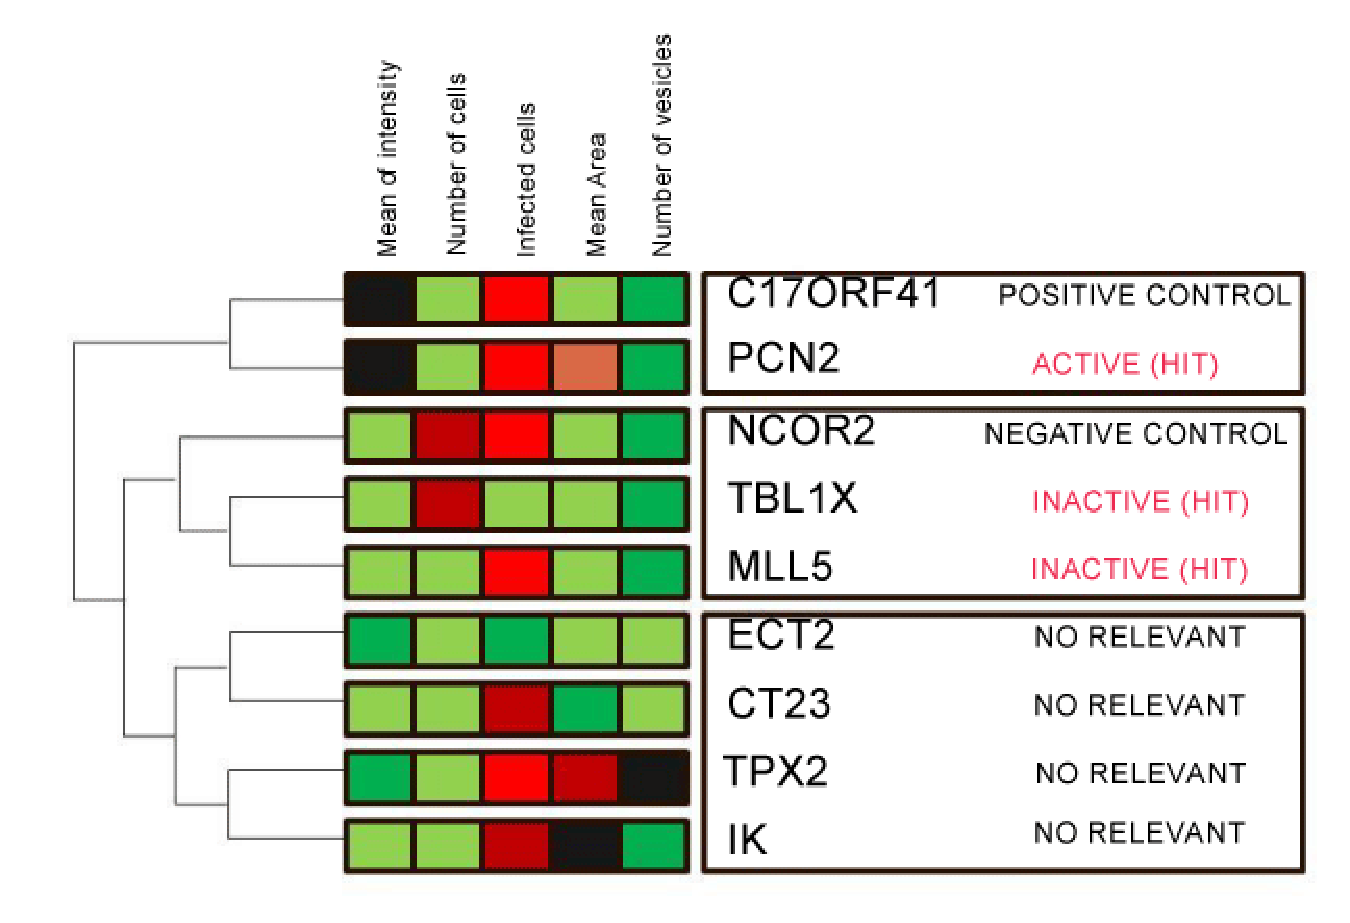
\includegraphics[width=4in] {L5-clustering-closestpair.eps}
%\end{figure}
%
%}
%
%\frame{
%	\frametitle{Practical problem: Nearest neighbor heuristic for TSP}
%
%\begin{figure}
% \includegraphics[width=3in] {L5-TSP-NN.png}
%\end{figure}
%
%}

%\frame{
%	\frametitle{Practical problem: MST heuristic for TSP}
%
%\begin{figure}
% \includegraphics[width=3in] {L5-TSP-MST.png}
%\end{figure}
%
%}


\frame{
\frametitle{{\sc ClosestPair} problem }

\begin{block}{}
 {\bf INPUT: } $n$ points in a plane; \\
 {\bf OUTPUT: } The pair with the least Euclidean distance.
\end{block}

\begin{figure}[H]
\center
	\begin{tikzpicture}[scale=0.9, auto,swap]
\draw[black,fill=gray,opacity=0.5](0,0)rectangle (8,5);
\draw[fill=blue,opacity=0.4](1,1)circle(0.07);

\draw[fill=blue,opacity=0.4](2.1,2)circle(0.07);
\draw[fill=blue,opacity=0.4](2.5,3.2)circle(0.07);
\draw[fill=blue,opacity=0.4](2,1)circle(0.07);
\draw[fill=blue,opacity=0.4](2.8,4.2)circle(0.07);
\draw[fill=blue,opacity=0.4](1.1,4.1)circle(0.07);
\draw[fill=blue,opacity=0.4](1,2)circle(0.07);
\draw[fill=blue,opacity=0.4](1.5,2.4)circle(0.07);
\draw[fill=blue,opacity=0.4](1.3,3.3)circle(0.07);
\draw[fill=blue,opacity=0.4](1,4.6)circle(0.07);
\draw[fill=blue,opacity=0.4](3,3.4)circle(0.07);
\draw[fill=blue,opacity=0.4](3,4)circle(0.07);
\draw[fill=blue,opacity=0.4](4,4.6)circle(0.07);
\draw[fill=blue,opacity=0.4](5,2)circle(0.07);
\draw[fill=blue,opacity=0.4](6,2.3)circle(0.07);
\draw[fill=blue,opacity=0.4](4,1)circle(0.07);
\draw[fill=blue,opacity=0.4](5,3)circle(0.07);
\draw[fill=blue,opacity=0.4](7,4)circle(0.07);
\draw[fill=blue,opacity=0.4](7.5,2)circle(0.07);
\draw[fill=blue,opacity=0.4](7.1,1)circle(0.07);
\draw[fill=blue,opacity=0.4](7.8,0.5)circle(0.07);
\draw[fill=blue,opacity=0.4](7,3)circle(0.07);
\draw[fill=blue,opacity=0.4](7.5,1.5)circle(0.07);
\draw[fill=blue,opacity=0.4](5,2)circle(0.07);
\draw[fill=blue,opacity=0.4](3,1)circle(0.07);
\draw[fill=blue,opacity=0.4](3,0.5)circle(0.07);
\draw[fill=blue,opacity=0.4](5,1.2)circle(0.07);


    \end{tikzpicture}	
%\caption{L5-clustering-closestpair.eps}		
\end{figure}


}

\frame{
\frametitle{About {\sc ClosestPair} problem }
\begin{itemize}
 \item Computational geometry: M. Shamos and D. Hoey were working out efficient algorithm for basic computational primitive in CG in 1970's. They asked a question: does there exist an algorithm using less than $O(n^2)$ time? 
\end{itemize}

\begin{itemize}
 \item 
 1D case:  it is easy to solve the problem in $ O(n \log n)$ via sorting. 
\item 
2D case:  a brute-force algorithm works in  $O(n^2)$ time by checking all possible pairs. 

\item \textcolor{black}{\bf Question:} can we find a faster method?
\end{itemize}


}

\frame{
\begin{block}{}
 Trial 1: Divide into 4 subsets
\end{block}
}


\frame{
\frametitle{Trial 1: {\sc Divide and Conquer} (4 subsets) }
\begin{itemize}
\item 
{\sc Divide and Conquer}: divide into 4 subsets.

\begin{figure}[H]
\center
	\begin{tikzpicture}[scale=0.9, auto,swap]

%???????%??????????????2???
%\fill[xstep=120pt,ystep=60pt,gray]
%(0,0)grid(240pt,120pt);
\draw[black,fill=gray,opacity=0.5](0,0)rectangle (3.2,2.5);
\draw[fill=blue,opacity=0.4](1,1)circle(0.07);
\draw[fill=blue,opacity=0.4](2,2)circle(0.07);
\draw[fill=blue,opacity=0.4](2.1,2.4)circle(0.07);
\draw[fill=blue,opacity=0.4](0.5,1.5)circle(0.07);
\draw[fill=blue,opacity=0.4](0.4,0.4)circle(0.07);
\draw[fill=blue,opacity=0.4](0.1,2.3)circle(0.07);
\draw[fill=blue,opacity=0.4](0.8,2)circle(0.07);
\draw[fill=blue,opacity=0.4](3,2)circle(0.07);
\draw[fill=blue,opacity=0.4](3,0.4)circle(0.07);
\draw[fill=blue,opacity=0.4](3.1,1.3)circle(0.07);
\draw[fill=blue,opacity=0.4](2.5,0.2)circle(0.07);
\draw[fill=blue,opacity=0.4](1.5,0.2)circle(0.07);
\draw[fill=blue,opacity=0.4](1.6,1.5)circle(0.07);
\draw[fill=blue,opacity=0.4](2.8,1.7)circle(0.07);
\draw[fill=blue,opacity=0.4](2,1)circle(0.07);


\draw[black,fill=gray,opacity=0.5](3.2,0)rectangle (8,2.5);

\draw[fill=blue,opacity=0.4](7,2)circle(0.07);

\draw[black,fill=gray,opacity=0.5](0,0)rectangle (3.2,-2.5);

\draw[fill=blue,opacity=0.4](0.5,-2)circle(0.07);
\draw[black,fill=gray,opacity=0.5](3.2,0)rectangle (8,-2.5);
\draw[fill=blue,opacity=0.4](7,-2.1)circle(0.07);
\draw[fill=blue,opacity=0.4](5,-1.2)circle(0.07);
\draw[fill=blue,opacity=0.4](5.6,-0.2)circle(0.07);
\draw[fill=blue,opacity=0.4](5.3,-0.5)circle(0.07);
\draw[fill=blue,opacity=0.4](5.6,-0.9)circle(0.07);
\draw[fill=blue,opacity=0.4](5.2,-2.2)circle(0.07);
\draw[fill=blue,opacity=0.4](6,-1.5)circle(0.07);
\draw[fill=blue,opacity=0.4](3.5,-1.2)circle(0.07);
\draw[fill=blue,opacity=0.4](3.6,-0.2)circle(0.07);
\draw[fill=blue,opacity=0.4](3.7,-1.6)circle(0.07);
\draw[fill=blue,opacity=0.4](4,-2)circle(0.07);
\draw[fill=blue,opacity=0.4](4.3,-0.3)circle(0.07);
\draw[fill=blue,opacity=0.4](4.6,-1.3)circle(0.07);

%\node at (3.8,1.8){L};
    \end{tikzpicture}	
%\caption{L5-closestpair-4subsets.eps}		
\end{figure}

%\begin{figure}
% 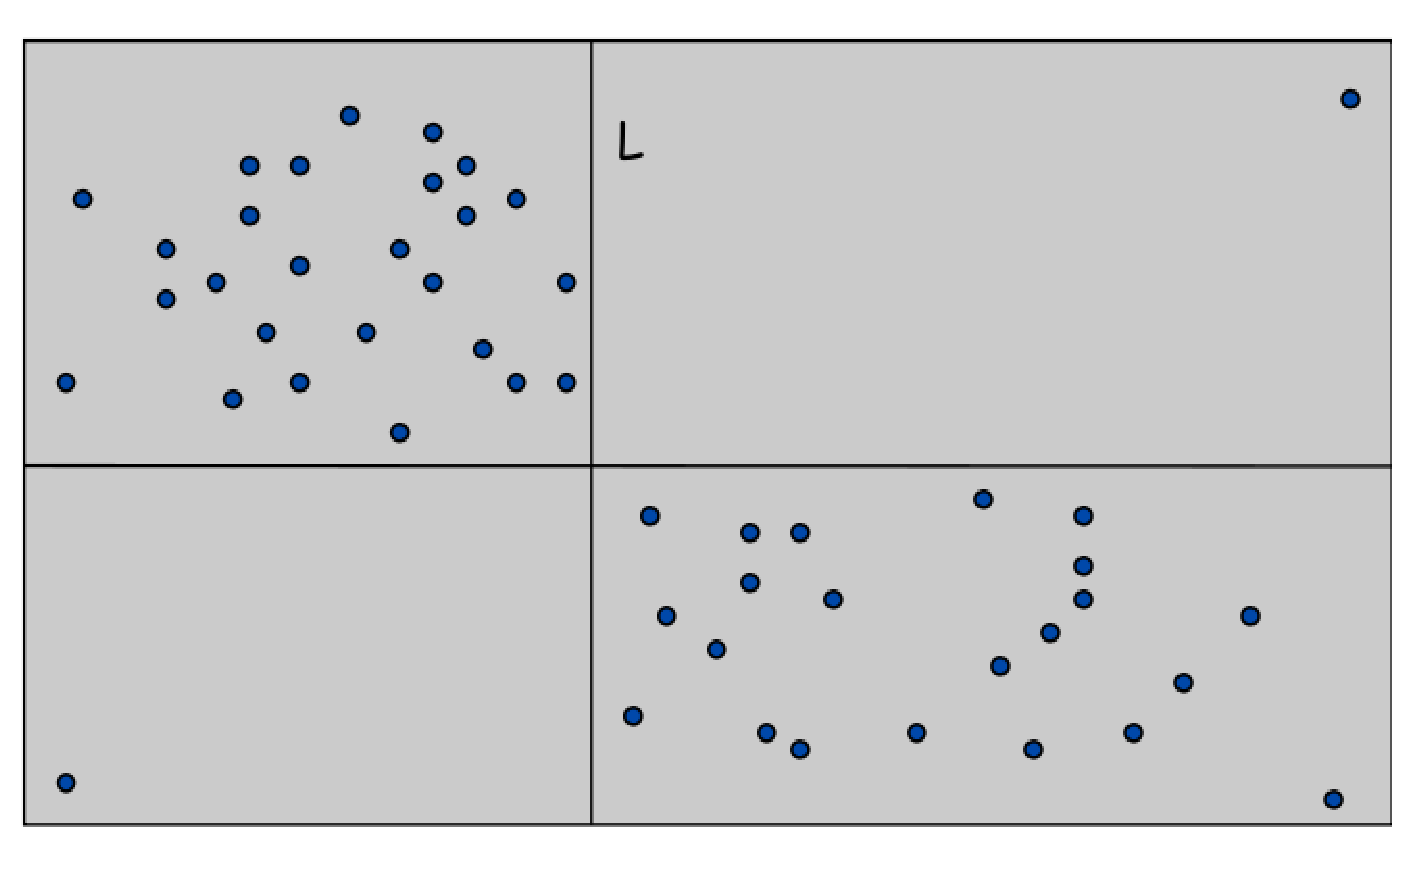
\includegraphics[width=3in] {L5-closestpair-4subsets.eps}
%\end{figure}

\item Difficulties: 
	\begin{itemize}
		\item 
The subsets might be unbalanced  --- we cannot guarantee that each subset has approximately $\frac{n}{4}$ points. 
		\item Since the closest pair might lie in different subsets, we need to consider all ${4}\choose{2}$ pairs of subsets to avoid missing the closest pair, thus complicating  the ``combine" step. 
	\end{itemize}

\end{itemize}

}

\frame{
\begin{block}{}
Trial 2: Divide into 2 halves
\end{block}
}


\frame{
\frametitle{Trial 2: {\sc Divide and Conquer} (2 subsets) }
\begin{itemize}
 \item \textcolor{blue}{\bf Divide:} divide into two halves with equal size.  \\ It is easy to achieve this through sorting by $x$ coordinate first, and then select the median as pivot.
\end{itemize}

\begin{figure}[H]
\center
	\begin{tikzpicture}[scale=0.9, auto,swap]
\draw[black,fill=gray,opacity=0.5](0,0)rectangle (3.2,5);
\draw[black,fill=gray,opacity=0.5](3.2,0)rectangle (8,5);
\draw[fill=blue,opacity=0.4](1,1)circle(0.07);

\draw[fill=blue,opacity=0.4](2.1,2)circle(0.07);
\draw[fill=blue,opacity=0.4](2.5,3.2)circle(0.07);
\draw[fill=blue,opacity=0.4](2,1)circle(0.07);
\draw[fill=blue,opacity=0.4](2.8,4.2)circle(0.07);
\draw[fill=blue,opacity=0.4](1.1,4.1)circle(0.07);
\draw[fill=blue,opacity=0.4](1,2)circle(0.07);
\draw[fill=blue,opacity=0.4](1.5,2.4)circle(0.07);
\draw[fill=blue,opacity=0.4](1.3,3.3)circle(0.07);
\draw[fill=blue,opacity=0.4](1,4.6)circle(0.07);
\draw[fill=blue,opacity=0.4](3,3.4)circle(0.07);
\draw[fill=blue,opacity=0.4](3,4)circle(0.07);
\draw[fill=blue,opacity=0.4](4,4.6)circle(0.07);
\draw[fill=blue,opacity=0.4](5,2)circle(0.07);
\draw[fill=blue,opacity=0.4](6,2.3)circle(0.07);
\draw[fill=blue,opacity=0.4](4,1)circle(0.07);
\draw[fill=blue,opacity=0.4](5,3)circle(0.07);
\draw[fill=blue,opacity=0.4](7,4)circle(0.07);
\draw[fill=blue,opacity=0.4](7.5,2)circle(0.07);
\draw[fill=blue,opacity=0.4](7.1,1)circle(0.07);
\draw[fill=blue,opacity=0.4](7.8,0.5)circle(0.07);
\draw[fill=blue,opacity=0.4](7,3)circle(0.07);
\draw[fill=blue,opacity=0.4](7.5,1.5)circle(0.07);
\draw[fill=blue,opacity=0.4](5,2)circle(0.07);
\draw[fill=blue,opacity=0.4](3,1)circle(0.07);
\draw[fill=blue,opacity=0.4](3,0.5)circle(0.07);
\draw[fill=blue,opacity=0.4](5,1.2)circle(0.07);

    \end{tikzpicture}	
\end{figure}



%\begin{figure}
 %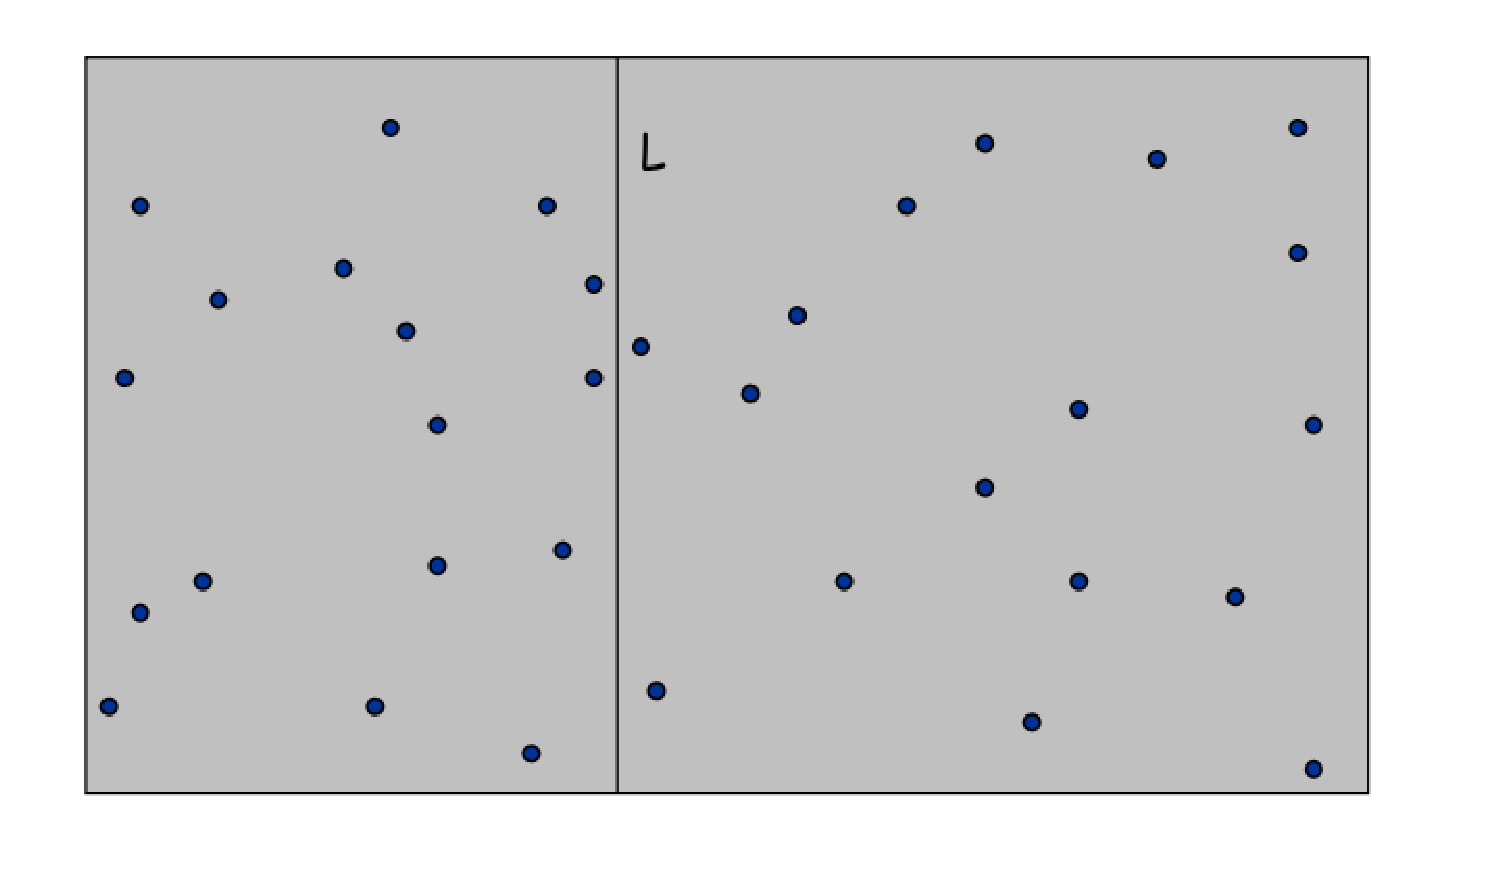
\includegraphics[width=3in]{L5-closestpair.eps}
%\end{figure}

}

\frame{
\frametitle{Trial 2: {\sc Divide and Conquer} (2 subsets) }
\begin{itemize}
 \item  \textcolor{blue}{\bf Divide:}  dividing into two (roughly equal) subsets;
 \item \textcolor{blue}{\bf Conquer:} finding closest pairs in each  half;
\end{itemize}

\begin{figure}[H]
\center
	\begin{tikzpicture}[scale=0.9, auto,swap]
\draw[black,fill=gray,opacity=0.5](0,0)rectangle (3.2,5);
\draw[black,fill=gray,opacity=0.5](3.2,0)rectangle (8,5);
\draw[fill=blue,opacity=0.4](1,1)circle(0.07);

\draw[fill=blue,opacity=0.4](2.1,2)circle(0.07);
\draw[fill=blue,opacity=0.4](2.5,3.2)circle(0.07);
\draw[fill=blue,opacity=0.4](2,1)circle(0.07);
\draw[fill=blue,opacity=0.4](2.8,4.2)circle(0.07);
\draw[fill=blue,opacity=0.4](1.1,4.1)circle(0.07);
\draw[fill=red,opacity=0.4](1,2)circle(0.07);
\draw[fill=red,opacity=0.4](1.5,2.4)circle(0.07);
\draw[fill=blue,opacity=0.4](1.3,3.3)circle(0.07);
\draw[fill=blue,opacity=0.4](1,4.6)circle(0.07);
\draw[fill=blue,opacity=0.4](3,3.4)circle(0.07);
\draw[fill=blue,opacity=0.4](3,4)circle(0.07);
\draw[fill=blue,opacity=0.4](4,4.6)circle(0.07);
\draw[fill=blue,opacity=0.4](5,2)circle(0.07);
\draw[fill=blue,opacity=0.4](6,2.3)circle(0.07);
\draw[fill=blue,opacity=0.4](4,1)circle(0.07);
\draw[fill=blue,opacity=0.4](5,3)circle(0.07);
\draw[fill=blue,opacity=0.4](7,4)circle(0.07);
\draw[fill=blue,opacity=0.4](7.5,2)circle(0.07);
\draw[fill=blue,opacity=0.4](7.1,1)circle(0.07);
\draw[fill=blue,opacity=0.4](7.8,0.5)circle(0.07);
\draw[fill=blue,opacity=0.4](7,3)circle(0.07);
\draw[fill=blue,opacity=0.4](7.5,1.5)circle(0.07);
\draw[fill=blue,opacity=0.4](5,2)circle(0.07);
\draw[fill=blue,opacity=0.4](3,1)circle(0.07);
\draw[fill=blue,opacity=0.4](3,0.5)circle(0.07);
\draw[fill=blue,opacity=0.4](5,1.2)circle(0.07);

\draw[black,fill=red,opacity=0.4](1,2)circle(0.07);
\draw[black,fill=red,opacity=0.4](1.5,2.4)circle(0.07);
\draw [red](1+0.07,2+0.07)-- (1.5-0.07,2.4-0.07);
\node at (1.1,2.5){21};

\draw[black,fill=red,opacity=0.4](4.3,3)circle(0.07);
\draw[black,fill=red,opacity=0.4](4.8,3.7)circle(0.07);
\draw [red](4.3+0.07,3+0.07)-- (4.8-0.07,3.7-0.07);
\node at (4.3,3.5){12};

    \end{tikzpicture}	
\end{figure}

}

\frame{
\frametitle{Trial 2: {\sc Divide and Conquer} (2 subsets)}
\begin{itemize}
\item \textcolor{blue}{\bf Combine: } It suffices to consider the pairs consisting of one  point from left half and one  point from right half.  Simply examining all such pairs will take $O(n^2)$ time.
\end{itemize}

\begin{figure}[H]
\center
	\begin{tikzpicture}[scale=0.9, auto,swap]
\draw[black,fill=gray,opacity=0.5](0,0)rectangle (3.2,5);
\draw[black,fill=gray,opacity=0.5](3.2,0)rectangle (8,5);
\draw[fill=blue,opacity=0.4](1,1)circle(0.07);

\draw[fill=blue,opacity=0.4](2.1,2)circle(0.07);
\draw[fill=blue,opacity=0.4](2.5,3.2)circle(0.07);
\draw[fill=blue,opacity=0.4](2,1)circle(0.07);
\draw[fill=blue,opacity=0.4](2.8,4.2)circle(0.07);
\draw[fill=blue,opacity=0.4](1.1,4.1)circle(0.07);
\draw[fill=blue,opacity=0.4](1.3,3.3)circle(0.07);
\draw[fill=blue,opacity=0.4](1,4.6)circle(0.07);
\draw[fill=blue,opacity=0.4](3,3.4)circle(0.07);
\draw[fill=blue,opacity=0.4](3,4)circle(0.07);
\draw[fill=blue,opacity=0.4](4,4.6)circle(0.07);
\draw[fill=blue,opacity=0.4](5,2)circle(0.07);
\draw[fill=blue,opacity=0.4](6,2.3)circle(0.07);
\draw[fill=blue,opacity=0.4](4,1)circle(0.07);
\draw[fill=blue,opacity=0.4](5,3)circle(0.07);
\draw[fill=blue,opacity=0.4](7,4)circle(0.07);
\draw[fill=blue,opacity=0.4](7.5,2)circle(0.07);
\draw[fill=blue,opacity=0.4](7.1,1)circle(0.07);
\draw[fill=blue,opacity=0.4](7.8,0.5)circle(0.07);
\draw[fill=blue,opacity=0.4](7,3)circle(0.07);
\draw[fill=blue,opacity=0.4](7.5,1.5)circle(0.07);
\draw[fill=blue,opacity=0.4](5,2)circle(0.07);
\draw[fill=blue,opacity=0.4](3,1)circle(0.07);
\draw[fill=blue,opacity=0.4](3,0.5)circle(0.07);
\draw[fill=blue,opacity=0.4](5,1.2)circle(0.07);

\draw[black,fill=red,opacity=0.4](1,2)circle(0.07);
\draw[black,fill=red,opacity=0.4](1.5,2.4)circle(0.07);
\draw [red](1+0.07,2+0.07)-- (1.5-0.07,2.4-0.07);
\node at (1.1,2.5){21};

\draw[black,fill=red,opacity=0.4](4.3,3)circle(0.07);
\draw[black,fill=red,opacity=0.4](4.8,3.7)circle(0.07);
\draw [red](4.3+0.07,3+0.07)-- (4.8-0.07,3.7-0.07);
\node at (4.3,3.5){12};

\draw[black,fill=red,opacity=0.4](3,2.1)circle(0.07);
\draw[black,fill=red,opacity=0.4](3.3,2.3)circle(0.07);
\draw [red](3+0.07,2.1+0.07)-- (3.3-0.07,2.3-0.07);
\node at (3,2.4){8};

    \end{tikzpicture}	
\end{figure}

}

\frame{
	\frametitle{Two types of redundancy} 
\begin{figure}[H]
\center
	\begin{tikzpicture}[scale=0.9, auto,swap]
\draw[black,fill=gray,opacity=0.5](0,0)rectangle (3.2,5);
\draw[black,fill=gray,opacity=0.5](3.2,0)rectangle (8,5);
\draw[fill=blue,opacity=0.4](1,1)circle(0.07);

\draw[fill=blue,opacity=0.4](2.1,2)circle(0.07);
\draw[fill=blue,opacity=0.4](2.5,3.2)circle(0.07);
\draw[fill=blue,opacity=0.4](2,1)circle(0.07);
\draw[fill=blue,opacity=0.4](2.8,4.2)circle(0.07);
\draw[fill=blue,opacity=0.4](1.1,4.1)circle(0.07);
\draw[fill=blue,opacity=0.4](1.3,3.3)circle(0.07);
\draw[fill=blue,opacity=0.4](1,4.6)circle(0.07);
\draw[fill=blue,opacity=0.4](3,3.4)circle(0.07);
\draw[fill=blue,opacity=0.4](3,4)circle(0.07);
\draw[fill=blue,opacity=0.4](4,4.6)circle(0.07);
\draw[fill=blue,opacity=0.4](5,2)circle(0.07);
\draw[fill=blue,opacity=0.4](6,2.3)circle(0.07);
\draw[fill=blue,opacity=0.4](4,1)circle(0.07);
\draw[fill=blue,opacity=0.4](5,3)circle(0.07);
\draw[fill=blue,opacity=0.4](7,4)circle(0.07);
\draw[fill=blue,opacity=0.4](7.5,2)circle(0.07);
\draw[fill=blue,opacity=0.4](7.1,1)circle(0.07);
\draw[fill=blue,opacity=0.4](7.8,0.5)circle(0.07);
\draw[fill=blue,opacity=0.4](7,3)circle(0.07);
\draw[fill=blue,opacity=0.4](7.5,1.5)circle(0.07);
\draw[fill=blue,opacity=0.4](5,2)circle(0.07);
\draw[fill=blue,opacity=0.4](3,1)circle(0.07);
\draw[fill=blue,opacity=0.4](3,0.5)circle(0.07);
\draw[fill=blue,opacity=0.4](5,1.2)circle(0.07);

\draw[black,fill=red,opacity=0.4](1,2)circle(0.07);
\draw[black,fill=red,opacity=0.4](1.5,2.4)circle(0.07);
\draw [red](1+0.07,2+0.07)-- (1.5-0.07,2.4-0.07);
\node at (1.1,2.5){21};

\draw[black,fill=red,opacity=0.4](4.3,3)circle(0.07);
\draw[black,fill=red,opacity=0.4](4.8,3.7)circle(0.07);
\draw [red](4.3+0.07,3+0.07)-- (4.8-0.07,3.7-0.07);
\node at (4.3,3.5){12};

\draw[black,fill=red,opacity=0.4](3,2.1)circle(0.07);
\draw[black,fill=red,opacity=0.4](3.3,2.3)circle(0.07);
\draw [red](3+0.07,2.1+0.07)-- (3.3-0.07,2.3-0.07);
\node at (3,2.4){8};

    \end{tikzpicture}	
\end{figure}
\begin{itemize}
	\item It is redundant to calculate distance between $p_i$ and $p_j$ if
		\begin{itemize}
			\item $| x_i - x_j | \geq 12$, or 
			\item $|y_j - y_j | \geq 12 $
		\end{itemize}

\end{itemize}

}
%	\item Can we accomplish the \textcolor{blue}{\bf combine} step in $O(n)$ time? 

\frame{
\frametitle{Remove redundancy of type 1    } 
\begin{itemize}
\item 
\textcolor{blue}{\bf Observation 1:}  
\begin{itemize}
\item The third type occurs in \textcolor{red}{\bf a narrow strip} only; thus, it suffices to check point pairs within the $2\delta$-strip. 
\item Here, $\delta$ is the minimum of {\sc ClosestPair(LeftHalf)} and {\sc ClosestPair(RightHalf)}.\\
\end{itemize}
\end{itemize}

\begin{figure}[H]
\center
	\begin{tikzpicture}[scale=0.9, auto,swap]
\draw[black,fill=gray,opacity=0.5](0,0) rectangle (2.5,5);
\draw[black,fill=black,opacity=0.5](2.5,0) rectangle (3.1,5);
\draw[black,fill=black,opacity=0.5](3.1,0) rectangle (3.7,5);
\draw[black,fill=gray,opacity=0.5](3.7,0) rectangle (8,5);
%??????V?OE??????????????(C)?oe??
\draw[black,fill=black,opacity=0.5](6.2,1.5) rectangle (9.4,2);
 \node  [white,scale=0.85,thick] at(7.8,1.7) {$\delta=\min(12,21)$};

%??????????(R)-????\delta???
\draw[<->,thick,>=stealth,black,fill=black,opacity=0.5](3.1,-0.2) -- (3.7,-0.2);
\node [scale=0.85]at(3.9,-0.2){$\delta$};

\draw[fill=blue,opacity=0.4](1,1)circle(0.07);

\draw[fill=blue,opacity=0.4](2.1,2)circle(0.07);
\draw[fill=blue,opacity=0.4](2.5,3.2)circle(0.07);
\draw[fill=blue,opacity=0.4](2,1)circle(0.07);
\draw[fill=blue,opacity=0.4](2.8,4.2)circle(0.07);
\draw[fill=blue,opacity=0.4](1.1,4.1)circle(0.07);
\draw[fill=blue,opacity=0.4](1.3,3.3)circle(0.07);
\draw[fill=blue,opacity=0.4](1,4.6)circle(0.07);
\draw[fill=blue,opacity=0.4](3,3.4)circle(0.07);
\draw[fill=blue,opacity=0.4](3,4)circle(0.07);
\draw[fill=blue,opacity=0.4](4,4.6)circle(0.07);
\draw[fill=blue,opacity=0.4](5,2)circle(0.07);
\draw[fill=blue,opacity=0.4](6,2.3)circle(0.07);
\draw[fill=blue,opacity=0.4](4,1)circle(0.07);
\draw[fill=blue,opacity=0.4](5,3)circle(0.07);
\draw[fill=blue,opacity=0.4](7,4)circle(0.07);
\draw[fill=blue,opacity=0.4](7.5,4)circle(0.07);
\draw[fill=blue,opacity=0.4](7.1,1)circle(0.07);
\draw[fill=blue,opacity=0.4](7.8,0.5)circle(0.07);
\draw[fill=blue,opacity=0.4](7,3)circle(0.07);
\draw[fill=blue,opacity=0.4](7.5,3.5)circle(0.07);
\draw[fill=blue,opacity=0.4](5,2)circle(0.07);
\draw[fill=blue,opacity=0.4](3,1)circle(0.07);
\draw[fill=blue,opacity=0.4](3,0.5)circle(0.07);
\draw[fill=blue,opacity=0.4](5,1.2)circle(0.07);

\draw[black,fill=red,opacity=0.4](1,2)circle(0.07);
\draw[black,fill=red,opacity=0.4](1.5,2.4)circle(0.07);
\draw[black,fill=red,opacity=0.4](1,2)circle(0.07);
\draw[black,fill=red,opacity=0.4](1.5,2.4)circle(0.07);
\draw [red](1+0.07,2+0.07)-- (1.5-0.07,2.4-0.07);
\node at (1.1,2.5){21};

\draw[black,fill=red,opacity=0.4](4.3,3)circle(0.07);
\draw[black,fill=red,opacity=0.4](4.8,3.7)circle(0.07);

\draw[black,fill=red,opacity=0.4](4.3,3)circle(0.07);
\draw[black,fill=red,opacity=0.4](4.8,3.7)circle(0.07);
\draw [red](4.3+0.07,3+0.07)-- (4.8-0.07,3.7-0.07);
\node at (4.3,3.5){12};

\draw[fill=blue,opacity=0.4](3.3,3)circle(0.07);
\draw[fill=blue,opacity=0.4](3.4,1)circle(0.07);

    \end{tikzpicture}	
\end{figure}

} 

\frame{
\frametitle{Remove redundancy of type 2    } 
\begin{itemize}
\item 
\textcolor{blue}{\bf Observation 2:}  
\begin{itemize}
\item 
Moreover, it is unnecessary to explore \textcolor{red}{\bf all} point pairs within the $2\delta$-strip. In fact, for each point $p_i$, it suffices to examine 11 points for possible closest partners. 
\item 
Let's divide the $2\delta$-strip into grids (size: $\frac{\delta}{2} \times \frac{\delta}{2} $). A grid contains \textcolor{red}{\bf at most one}  point.  
\item 
If  two points are 2 rows apart,  the distance between them should be over  $\delta$ and thus cannot form closest pair. 
\item Example:  For point $27$, it suffices to search within 2 rows for possible closest partners ($<\delta$). 
\end{itemize}
\end{itemize}

\begin{figure}[H]
\center
	\begin{tikzpicture}[scale=0.9, auto,swap]
\draw[black,fill=gray,opacity=0.5](0,0) rectangle (1.2,1.8);
\draw[black,fill=gray,opacity=0.5](1.2,0) rectangle (2.4,1.8);
\draw[black,fill=red,opacity=0.5,step=0.6](0,-1.8)grid(1.2,0);
\draw[black,fill=gray,opacity=0.5,step=0.6](1.2,-1.8)grid(2.4,0);
\draw[black,fill=gray,opacity=0.5](0,-2.8) rectangle (1.2,-1.8);
\draw[black,fill=gray,opacity=0.5](1.2,-2.8) rectangle (2.4,-1.8);

%draw node #1
\draw[fill=blue!70](0.4,0.7)circle(0.15);
\node [white,scale=0.65]at (0.4,0.7){31};
\draw[fill=black](0.6,1.2)circle(0.05);
\draw[fill=black](0.75,1.2)circle(0.05);
\draw[fill=black](0.9,1.2)circle(0.05);
%draw node #2
\draw[fill=blue!70](1.5,1)circle(0.15);
\node [white,scale=0.65]at (1.5,1){39};
\draw [<-](1.9,1)--(2.1,1);
\node[scale=0.85] at (2.2,1) {$j$};
%draw node #3
\draw[fill=blue!70](0.4,-1)circle(0.15);
\node [white,scale=0.65]at (0.4,-1){29};

\draw[fill=blue!70](1.6,-0.8)circle(0.15);
\node [white,scale=0.65]at (1.6,-0.8){30};

\draw[fill=blue!70](0.3,-1.6)circle(0.15);
\node [white,scale=0.65]at (0.3,-1.6){27};

\draw[fill=blue!70](2,-1.5)circle(0.15);
\node [white,scale=0.65]at (2,-1.5){28};

\draw[fill=blue!70](0.6,-2.7)circle(0.15);
\node [white,scale=0.65]at (0.6,-2.7){26};

%1/2 deta
\node[scale=0.85] at (2.8,-0.3) {$\frac{1}{2}\delta$};
\node[scale=0.85] at (2.8,-0.9) {$\frac{1}{2}\delta$};
\node[scale=0.85] at (2.8,-1.5) {$\frac{1}{2}\delta$};
    \end{tikzpicture}	
\end{figure}



}

\frame{
\frametitle{To detect potential closest pair: Case 1}

\begin{figure}[H]
\center
	\begin{tikzpicture}[scale=0.9, auto,swap]
\draw[black,fill=gray,opacity=0.5](0,0) rectangle (1.2,1.8);
\draw[black,fill=gray,opacity=0.5](1.2,0) rectangle (2.4,1.8);
\draw[black,fill=red,opacity=0.5,step=0.6](0,-1.8)grid(1.2,0);
\draw[black,fill=gray,opacity=0.5,step=0.6](1.2,-1.8)grid(2.4,0);
\draw[black,fill=gray,opacity=0.5](0,-2.8) rectangle (1.2,-1.8);
\draw[black,fill=gray,opacity=0.5](1.2,-2.8) rectangle (2.4,-1.8);

%draw node #1
\draw[fill=blue!70](0.4,0.7)circle(0.15);
\node [white,scale=0.65]at (0.4,0.7){31};
\draw[fill=black,opacity=0.4](0.6,1.2)circle(0.05);
\draw[fill=black,opacity=0.4](0.75,1.2)circle(0.05);
\draw[fill=black,opacity=0.4](0.9,1.2)circle(0.05);
%draw node #2
\draw[fill=blue!70](1.5,1)circle(0.15);
\node [white,scale=0.65]at (1.5,1){39};
\draw [<-](1.9,1)--(2.1,1);
\node[scale=0.85] at (2.2,1) {$j$};
%draw node #3
\draw[fill=blue!70](0.4,-1)circle(0.15);
%\node [white,scale=0.65]at (0.4,-1){29};
%#add
\draw[fill=blue!70](0.4,-0.4)circle(0.15);
\draw[fill=blue!70](0.9,-0.4)circle(0.15);
\draw[fill=blue!70](0.9,-1)circle(0.15);
\draw[fill=blue!70](0.9,-1.4)circle(0.15);
%#add
\draw[fill=red!70](1.6,-0.8)circle(0.15);
%\node [white,scale=0.65]at (1.6,-0.8){30};
\draw[fill=red!70](1.6,-0.3)circle(0.15);
\draw[fill=red!70](1.6,-1.5)circle(0.15);
\draw[fill=blue!70](2.1,-0.3)circle(0.15);
\draw[fill=blue!70](2.1,-0.9)circle(0.15);

\draw[fill=green!70](0.3,-1.6)circle(0.15);
%\node [white,scale=0.65]at (0.3,-1.6){27};

\draw[fill=blue!70](2,-1.5)circle(0.15);
%\node [white,scale=0.65]at (2,-1.5){28};

\draw[fill=blue!70](0.6,-2.7)circle(0.15);
%\node [white,scale=0.65]at (0.6,-2.7){26};

%1/2 deta
\node[scale=0.85] at (2.8,-0.3) {$\frac{1}{2}\delta$};
\node[scale=0.85] at (2.8,-0.9) {$\frac{1}{2}\delta$};
\node[scale=0.85] at (2.8,-1.5) {$\frac{1}{2}\delta$};
    \end{tikzpicture}	
\end{figure}


\begin{itemize}
 \item Green: point $i$;
 \item  Red: the possible closest partner (distance $<\delta$) of point $i$;
 \end{itemize}
}

\frame{
\frametitle{To detect potential closest pair: Case 2}

%\begin{figure}
% \includegraphics[width=3in] {L5-closestpair-1221delta-strip-7-reason2.eps}
%\end{figure}

\begin{figure}[H]
\center
	\begin{tikzpicture}[scale=0.9, auto,swap]
\draw[black,fill=gray,opacity=0.5](0,0) rectangle (1.2,1.8);
\draw[black,fill=gray,opacity=0.5](1.2,0) rectangle (2.4,1.8);
\draw[black,fill=red,opacity=0.5,step=0.6](0,-1.8)grid(1.2,0);
\draw[black,fill=gray,opacity=0.5,step=0.6](1.2,-1.8)grid(2.4,0);
\draw[black,fill=gray,opacity=0.5](0,-2.8) rectangle (1.2,-1.8);
\draw[black,fill=gray,opacity=0.5](1.2,-2.8) rectangle (2.4,-1.8);

%draw node #1
\draw[fill=blue!70](0.4,0.7)circle(0.15);
\node [white,scale=0.65]at (0.4,0.7){31};
\draw[fill=black,opacity=0.4](0.6,1.2)circle(0.05);
\draw[fill=black,opacity=0.4](0.75,1.2)circle(0.05);
\draw[fill=black,opacity=0.4](0.9,1.2)circle(0.05);
%draw node #2
\draw[fill=blue!70](1.5,1)circle(0.15);
\node [white,scale=0.65]at (1.5,1){39};
\draw [<-](1.9,1)--(2.1,1);
\node[scale=0.85] at (2.2,1) {$j$};
%draw node #3
\draw[fill=blue!70](0.4,-1)circle(0.15);
%\node [white,scale=0.65]at (0.4,-1){29};
%#add
\draw[fill=blue!70](0.4,-0.4)circle(0.15);
\draw[fill=blue!70](0.9,-0.4)circle(0.15);
\draw[fill=blue!70](0.9,-1)circle(0.15);
\draw[fill=green!70](0.9,-1.4)circle(0.15);
%#add
\draw[fill=red!70](1.6,-0.8)circle(0.15);
%\node [white,scale=0.65]at (1.6,-0.8){30};
\draw[fill=red!70](1.6,-0.3)circle(0.15);
\draw[fill=red!70](1.6,-1.5)circle(0.15);
\draw[fill=red!70](2.1,-0.3)circle(0.15);
\draw[fill=red!70](2.1,-0.9)circle(0.15);

\draw[fill=blue!70](0.3,-1.6)circle(0.15);
%\node [white,scale=0.65]at (0.3,-1.6){27};

\draw[fill=red!70](2,-1.5)circle(0.15);
%\node [white,scale=0.65]at (2,-1.5){28};

\draw[fill=blue!70](0.6,-2.7)circle(0.15);
%\node [white,scale=0.65]at (0.6,-2.7){26};

%1/2 deta
\node[scale=0.85] at (2.8,-0.3) {$\frac{1}{2}\delta$};
\node[scale=0.85] at (2.8,-0.9) {$\frac{1}{2}\delta$};
\node[scale=0.85] at (2.8,-1.5) {$\frac{1}{2}\delta$};
    \end{tikzpicture}	
\end{figure}


\begin{itemize}
 \item Green: point $i$;
 \item  Red: the possible closest partner (distance  $<\delta$) of point $i$;
\end{itemize}
}

%\frame{
%\frametitle{To detect potential closest pair: Case 3}
%
%\begin{figure}
% \includegraphics[width=3in] {L5-closestpair-1221delta-strip-7-reason3.eps}
%\end{figure}
%\begin{itemize}
% \item Green: point $i$;
% \item  Red: the possible closest partner (distance  $<\delta$) of point $i$;
%\end{itemize}
%}

%\frame{
%\frametitle{Detect potential closest pair}
%
%\begin{figure}[H]
%\center
%	\begin{tikzpicture}[scale=0.9, auto,swap]
%\draw[black,fill=gray,opacity=0.4](0,0) rectangle (1.2,1.8);
%\draw[black,fill=gray,opacity=0.4](1.2,0) rectangle (2.4,1.8);
%\draw[black,fill=red,opacity=0.4,step=0.6](0,-1.8)grid(1.2,0);
%\draw[black,fill=gray,opacity=0.4,step=0.6](1.2,-1.8)grid(2.4,0);
%\draw[black,fill=gray,opacity=0.4](0,-2.8) rectangle (1.2,-1.8);
%\draw[black,fill=gray,opacity=0.4](1.2,-2.8) rectangle (2.4,-1.8);
%
%%draw node #1
%\draw[fill=blue!70](0.4,0.7)circle(0.15);
%\node [white,scale=0.65]at (0.4,0.7){31};
%\draw[fill=black,opacity=0.4](0.6,1.2)circle(0.05);
%\draw[fill=black,opacity=0.4](0.75,1.2)circle(0.05);
%\draw[fill=black,opacity=0.4](0.9,1.2)circle(0.05);
%%draw node #2
%\draw[fill=blue!70](1.5,1)circle(0.15);
%\node [white,scale=0.65]at (1.5,1){39};
%\draw [<-](1.9,1)--(2.1,1);
%\node[scale=0.85] at (2.2,1) {$j$};
%%draw node #3
%\draw[fill=blue!70](0.4,-1)circle(0.15);
%%\node [white,scale=0.65]at (0.4,-1){29};
%%#add
%\draw[fill=blue!70](0.4,-0.4)circle(0.15);
%\draw[fill=blue!70](0.9,-0.4)circle(0.15);
%\draw[fill=blue!70](0.9,-1)circle(0.15);
%\draw[fill=blue!70](0.9,-1.4)circle(0.15);
%%#add
%\draw[fill=red!70](1.6,-0.8)circle(0.15);
%%\node [white,scale=0.65]at (1.6,-0.8){30};
%\draw[fill=red!70](1.6,-0.3)circle(0.15);
%\draw[fill=red!70](1.6,-1.5)circle(0.15);
%\draw[fill=blue!70](2.1,-0.3)circle(0.15);
%\draw[fill=blue!70](2.1,-0.9)circle(0.15);
%
%\draw[fill=green!70](0.3,-1.6)circle(0.15);
%%\node [white,scale=0.65]at (0.3,-1.6){27};
%
%\draw[fill=blue!70](2,-1.5)circle(0.15);
%%\node [white,scale=0.65]at (2,-1.5){28};
%
%\draw[fill=blue!70](0.6,-2.7)circle(0.15);
%%\node [white,scale=0.65]at (0.6,-2.7){26};
%
%%1/2 deta
%\node[scale=0.85] at (2.8,-0.3) {$\frac{1}{2}\delta$};
%\node[scale=0.85] at (2.8,-0.9) {$\frac{1}{2}\delta$};
%\node[scale=0.85] at (2.8,-1.5) {$\frac{1}{2}\delta$};
%
%
%%??3???????????OE?????OE?
%\draw[fill=blue!70](6,1.8)circle(0.15);
%\draw[fill=red!70](6,1.4)circle(0.15);
%\draw[fill=blue!70](6,1)circle(0.15);
%\draw[fill=blue!70](6,0.6)circle(0.15);
%\draw[fill=blue!70](6,0.2)circle(0.15);
%\draw[fill=red!70](6,-0.2)circle(0.15);
%\draw[fill=blue!70](6,-0.6)circle(0.15);
%\draw[fill=blue!70](6,-1)circle(0.15);
%\draw[fill=blue!70](6,-1.4)circle(0.15);
%\draw[fill=red!70](6,-1.8)circle(0.15);
%\draw[fill=blue!70](6,-2.2)circle(0.15);
%\draw[fill=green!70](6,-2.6)circle(0.15);
%    \end{tikzpicture}	
%\end{figure}
%
%
%
%\begin{itemize}
% \item Green: point $i$;
% \item Red: the possible closest partner ($<\delta$) of point $i$;
%\end{itemize}
%}


\frame{
\frametitle{To detect potential closest pair}

\begin{figure}[H]
\center
	\begin{tikzpicture}[scale=0.9, auto,swap]
\draw[black,fill=gray,opacity=0.4](0,0) rectangle (1.2,1.8);
\draw[black,fill=gray,opacity=0.4](1.2,0) rectangle (2.4,1.8);
\draw[black,fill=red,opacity=0.4,step=0.6](0,-1.8)grid(1.2,0);
\draw[black,fill=gray,opacity=0.4,step=0.6](1.2,-1.8)grid(2.4,0);
\draw[black,fill=gray,opacity=0.4](0,-2.8) rectangle (1.2,-1.8);
\draw[black,fill=gray,opacity=0.4](1.2,-2.8) rectangle (2.4,-1.8);

%draw node #1
\draw[fill=blue!70](0.4,0.7)circle(0.15);
\node [white,scale=0.65]at (0.4,0.7){31};
\draw[fill=black,opacity=0.4](0.6,1.2)circle(0.05);
\draw[fill=black,opacity=0.4](0.75,1.2)circle(0.05);
\draw[fill=black,opacity=0.4](0.9,1.2)circle(0.05);
%draw node #2
\draw[fill=blue!70](1.5,1)circle(0.15);
\node [white,scale=0.65]at (1.5,1){39};
\draw [<-](1.9,1)--(2.1,1);
\node[scale=0.85] at (2.2,1) {$j$};
%draw node #3
\draw[fill=blue!70](0.4,-1)circle(0.15);
%\node [white,scale=0.65]at (0.4,-1){29};
%#add
\draw[fill=blue!70](0.4,-0.4)circle(0.15);
\draw[fill=blue!70](0.9,-0.4)circle(0.15);
\draw[fill=blue!70](0.9,-1)circle(0.15);
\draw[fill=blue!70](0.9,-1.4)circle(0.15);
%#add
\draw[fill=red!70](1.6,-0.8)circle(0.15);
%\node [white,scale=0.65]at (1.6,-0.8){30};
\draw[fill=red!70](1.6,-0.3)circle(0.15);
\draw[fill=red!70](1.6,-1.5)circle(0.15);
\draw[fill=blue!70](2.1,-0.3)circle(0.15);
\draw[fill=blue!70](2.1,-0.9)circle(0.15);

\draw[fill=green!70](0.3,-1.6)circle(0.15);
%\node [white,scale=0.65]at (0.3,-1.6){27};

\draw[fill=blue!70](2,-1.5)circle(0.15);
%\node [white,scale=0.65]at (2,-1.5){28};

\draw[fill=blue!70](0.6,-2.7)circle(0.15);
%\node [white,scale=0.65]at (0.6,-2.7){26};

%1/2 deta
\node[scale=0.85] at (2.8,-0.3) {$\frac{1}{2}\delta$};
\node[scale=0.85] at (2.8,-0.9) {$\frac{1}{2}\delta$};
\node[scale=0.85] at (2.8,-1.5) {$\frac{1}{2}\delta$};


%??3???????????OE?????OE?
\draw[fill=blue!70](6,1.8)circle(0.15);
\draw[fill=red!70](6,1.4)circle(0.15);
\draw[fill=blue!70](6,1)circle(0.15);
\draw[fill=blue!70](6,0.6)circle(0.15);
\draw[fill=blue!70](6,0.2)circle(0.15);
\draw[fill=red!70](6,-0.2)circle(0.15);
\draw[fill=blue!70](6,-0.6)circle(0.15);
\draw[fill=blue!70](6,-1)circle(0.15);
\draw[fill=blue!70](6,-1.4)circle(0.15);
\draw[fill=red!70](6,-1.8)circle(0.15);
\draw[fill=blue!70](6,-2.2)circle(0.15);
\draw[fill=green!70](6,-2.6)circle(0.15);
    \end{tikzpicture}	
\end{figure}



\begin{itemize}
 \item If all points within the strip were sorted by $y$-coordinates, it suffices to  calculate distance between each point with its next 11 neighbors.
 \item Why 11 points here? All red points fall into the subsequent 11 points. 
 %\item Reason:  All the points in red are within 3 rows, which have at most 12 points.
 \end{itemize}
}


\frame{
\frametitle{{\sc ClosestPair} algorithm }
\begin{small}
{\sc ClosestPair}$( p_l, ..., p_r)$
\begin{algorithmic}[1]
\STATE{//To find the closest points within $( p_l, ..., p_r)$. Here we assume that $p_l,...,p_r$ have already been sorted according to $x$-coordinate; }
\IF{$r-l==1$ }
	\RETURN{$d(p_{l}, p_{r})$};
\ENDIF
\STATE Use the $x$-coordinate of $p_{\lfloor\frac{l+r}{2}\rfloor}$ to divide $p_l,...,p_r$ into two halves;  %//\textcolor{red}{$O(n)$}
\STATE $\delta_1$ = {\sc ClosestPair(LeftHalf)};    //\textcolor{red}{$T(\frac{n}{2})$ } 
\STATE $\delta_2$ = {\sc ClosestPair(RightHalf)};   //\textcolor{red}{$T(\frac{n}{2})$ } 
\STATE $\delta = \min( \delta_1, \delta_2);$
\STATE Sort points within the $2\delta$ wide strip  by $y$-coordinate; //\textcolor{red}{$O(n \log n )$ } 
\STATE Scan points in $y$-order and calculate distance between each point with its next 11 neighbors. Update $\delta$ if finding a distance less than $\delta$;  //\textcolor{red}{$O(n)$}
\end{algorithmic}
\end{small}
\begin{itemize}
\item 
Find closest pair within $p_{0}, p_{1}, ..., p_{n-1}$: {\sc ClosestPair}$( p_0, ..., p_{n-1})$
\item Time-complexity: $T(n)=2T(\tfrac{n}{2}) + O(n \log n) = O(n\log^2 n)$.
\end{itemize}

}

\frame{
\frametitle{{\sc ClosestPair} algorithm: improvement }
\begin{itemize}
\item 
Note that if the points within the $2\delta$-wide strip have no structure, we have to sort them from the scratch, which will take $O(n\log n)$ time. 
\item Let's try to introduce some structure into the points within the $2\delta$-wide: If the point within each $\delta$-wide strip were already sorted, it is relatively easy to sort the points within the $2\delta$-wide strip. Specifically,  
\begin{itemize}
 \item Each recursion keeps two sorted list: one list by $x$, and the other list by $y$. 
 \item We merge two pre-sorted lists into a list as {\sc MergeSort} does, which costs only $O(n)$ time. 
 \end{itemize}
\item Time-complexity: $T(n)=2T(\tfrac{n}{2}) + O(n) = O(n\log n)$.
 \end{itemize}

}

\frame{
\frametitle{{\sc ClosestPair}: an example with 8 points }
%\begin{figure}
% \includegraphics[height=3in,angle=270] {L5-closestpair-ABCDEFGH-points.eps}
%\end{figure}

\begin{figure}
	\begin{tikzpicture}[scale=0.9, auto,swap]
%lines
	
	 \foreach \x in { -6, -5, -4, -3, -2, -1, 0, 1, 2}{
	 	\draw[densely dotted, gray] (\x, -7) -- (\x, -1);
		\node at (\x, -7.2) {\small{$\x$}};
	} 	 
	\foreach \y in {-7,  -6, -5, -4, -3, -2, -1}{
	 	\draw[densely dotted, gray] (-6, \y) -- (2, \y);
		\node at (-6.3, \y) {\small{$\y$}};
	} 	
	
        \draw[thick] (-6, -7) -- (2, -7);
        \draw[thick] (-6, -1) -- (2, -1);
        \draw[thick] (-6, -7) -- (-6, -1);
        \draw[thick] (2, -7) -- (2, -1);       
       
%A, B, C
	\foreach \xy/ \name in { {(-5,-5)/A},{(-4,-4)/B},{(-3,-6)/D},{(-3,-3)/C},{(-2,-3)/E},{(-1,-5)/F},{(0,-3)/G},{(1,-4)/H}} {
		\node[red] (\name) at \xy {$*$};
		\node[right] at \xy {\small{$\name$}};
	}       


%middle 1 
	\pause
	        \draw[red, thick, densely dotted] (-2.5, -7) -- (-2.5, -1);       

	      \end{tikzpicture}			
\end{figure}


\begin{itemize}
\item 
Objective: to find the closest pair among these 8 points.
 \end{itemize}
}

\frame{
\frametitle{Left half: A, B, C, D   }
\begin{figure}

	\begin{tikzpicture}[scale=0.9, auto,swap]
%lines
	
	 \foreach \x in { -6, -5, -4, -3, -2, -1, 0, 1, 2}{
	 	\draw[densely dotted, gray] (\x, -7) -- (\x, -1);
		\node at (\x, -7.2) {\small{$\x$}};
	} 	 
	\foreach \y in {-7,  -6, -5, -4, -3, -2, -1}{
	 	\draw[densely dotted, gray] (-6, \y) -- (2, \y);
		\node at (-6.3, \y) {\small{$\y$}};
	} 	
	
        \draw[thick] (-6, -7) -- (2, -7);
        \draw[thick] (-6, -1) -- (2, -1);
        \draw[thick] (-6, -7) -- (-6, -1);
        \draw[thick] (2, -7) -- (2, -1);       
       
%A, B, C
	\foreach \xy/ \name in { {(-5,-5)/A},{(-4,-4)/B},{(-3,-6)/D},{(-3,-3)/C},{(-2,-3)/E},{(-1,-5)/F},{(0,-3)/G},{(1,-4)/H}} {
		\node[red] (\name) at \xy {$*$};
		\node[right] at \xy {\small{$\name$}};
	}       
	
%middle 1 

	        \draw[red, thick, densely dotted] (-2.5, -7) -- (-2.5, -1);       
	        \draw[blue, thick, densely dotted] (-3.5, -7) -- (-3.5, -1);       
%	        \draw[red, thick, densely dotted] (-2.5, -7) -- (-2.5, -1);       
	        

	      \end{tikzpicture}		
	      \end{figure}	

}

\frame{
\frametitle{Left half: A, B, C, D   }
%\begin{figure}
% \includegraphics[height=3in,angle=270] {L5-closestpair-ABCD.eps}
%\end{figure}

\begin{figure}
	\begin{tikzpicture}[scale=0.9, auto,swap]
%lines
	
	 \foreach \x in { -6, -5, -4, -3, -2, -1, 0, 1, 2}{
%	 	\draw[densely dotted, gray] (\x, -7) -- (\x, -1);
		\node at (\x, -7.2) {\small{$\x$}};
	} 	 
	\foreach \y in {-7,  -6, -5, -4, -3, -2, -1}{
%	 	\draw[densely dotted, gray] (-6, \y) -- (2, \y);
		\node at (-6.3, \y) {\small{$\y$}};
	} 	
	
        \draw[thick] (-6, -7) -- (2, -7);
        \draw[thick] (-6, -1) -- (2, -1);
        \draw[thick] (-6, -7) -- (-6, -1);
        \draw[thick] (2, -7) -- (2, -1);       
       
%A, B, C
	\foreach \xy/ \name in { {(-5,-5)/A},{(-4,-4)/B},{(-3,-6)/D},{(-3,-3)/C},{(-2,-3)/E},{(-1,-5)/F},{(0,-3)/G},{(1,-4)/H}} {
		\node[red] (\name) at \xy {$*$};
		\node[right] at \xy {\small{$\name$}};
	}       
	
%middle 1 

	        \draw[red, thick, densely dotted] (-2.5, -7) -- (-2.5, -1);       
	        
%	        \draw[green, thick, densely dotted] (-0.5, -7) -- (-0.5, -1);       
	        \draw[blue, thick, densely dotted] (-3.5, -7) -- (-3.5, -1);       
%pairs 
		\pause
		\draw[blue, 	very thick] (A) -- (B);
		\draw[blue, 	very thick] (C) -- (D);
		\pause
		\node[thick, blue] at (-4, -6.5) {$\delta_L=\sqrt{2}$};	
%\delta grids
		\pause
	
		\draw[white, thick] (-2.5, -7) -- (-2.5, -1);       

		\def\d{1.414 / 2};
		\foreach \i in {-2,...,2}{
			\def\x{-3.5 + \i * \d};
			\draw[black, densely dotted] (\x, -7) -- (\x, -1);
		}
		
		\foreach \i in {1,...,8}{
				\def\y{-7 + \i * \d};
				\draw[black, densely dotted] (-3.5 - 2*\d, \y) -- (-3.5 + 2*\d, \y);	
		}

	        \draw[blue, thick, densely dotted] (-3.5, -7) -- (-3.5, -1);       
			
%		\ifthenelse{ 1.44  <  0 }{
%					\draw[red, 	 thick, densely dotted] (A) -- (B);
%		}{ 
%					\draw[green, 	 thick, densely dotted] (C) -- (B);
%		}
		% B D, B,C 
		
		\pause 
		\draw[blue, 	very thick] (D) -- (B);
		\draw[blue, 	very thick] (C) -- (B);
		
	      \end{tikzpicture}		
	       \end{figure}

\begin{footnotesize}
\begin{itemize}
 \item Pair 1: $d(A,B) = \sqrt{2};$
 \item Pair 2: $d(C,D) = 3;$ $\Rightarrow$    $\min = \sqrt{2}; $ Thus, it suffices to calculate:
 \item Pair 3: $d(B,C) = \sqrt{2};$
 \item Pair 4: $d(B,D) = \sqrt{5};$  $\Rightarrow$   $\delta_L = \sqrt{2}$.
\end{itemize}
\end{footnotesize}
}

\frame{
\frametitle{Right half: E, F, G, H  }

	\begin{figure}
	\begin{tikzpicture}[scale=0.9, auto,swap]
%lines
	
	 \foreach \x in { -6, -5, -4, -3, -2, -1, 0, 1, 2}{
	 	\draw[densely dotted, gray] (\x, -7) -- (\x, -1);
		\node at (\x, -7.2) {\small{$\x$}};
	} 	 
	\foreach \y in {-7,  -6, -5, -4, -3, -2, -1}{
	 	\draw[densely dotted, gray] (-6, \y) -- (2, \y);
		\node at (-6.3, \y) {\small{$\y$}};
	} 	
	
        \draw[thick] (-6, -7) -- (2, -7);
        \draw[thick] (-6, -1) -- (2, -1);
        \draw[thick] (-6, -7) -- (-6, -1);
        \draw[thick] (2, -7) -- (2, -1);       
        
        	\node[thick, blue] at (-4, -6.5) {$\delta_L=\sqrt{2}$};	
       
%A, B, C
	\foreach \xy/ \name in { {(-5,-5)/A},{(-4,-4)/B},{(-3,-6)/D},{(-3,-3)/C},{(-2,-3)/E},{(-1,-5)/F},{(0,-3)/G},{(1,-4)/H}} {
		\node[red] (\name) at \xy {$*$};
		\node[right] at \xy {\small{$\name$}};
	}       
	
%middle 1 

	        \draw[red, thick, densely dotted] (-2.5, -7) -- (-2.5, -1);       
	        \draw[blue, thick, densely dotted] (-0.5, -7) -- (-0.5, -1);       
	%        \draw[red, thick, densely dotted] (-2.5, -7) -- (-2.5, -1);       
	        
		\draw[blue, 	very thick] (A) -- (B);
		\draw[blue, 	very thick] (B) -- (C);
		\draw[blue, 	very thick] (C) -- (D);
		\draw[blue, 	very thick] (B) -- (D);


	      \end{tikzpicture}		
	      \end{figure}


}

\frame{
\frametitle{Right half: E, F, G, H  }
%\begin{figure}
% \includegraphics[height=3in,angle=270] {L5-closestpair-EFGH.eps}
%\end{figure}

	\begin{figure}
	\begin{tikzpicture}[scale=0.9, auto,swap]
%lines
	
	 \foreach \x in { -6, -5, -4, -3, -2, -1, 0, 1, 2}{
%	 	\draw[densely dotted, gray] (\x, -7) -- (\x, -1);
		\node at (\x, -7.2) {\small{$\x$}};
	} 	 
	\foreach \y in {-7,  -6, -5, -4, -3, -2, -1}{
%	 	\draw[densely dotted, gray] (-6, \y) -- (2, \y);
		\node at (-6.3, \y) {\small{$\y$}};
	} 	
	
        \draw[thick] (-6, -7) -- (2, -7);
        \draw[thick] (-6, -1) -- (2, -1);
        \draw[thick] (-6, -7) -- (-6, -1);
        \draw[thick] (2, -7) -- (2, -1);       
       
%A, B, C
	\foreach \xy/ \name in { {(-5,-5)/A},{(-4,-4)/B},{(-3,-6)/D},{(-3,-3)/C},{(-2,-3)/E},{(-1,-5)/F},{(0,-3)/G},{(1,-4)/H}} {
		\node[red] (\name) at \xy {$*$};
		\node[right] at \xy {\small{$\name$}};
	}       
	
%middle 1 
		\node[thick, blue] at (-4, -6.5) {$\delta_L=\sqrt{2}$};	

	        \draw[red, thick, densely dotted] (-2.5, -7) -- (-2.5, -1);       
	        
%	        \draw[green, thick, densely dotted] (-0.5, -7) -- (-0.5, -1);       
	        \draw[blue, thick, densely dotted] (-0.5, -7) -- (-0.5, -1);       

%done
		\draw[blue, 	very thick] (A) -- (B);
		\draw[blue, 	very thick] (B) -- (C);
		\draw[blue, 	very thick] (C) -- (D);
		\draw[blue, 	very thick] (B) -- (D);


%pairs 
		\pause
		\draw[blue, 	very thick] (E) -- (F);
		\draw[blue, 	very thick] (G) -- (H);
		\pause
		\node[thick, blue] at (-0.5, -6.5) {$\delta_R=\min\{\sqrt{2}, \sqrt{5}\}$};	
%\delta grids
		\pause
	
%red line invisible 		
		\draw[white, thick] (-2.5, -7) -- (-2.5, -1);       
%grids
		\def\d{1.414 / 2};
		\foreach \i in {-2,...,2}{
			\def\x{-0.5 + \i * \d};
			\draw[black, densely dotted] (\x, -7) -- (\x, -1);
		}
		
		\foreach \i in {1,...,8}{
				\def\y{-7 + \i * \d};
				\draw[black, densely dotted] (-0.5 - 2*\d, \y) -- (-0.5 + 2*\d, \y);	
		}

	        \draw[blue, thick, densely dotted] (-0.5, -7) -- (-0.5, -1);       
			
%		\ifthenelse{ 1.44  <  0 }{
%					\draw[red, 	 thick, densely dotted] (A) -- (B);
%		}{ 
%					\draw[green, 	 thick, densely dotted] (C) -- (B);
%		}
		% B D, B,C 
		
		\pause 
		\draw[blue, 	very thick] (G) -- (F);
		
		
	      \end{tikzpicture}		
	      \end{figure}

\begin{footnotesize}
\begin{itemize}
 \item Pair 5: $d(E,F) = \sqrt{5};$
 \item Pair 6: $d(G,H) = \sqrt{2};$ $\Rightarrow$    $\min = \sqrt{2}; $ Thus, it suffices to calculate:
 \item Pair 7: $d(G,F) = \sqrt{5};$  $\Rightarrow$   $\delta_R = \sqrt{2}$.
\end{itemize}
\end{footnotesize}
}

\frame{
\frametitle{The entire set:  A, B, C, D, E, F, G, H }

	\begin{figure}
	\begin{tikzpicture}[scale=0.9, auto,swap]
%lines
	
	 \foreach \x in { -6, -5, -4, -3, -2, -1, 0, 1, 2}{
%	 	\draw[densely dotted, gray] (\x, -7) -- (\x, -1);
		\node at (\x, -7.2) {\small{$\x$}};
	} 	 
	\foreach \y in {-7,  -6, -5, -4, -3, -2, -1}{
%	 	\draw[densely dotted, gray] (-6, \y) -- (2, \y);
		\node at (-6.3, \y) {\small{$\y$}};
	} 	
	
        \draw[thick] (-6, -7) -- (2, -7);
        \draw[thick] (-6, -1) -- (2, -1);
        \draw[thick] (-6, -7) -- (-6, -1);
        \draw[thick] (2, -7) -- (2, -1);       
       
%A, B, C
	\foreach \xy/ \name in { {(-5,-5)/A},{(-4,-4)/B},{(-3,-6)/D},{(-3,-3)/C},{(-2,-3)/E},{(-1,-5)/F},{(0,-3)/G},{(1,-4)/H}} {
		\node[red] (\name) at \xy {$*$};
		\node[right] at \xy {\small{$\name$}};
	}       

	\node[thick, blue] at (-4, -6.5) {$\delta_L=\sqrt{2}$};	
	\node[thick, blue] at (-0.5, -6.5) {$\delta_R=\sqrt{2}$};	

%middle 1 

	        \draw[red, thick, densely dotted] (-2.5, -7) -- (-2.5, -1);       

%done
		\draw[blue, 	very thick] (A) -- (B);
		\draw[blue, 	very thick] (B) -- (C);
		\draw[blue, 	very thick] (B) -- (D);
		\draw[blue, 	very thick] (C) -- (D);
		\draw[blue, 	very thick] (E) -- (F);
		\draw[blue, 	very thick] (F) -- (G);
		\draw[blue, 	very thick] (G) -- (H);

	        
%	        \draw[green, thick, densely dotted] (-0.5, -7) -- (-0.5, -1);       
%	        \draw[green, thick, densely dotted] (-0.5, -7) -- (-0.5, -1);       
%pairs 
		\pause
		\node[thick, blue] at (.5, -1.5) {$\delta=\min\{\delta_L, \delta_R\} = \sqrt{2}$};	
%\delta grids
		\pause
	
%red line invisible 		
%		\draw[white, thick] (-2.5, -7) -- (-2.5, -1);       
%grids
		\def\d{1.414 / 2};
		\foreach \i in {-2,...,2}{
			\def\x{-2.5 + \i * \d};
			\draw[black, densely dotted] (\x, -7) -- (\x, -1);
		}
		
		\foreach \i in {1,...,8}{
				\def\y{-7 + \i * \d};
				\draw[black, densely dotted] (-2.5 - 2*\d, \y) -- (-2.5 + 2*\d, \y);	
		}
		
	        \draw[white, thick, densely dotted] (-2.5, -7) -- (-2.5, -1);       
	        \draw[red, thick, densely dotted] (-2.5, -7) -- (-2.5, -1);       
			
%		\ifthenelse{ 1.44  <  0 }{
%					\draw[red, 	 thick, densely dotted] (A) -- (B);
%		}{ 
%					\draw[green, 	 thick, densely dotted] (C) -- (B);
%		}
		% B D, B,C 
		
		\pause 
		\draw[blue, 	very thick] (E) -- (D);
		\draw[blue, 	very thick] (E) -- (C);
		
		\pause
		\node[very thick, red] at (.5, -2.5) {$\delta=\min\{\sqrt{2}, 1\} = 1$};	
		
	      \end{tikzpicture}		
	      \end{figure}	


%\begin{figure}
% \includegraphics[height=3in,angle=270] {L5-closestpair-ABCDEFGH-new.eps}
%\end{figure}
\begin{footnotesize}
\begin{itemize}
 \item Pair 8: $d(C,E) = 1;$
 \item Pair 9: $d(D,E) = \sqrt{10};$ $\Rightarrow$   $\delta = 1$.
\end{itemize}
\end{footnotesize}
}

\frame{
\frametitle{From $O(n^2)$ to $O(n\log n)$,  what did we save?  }
%\begin{figure}
% \includegraphics[height=3in,angle=270]{L5-closestpair-ABCDEFGH-solution.eps}
%\end{figure}

	\begin{figure}
	\begin{tikzpicture}[scale=0.85, auto,swap]
%lines
	
	 \foreach \x in { -6, -5, -4, -3, -2, -1, 0, 1, 2}{
	 	\draw[densely dotted, gray] (\x, -7) -- (\x, -1);
		\node at (\x, -7.2) {\small{$\x$}};
	} 	 
	\foreach \y in {-7,  -6, -5, -4, -3, -2, -1}{
	 	\draw[densely dotted, gray] (-6, \y) -- (2, \y);
		\node at (-6.3, \y) {\small{$\y$}};
	} 	
	
        \draw[thick] (-6, -7) -- (2, -7);
        \draw[thick] (-6, -1) -- (2, -1);
        \draw[thick] (-6, -7) -- (-6, -1);
        \draw[thick] (2, -7) -- (2, -1);       
        
       
%A, B, C
	\foreach \xy/ \name in { {(-5,-5)/A},{(-4,-4)/B},{(-3,-6)/D},{(-3,-3)/C},{(-2,-3)/E},{(-1,-5)/F},{(0,-3)/G},{(1,-4)/H}} {
		\node[red] (\name) at \xy {$*$};
		\node[right] at \xy {\small{$\name$}};
	}       
	
%middle 1 

		\draw[blue, 	very thick] (A) -- (B);
		\draw[blue, 	very thick] (B) -- (C);
		\draw[blue, 	very thick] (C) -- (D);

		\draw[blue, 	very thick] (D) -- (B);
		\draw[blue, 	very thick] (C) -- (E);
		\draw[blue, 	very thick] (E) -- (F);

		\draw[blue, 	very thick] (G) -- (H);
		\draw[blue, 	very thick] (G) -- (F);
		\draw[blue, 	very thick] (D) -- (E);


	      \end{tikzpicture}		
	      \end{figure}

\begin{footnotesize}
\begin{itemize}                                                                                                        
\item 
We calculated distances for only 9 pairs of points (see `blue' line). The other 19 pairs are redundant due to: 
\begin{itemize}                                                                                                        
\item 
at least one of the two points lies out of $2\delta$-strip.
\item although two points appear in the same $2\delta$-strip, they are at least 2 rows of grids (size:  $\frac{\delta}{2}\times \frac{\delta}{2}$) apart.                                                                                                          \end{itemize}
\end{itemize}
\end{footnotesize}
}

\frame{
	\frametitle{Extension:  arbitrary (not necessarily geometric) distance functions } 
 \begin{Theorem}
We can perform bottom-up hierarchical clustering, for any cluster distance function computable in constant time from the distances between subclusters, in total time $O(n^{2})$. We can perform median, centroid, Ward, or other bottom-up clustering methods in which clusters are represented by objects, in time $O(n^{2} \log^{2} n)$ and space $O(n)$.
 \end{Theorem}

\begin{figure}
 	\includegraphics[width=1.8in] {L5-clustering-closestpair.png}
\end{figure}

(See Eppstein 1998 for details.) 
} 
 	
\frame{
	\begin{block}{}
	VLSI embedding: to embed \textcolor{red}{a tree}
	\end{block}
}

\frame{
	\frametitle{Embedding a tree}
	
	\begin{block}{}
	{\bf INPUT: } Given a binary tree with $n$ node; 
	
	{\bf OUTOUT:} Embedding the tree into a VLSI with minimum area.

	\end{block}
	
	
\begin{figure}
\tikzstyle{unitsquare} = [rectangle, minimum width=2pt, minimum height=2pt, text centered, draw=black, fill = yellow!50]
\begin{tikzpicture}[scale=.7, auto,swap]


  	\def\l{0.8}; %length
  	
  	\def\x{0};
  	\def\y{0};
  	
  	\def\xp{0,1,2,3,4,5,6,7,8,9,10,11,12,13,14};
  	\def\xpl{3}
  	\def\yp{0,1,2,3};
  	\def\ypl{14};
  	
  	\foreach \name/\xi/\yi in {A1/7/3,B1/3/2,B2/11/2,C1/1/1,C2/5/1,C3/9/1,C4/13/1,D1/0/0,D2/2/0,D3/4/0,D4/6/0,D5/8/0,D6/10/0,D7/12/0,D8/14/0,OX/7/4,OY/-1/1.5}{
  	    \coordinate (\name) at (\x + \xi * \l, \y + \yi * \l);
  	}
  	
  	\foreach \xi in \xp {
  	    \draw (\x + \xi * \l,\y + 0)--(\x + \xi * \l,\y + \xpl * \l);
  	}
  	\foreach \yi in \yp {
  	    \draw (\x + 0,\y + \yi * \l)--(\x + \ypl * \l,\y + \yi * \l);
  	}
  		
  	\foreach \a/\b/\c in {A1/B1/B2,B1/C1/C2,B2/C3/C4,C1/D1/D2,C2/D3/D4,C3/D5/D6,C4/D7/D8}{
  	    \draw[line width=2pt] (\b)-- ++(0,1 * \l)--(\a);
  	    \draw[line width=2pt] (\c)-- ++(0,1 * \l)--(\a);
  	}
  	\foreach \a in {A1,B1,B2,C1,C2,C3,C4,D1,D2,D3,D4,D5,D6,D7,D8}{
  	    \node[unitsquare,draw=black, fill=red] at (\a) {};
  	}
  	
  	\node[green] at (OX) {$W(n)$};
  	\draw[->,line width=1.2pt] (OX)++(1 * \l,0)--++(6 * \l ,0);
  	\draw[->,line width=1.2pt] (OX)++(-1 * \l,0)--++(-6 * \l ,0);
  	\node[green] at (OY) {$H(n)$};
  	\draw[->,line width=1.2pt] (OY)++(0,0.6 * \l)--++(0,0.9 * \l);
  	\draw[->,line width=1.2pt] (OY)++(0,-0.6 * \l)--++(0,-0.9 * \l);
  	
  	
	
\end{tikzpicture}
\end{figure}
	
		
}

\frame{
	\frametitle{Trial 1: divide into two sub-trees }
	
\begin{itemize}
	\item Let's divide into 2 sub-trees, each with a size of $\frac{n}{2}$. 
	
\begin{figure}
\tikzstyle{unitsquare} = [rectangle, minimum width=2pt, minimum height=2pt, text centered, draw=black, fill = yellow!50]
\begin{tikzpicture}[scale=.7, auto,swap]


  	\def\l{0.8}; %length
  	
  	\def\x{0};
  	\def\y{0};
  	
  	\def\xp{0,1,2,3,4,5,6,7,8,9,10,11,12,13,14};
  	\def\xpl{3}
  	\def\yp{0,1,2,3};
  	\def\ypl{14};
  	
  	\foreach \name/\xi/\yi in {A1/7/3,B1/3/2,B2/11/2,C1/1/1,C2/5/1,C3/9/1,C4/13/1,D1/0/0,D2/2/0,D3/4/0,D4/6/0,D5/8/0,D6/10/0,D7/12/0,D8/14/0,OX/7/4,OY/-1/1.5}{
  	    \coordinate (\name) at (\x + \xi * \l, \y + \yi * \l);
  	}
  	
  	\foreach \xi in \xp {
  	    \draw (\x + \xi * \l,\y + 0)--(\x + \xi * \l,\y + \xpl * \l);
  	}
  	\foreach \yi in \yp {
  	    \draw (\x + 0,\y + \yi * \l)--(\x + \ypl * \l,\y + \yi * \l);
  	}
  		
  	\foreach \a/\b/\c in {A1/B1/B2,B1/C1/C2,B2/C3/C4,C1/D1/D2,C2/D3/D4,C3/D5/D6,C4/D7/D8}{
  	    \draw[line width=2pt] (\b)-- ++(0,1 * \l)--(\a);
  	    \draw[line width=2pt] (\c)-- ++(0,1 * \l)--(\a);
  	}
  	\foreach \a in {A1,B1,B2,C1,C2,C3,C4,D1,D2,D3,D4,D5,D6,D7,D8}{
  	    \node[unitsquare,draw=black, fill=red] at (\a) {};
  	}
  	
  	\node[green] at (OX) {$W(n)$};
  	\draw[->,line width=1.2pt] (OX)++(1 * \l,0)--++(6 * \l ,0);
  	\draw[->,line width=1.2pt] (OX)++(-1 * \l,0)--++(-6 * \l ,0);
  	\node[green] at (OY) {$H(n)$};
  	\draw[->,line width=1.2pt] (OY)++(0,0.6 * \l)--++(0,0.9 * \l);
  	\draw[->,line width=1.2pt] (OY)++(0,-0.6 * \l)--++(0,-0.9 * \l);
  	
  	
	
\end{tikzpicture}
\end{figure}

\item We have: 

$H(n)= H(\frac{n}{2}) + 1 = \Theta(\log n)$ 

$W(n) = 2 W(\frac{n}{2}) + 1 = \Theta(n)$ 
\item The area is $\Theta( n\log n)$. 

\end{itemize}

		
}


%\frame{
%	\frametitle{Trial 1: divide into two sub-trees }
%	
%\begin{itemize}
%	\item Let's divide into 2 sub-trees, each with size of $\tfrac{n}{2}$. 
%\end{itemize}
%	
%    \begin{figure}
%        \centering
%        \includegraphics[width=0.8\textwidth]{VLSITree3.png}
%    \end{figure}
%	
%		
%}


\frame{
	\frametitle{Trial 2: divide into 4 sub-trees }
	
\begin{itemize}
	\item Let's divide into 4 sub-trees, each with a size of $\frac{n}{4}$. 
	\begin{figure}
\tikzstyle{unitsquare} = [rectangle, minimum width=2pt, minimum height=2pt, text centered, draw=black, fill = yellow!50]
\begin{tikzpicture}[scale=.7, auto,swap]


  	\def\l{0.8}; %length
  	
  	\def\x{0};
  	\def\y{0};
  	
  	\def\xp{0,1,2,3,4,5,6};
  	\def\xpl{6}
  	\def\yp{0,1,2,3,4,5,6};
  	\def\ypl{6};
  	
  	\foreach \name/\xi/\yi in {O/3/3,A/1/5,B/5/5,C/1/1,D/5/1,O1/1/3,O2/5/3,A1/0/6,A2/0/5,A3/0/4,A4/2/6,A5/2/5,A6/2/4,B1/4/6,B2/4/5,B3/4/4,B4/6/6,B5/6/5,B6/6/4,C1/0/2,C2/0/1,C3/0/0,C4/2/2,C5/2/1,C6/2/0,D1/4/2,D2/4/1,D3/4/0,D4/6/2,D5/6/1,D6/6/0,OX/3/7,OY/-1/3}{
  	    \coordinate (\name) at (\x + \xi * \l, \y + \yi * \l);
  	}
  	
  	\foreach \xi in \xp {
  	    \draw (\x + \xi * \l,\y + 0)--(\x + \xi * \l,\y + \xpl * \l);
  	}
  	\foreach \yi in \yp {
  	    \draw (\x + 0,\y + \yi * \l)--(\x + \ypl * \l,\y + \yi * \l);
  	}
  		
  	\foreach \o/\a/\b/\c/\d/\e/\f in {O/A/O1/C/B/O2/D,A/A1/A2/A3/A4/A5/A6,B/B1/B2/B3/B4/B5/B6,C/C1/C2/C3/C4/C5/C6,D/D1/D2/D3/D4/D5/D6}{
  	    \draw[line width=2pt] (\a)--(\b)--(\c) (\d)--(\e)--(\f) (\b)--(\o)--(\e);
  	}
  	\foreach \a in {O,A,B,C,D,O1,O2,A1,A2,A3,A4,A5,A6,B1,B2,B3,B4,B5,B6,C1,C2,C3,C4,C5,C6,D1,D2,D3,D4,D5,D6}{
  	    \node[unitsquare,draw=black, fill=red] at (\a) {};
  	}
  	
  	\node[green] at (OX) {$L(n)$};
  	\draw[->,line width=1.2pt] (OX)++(1 * \l,0)--++(2 * \l ,0);
  	\draw[->,line width=1.2pt] (OX)++(-1 * \l,0)--++(-2 * \l ,0);
  	
  	\node[green] at (OY) {$L(n)$};
  	\draw[->,line width=1.2pt] (OY)++(0,0.7 * \l)--++(0,2.3 * \l);
  	\draw[->,line width=1.2pt] (OY)++(0,-0.7 * \l)--++(0,-2.3 * \l);
  	
  	\node[below,green] at (1 * \l, -1 * \l) {$L(\frac{n}{4})$};
  	\draw[<->,line width=1.2pt] (0,-1 * \l)--(2 * \l,-1 * \l); 
  	\node[below,green] at (5 * \l, -1 * \l) {$L(\frac{n}{4})$};
  	\draw[<->,line width=1.2pt] (4 * \l,-1 * \l)--(6 * \l,-1 * \l);
  	\node[below,green] at (3 * \l, -1 * \l) {\tiny 1};
  	\draw[<->,line width=1.2pt] (2.2 * \l,-1 * \l)--(3.8 * \l,-1 * \l);
  	
	
\end{tikzpicture}
\end{figure}

	\item We have: 
	
	$L(n) = 2L(\frac{n}{4}) + 1  = \Theta( \sqrt{n} ) $ 
	
	\item Thus the area is $\Theta(n)$. 
\end{itemize}
	
%    \begin{figure}
%        \centering
%        \includegraphics[width=0.8\textwidth]{VLSITree4.png}
%    \end{figure}
			
}

\end{document}
